\documentclass[../PhD.tex]{subfiles}

\begin{document}

%%%%%%%%%%%%%%%%%%%%%%%%%%%%%%%%%%%%%%%%%
%%%%%%%%%%%%%%%%%%%%%%%%%%%%%%%%%%%%%%%%%

\chapter{Perturbative Stability of Massless Scalars in AdS$_4$}
\label{ch: ttf}

Having examined the collapse of massive scalars fields in AdS$_5$, we now wish to explore the perturbatively stable solutions for massless scalars. These solutions resist collapse on time scales of $t \sim \epsilon^{-2}$ and give analytic descriptions of the direct and inverse energy cascades that must be balanced for stability to be achieved.

Using the Two-Time Formalism (TTF), renormalization flow equations are derived that absorb secular terms into renormalized integration constants in the first-order solution for the scalar field. These flow equations can be combined using a quasi-periodic (QP) ansatz to relate the amplitude and phases and lead to a system of $\jm + 1$ QP equations that relate the $\jm + 3$ unknowns. While the TTF theory technically involves an infinite sum of terms, by truncating the series to a finite \jm value, numerical values for the amplitudes and phases can be calculated. How the truncation value affects the space of solutions, and whether these solutions continue to be valid during evolution, remains to be addressed.

\section{Contributions of Authors}

In this collaboration, QP solutions to \eqref{qp eqn} were found numerically through programs initially written by N.~Deppe, but later expanded and developed by myself. In particular, I developed code to achieve the tail fitting and seeding procedure detailed in appendix~\ref{app: seeding} that allowed for solutions to \eqref{qp eqn} to be developed for \jm values of several hundred -- almost an order of magnitude greater than the solutions previous found in the literature. Implementation of the high temperature perturbation method outlined in \ref{ssec: highT} was done using code I developed, as was the procedure of reoptimization that allowed for the high temperature solution to be projected back to the QP solution plane at various frequencies. Evolution of the solutions was based on numerical methods initially developed by N.~Deppe. All data management and analysis was done using programs written by myself.

Much of the numerical work for this project was done using the University of Winnipeg's tesla server, where CPU hours are not tracked. However, for larger systems increased computing power was required, which necessitated transferring all code to Compute Canada's new Cedar cluster. Once there, I used 5.43 CPU years' worth of computing power to run evolutions and analysis of the results. Finally, I wrote the paper, with input from the other authors, that appears here.

As is common for these types of projects, all members of the collaboration were equally involved in the interpretation of the data, as well as the late stages of editing. Authors are listed alphabetically and it is understood that all members contribute equally to the publication.

\newpage

%%%%%%%%%%%%%%%%%%%%%%%%%%%%%%%%%%%%%%%%%
%%%%%%%%%%%%%%%%%%%%%%%%%%%%%%%%%%%%%%%%%

\begin{center}
{\bf{\Large On the Stability of High-Temperature, Quasi-Periodic Solutions for Massless Scalars in AdS$_4$}} \\
\bigskip
{\bf To Appear on \href{https://arxiv.org}{arxiv.org}} \\
\bigskip
\bigskip
Brad Cownden$^1$, Nils Deppe$^2$, and Andrew R.~Frey$^{3,4}$\\
\bigskip

$^1${\it Department of Physics \& Astronomy,\\ University of Manitoba\\
Winnipeg, Manitoba R3T 2N2, Canada \\ {\rm cowndenb@myumanitoba.ca}} \\
\vspace{0.1in}

$^2${\it Cornell Center for Astrophysics and Planetary Science and
Department of Physics,\\ Cornell University\\
122 Sciences Drive, Ithaca, New York 14853, USA \\ {\rm nd357@cornell.edu}} \\
\vspace{0.1in}

$^3${\it Department of Physics \& Astronomy,\\ University of Manitoba\\
Winnipeg, Manitoba R3T 2N2, Canada} \\
$^4${\it Department of Physics and Winnipeg Institute for Theoretical
Physics,\\ University of Winnipeg\\
515 Portage Avenue, Winnipeg, Manitoba R3B 2E9, Canada \\ {\rm a.frey@uwinnipeg}}
\end{center}

\bigskip

We construct a family of perturbative solutions for massless scalar fields in AdS$_4$ using the \emph{Two-Time Formalism} (TTF) to high eigenmode numbers. We furthermore investigate the validity of \emph{quasi-periodic} (QP) solutions with high \jm values and examine their stability to perturbations. Finally, check that TTF and QP solutions continue to satisfy the Einstein equation at times greater than $t \sim \epsilon^{-2}$ and compare these results to the full numerical solutions at low amplitude.

%%%%%%%%%%%%%%%%%%%%%%%%%%%%%%%%%%%%%%%%%
%%%%%%%%%%%%%%%%%%%%%%%%%%%%%%%%%%%%%%%%%

\section{Introduction}

The question of the nonperturbative stability of AdS$_{d+1}$ has been examined extensively, both as a question of mathematical physics and given its application to the AdS/CFT correspondence; see \cite{1708.05600} for a recent review. Beginning with the seminal work of \cite{1104.3702}, many works \cite{1108.4539, 1106.2339, 1110.5823, 1210.0890, 1510.02592} have demonstrated the generic instability of AdS$_{d+1}$ gravity minimally coupled to a scalar field in a variety of dimensions. The primary driver of the instability in the fully nonlinear system is the weakly turbulent flow of energy to short length scales; in the perturbative description, secular growth of resonant terms with high frequencies triggers the collapse \cite{1109.1825, 1306.0317, 1312.5544}. However, \cite{1303.3186, 1307.2875, 1403.5434} (and others) have shown that some initial conditions in asymptotically AdS spacetime resist gravitational collapse and therefore form islands of stability in the space of initial data.  The stable solutions within the island are variously known as oscillons or breathers for real scalars \cite{1104.3702,1210.0890,1303.3186,1503.07746}, boson stars for complex scalars \cite{1304.4166,1307.2875}, and geons for pure gravity \cite{1109.1825,1208.5772}.\footnote{Citations given for studies in asymptotically AdS space.} \cite{1508.02709, 1711.00454,1602.03535} have shown that the classification of initial data is more complex nonperturbatively, intriguingly finding evidence of chaos at the boundary between stable and unstable initial data. While past studies have mostly dealt with spherically symmetric collapse, an increasing amount of work is focused on removing this restriction \cite{1602.03890,1705.03065, 1706.06101}.

While the nonperturbative physics of AdS instability requires numerical study, a perturbative formulation should give insight into stability at low amplitudes.  In a naive perturbation theory, the fully resonant spectrum of eigenmodes of pure AdS leads to secular growth; this can be removed order by order by frequency shifts if the initial data consists of a single eigenmode but not for superpositions of eigenmodes \cite{1109.1825}.  If instead the amplitude and phase of each eigenmode are allowed to flow slowly, resummation of the perturbation theory leads to a ladder of coupled first-order ordinary differential equations describing the flow.  There are several equivalent methods to arrive at the flow equations: a ``two-time formalism'' (similar to a temporal gradient expansion for the amplitude and phase variables) \cite{1403.6471}, a renormalization-like formalism \cite{1407.6273,1412.3249}, time averaging \cite{1412.3249,1510.07836}, and keeping only resonant source terms \cite{1506.03519}.  (We will commonly refer to the perturbative theory as the TTF theory, for two-time formalism.)  A key feature of this perturbative theory is a scaling symmetry $\phi(t)\to \epsilon^{-1}\phi(\epsilon^2 t)$, so it is possible to divide out the amplitude of the scalar and describe the solution in terms of the ``slow time'' $\tau=\epsilon^2 t$.  Furthermore, the perturbative theory has conserved quantities beyond the total energy $E$, including a ``particle number'' $N$, which leads to inverse cascades in energy from higher eigenmodes to lower modes along with the expected direct cascades from low to high.  On the other hand, while the flow equations are significantly less computationally intensive than the full Einstein and Klein-Gordon equations, finding a solution requires truncating to a maximum eigenmode number \jm.

At a given mode truncation \jm, the TTF theory has stable quasi-periodic (QP) solutions with constant energy spectrum as described in \cite{1403.6471,1507.08261}, and other stable solutions orbit the QP solutions in phase space.  Since the amplitude scales out of the TTF, the QP solutions are described by ``temperature'' $T=E/N$; for fixed maximum mode number \jm, the maximum possible temperature is $d+2\jm$. The QP solutions are special in that the time-dependence of each mode is harmonic, so QP solutions satisfy algebraic equations; \cite{1507.08261} found low-temperature solutions to these equations directly.  To reach higher temperatures, \cite{1507.08261} perturbed low-temperature solutions by the addition of energy.  Our main concern in this work is the persistence of QP solutions, especially those at high temperatures, as \jm increases since the full TTF theory takes $\jm\to\infty$.

****
LEFT THE REST ALONE, NEED TO DISCUSS ORGANIZATION AND METHODS WHEN WE'RE FINISHED

We show that high temperature QP solutions are very sensitive to truncation error and cannot be interpreted as physically relevant solutions. We then examine the time evolution of large $j_{max}$ QP solutions at all temperatures in both the perturbative theory and the full, nonlinear theory. {\bf [OTHER MAJOR GOALS HERE]}

This work is organized as follows: we begin in \S~\!\ref{sec: scalar in AdS} with a review of the linearized solutions for a minimally coupled, massless scalar field in AdS$_{d+1}$ and establish the renormalization flow equations that govern the time evolution of the amplitude and phase functions in the scalar field. In \S~\!\ref{sec: qp}, we find quasi-periodic solutions in AdS$_4$ by directly solving a set of algebraic equations, and discuss the viability of reaching new QP solutions through repeated application of a perturbative scheme. We then examine the time evolution of a wide range of QP solutions in \S\!~\ref{sec: time evolution} in both the linearized theory and the full, nonlinear system. We end with a discussion in \S~\!\ref{sec: discussion}. 

%%%%%%%%%%%%%%%%%%%%%%%%%%%%%%%%%%%%%%%%%
%%%%%%%%%%%%%%%%%%%%%%%%%%%%%%%%%%%%%%%%%

\section{Minimally Coupled Scalar Fields in AdS$_{d+1}$}
\label{sec: scalar in AdS}

Consider a spherically-symmetric, asymptotically AdS$_{d+1}$ spacetime with characteristic curvature $L=1$. Written in Schwarzschild-like coordinates, the metric in units of AdS scale is given by
\begin{align}
ds^2 = \frac{1}{\cos^2(x)} \left( -Ae^{-2\delta} dt^2 + A^{-1}dx^2 + \sin^2(x) d\Omega^{d-1}\right) \, ,
\end{align}
where the radius $x \in [0,\pi/2]$ and $-\infty < t < \infty$. A minimally-coupled, massless scalar field $\phi(t,x)$ is subject to the following Einstein and Klein-Gordon equations:
\begin{align}
\label{EEs}
G_{ab} + \Lambda g_{ab} &= 8\pi \left( \nabla_a \phi \nabla_b \phi - \frac{1}{2} g_{ab} (\nabla \phi)^2 \right) \\
\label{KG}
0 &= \frac{1}{\sqrt{-g}} \p_a \sqrt{-g} \, g^{ab} \p_b \phi \, .
\end{align}
The canonical equations of motion for the scalar field are
\begin{align}
\p_t \phi = A e^{-\delta} \Pi, \quad \p_t \Phi = \p_x ( A e^{-\delta} \Pi), \quad \text{and} \quad \p_t \Pi = \frac{\p_x \left(\Phi A e^{-\delta} \tan^{d-1} (x) \right)}{\tan^{d-1}(x)} \, ,
\end{align}
where the canonical momentum is $\Pi(t,x) = A^{-1}e^\delta \phi$ and $\Phi(t,x) \equiv \p_x \phi$ is an auxiliary variable. In terms of these fields, \eqref{EEs}-\eqref{KG} reduce to 
\begin{align}
	\label{EE const1}
	\p_x \delta &= - \left( \Pi^2 + \Phi^2 \right) \sin(x) \cos(x), \\
	\label{EE const2}
	\p_x A &= \frac{d - 2 + 2\sin^2(x)}{\sin (x)\cos(x)} (1 - A) - A \sin(x) \cos(x) (\Pi^2 + \Phi^2) \, .
\end{align}

%%%%%%%%%%%%%%%%%%%%%%%%%%%%%%%%%%%%%%%%%

\subsection{Linearized Solutions}

The linearized scalar field solutions come from expanding in terms of a small amplitude
\begin{align}
\label{eps expansion}
\phi(t,x) = \sum_{j=0}^\infty \epsilon^{2j+1} \phi_{2j+1}(t,x), \quad \! \! A(t,x) = 1 - \sum_{j=1}^\infty \epsilon^{2j} A_{2j}(t,x), \quad \! \! \delta(t,x) = \sum_{j=1}^\infty \epsilon^{2j} \delta_{2j} (t,x) . \hspace{-0.1in}
\end{align}
Under this expansion, the $\mc O(\epsilon)$ terms give the linearized equation of motion for the scalar field:
\begin{align}
\label{ttf eom}
\p^2_t \phi_1 + \hat L \phi_1 = 0 \quad \text{where} \quad \hat L_1 \equiv - \frac{1}{\tan^{d-1}(x)} \p_x \left( \tan^{d-1}(x) \p_x \right) \, .
\end{align}
The eigenvalues of $\hat L$ are simply $\omega^2_j = \left(d + 2j\right)^2$ and the eigenfunctions are
\begin{align}
\label{ttf eigens}
e_j (x) = k_j \cos^d (x) P^{(\frac{d}{2} - 1, \frac{d}{2})}_j \left( \cos(2x) \right) \quad \text{with} \quad k_j = \frac{2 \sqrt{j! (j + d - 1)!}}{\Gamma(j + \frac{d}{2})} \, .
\end{align}
Note the the normalizations are chosen such that $\hat L e_j = \omega^2_j e_j$ and 
\begin{align}
\langle e_i | e_j \rangle \equiv \int^{\frac{\pi}{2}}_0 dx \, \bar e_i e_j \tan^{d-1}(x) \, .
\end{align}
By expanding the scalar field functions in terms of the eigenbasis given in \eqref{ttf eigens} and substituting into \eqref{ttf eom}, we find that the time-dependent functions {$c^{(2j + 1)}_n (t) = \langle \phi_{2j + 1}(t,x), e_n (x) \rangle$} satisfy {$\ddot c_j^{(1)} + \omega^2_j c_j^{(1)} = 0$}. The general solution for the scalar field is can then be written in terms of time-dependent amplitude and phase variables:
\begin{align}
\label{ttf phi}
\phi_1 (t,x) = \sum_{j=0}^\infty A_j (t) \cos \left(\omega_j t + B_j(t) \right) e_j (x) \, .
\end{align}

As discussed in \cite{1412.3249, 1407.6273, 1508.04943}, the integer nature of the mode frequencies mean that the spectrum is fully resonant. Unlike solutions such as oscillons, the resonant terms cannot be absorbed by a frequency shift and therefore result in \emph{secular} terms: resonant contributions that grow rapidly with time and induce collapse. These resonant terms appear at $\mc O (\epsilon^3)$ and can be expressed in terms of a source, $S(t)$:
\begin{align}
\ddot \phi_3 + \hat L \phi_3 = S \equiv 2 (A_2 - \delta_2) \ddot \phi_1 + ( \dot A_2 - \dot \delta_2 ) \dot \phi_1 + (A'_2 - \delta'_2) \phi'_1 \, ,
\end{align}
where $A_2$, $\delta_2$ are the leading-order contributions to the metric functions in \eqref{eps expansion} that are determined by the $\mc O(\epsilon^2)$ backreaction with the metric. Projecting onto the $e_j(x)$ basis, the source term ({\it i.e.}, resonant contributions) can be expressed in terms of the time-dependent coefficients
\begin{align}
\ddot c_j^{(3)} + \omega_j^2 c_j^{(3)} = S_j \, .
\end{align}  

To control the growth of secular terms, \cite{1412.3249} used resummation techniques to absorb singular contributions into the amplitude $A_j$ and phase $B_j$ of \eqref{ttf phi}. This also resulted in a set of conserved quantities: the energy of the system, $E$, and particle number, $N$. The simulataneous conservation of both $E$ and $N$ implied that weakly turbulent systems exhibit dual cascades of energy, providing a mechanism through which two-mode data could remain stable \cite{1412.4761}.

%%%%%%%%%%%%%%%%%%%%%%%%%%%%%%%%%%%%%%%%%

\subsection{Two-Time Formalism}

The Two-Time Formalism (TTF) describes the solution to \eqref{ttf eom} in terms of slowly-modulating amplitude and phase variables, $A_j$ and $B_j$, that are functions of the slow time $\tau = \epsilon^2 t$,
\begin{align}
\label{phi ttf}
\phi(t,x) = \epsilon \sum_{j=0}^\infty A_j (\epsilon^2 t) \cos \left(\omega_j t + B_j(\epsilon^2 t) \right) e_j(x) .
\end{align}
The next non-trivial order in the equations of motion include gravitational self-interactions of the scalar field, and provides source terms for $A_j$ and $B_j$. Following the time-averaging procedure of \cite{1407.6273} -- and using the resonance condition $\oi + \oj = \ok + \ol$ to eliminate one of the indices -- the $\ell^{th}$ amplitude and phase are given by
\begin{align}
\label{RN1}
-\frac{2\omega_\ell}{\epsilon^2} \frac{d A_\ell}{d t} &= \stackrel{\ell \leq i + j}{\sum_{i \neq \ell} \sum_{j \neq \ell}} S_{ij (i + j -\ell) \ell} A_i A_j A_{i + j - \ell} \sin \left( B_\ell + B_{i+j-\ell} - B_i - B_j \right) , \\
\label{RN2}
- \frac{2 \omega_\ell A_\ell}{\epsilon^2} \frac{d B_\ell}{dt} &= T_\ell A_\ell^3 + \sum_{i \neq \ell} R_{i \ell} A^2_i A_\ell  \nonumber \\
& \qquad + \stackrel{\ell \leq i + j}{\sum_{i \neq \ell} \sum_{j \neq \ell}} S_{ij (i + j -\ell) \ell} A_i A_j A_{i + j - \ell} \cos \left( B_\ell + B_{i+j-\ell} - B_i - B_j \right) \, .
\end{align}
The coefficients $T, R, S$ are calculated directly from integrals over the product of eigenmodes and contain some useful symmetry properties: the integrals vanish except with the resonance condition $\omega_i + \omega_j = \omega_\ell$ is met. 

Computationally, we find it more convenient to write $T, R, S$ in terms of auxiliary coefficients with greater symmetry properties (as shown in \cite{1508.04943}). The explicit expressions for these integrals in the interior gauge, in which $\delta(t,x=0)=0$, are given in appendix~\ref{app: integrals}. 

Using a complex amplitude of the form $\mc A_j(\tau) = A_j \exp (-i B_j )$ in \eqref{phi ttf} allows us to combine equations \eqref{RN1} and \eqref{RN2} into a single TTF equation:
\begin{align}
\label{ttf eqn}
-2i \ol \frac{\mc A_\ell}{d \tau} = T_\ell |\mc A_\ell|^2 \mc A_\ell + \sum_{i \neq \ell} R_{i\ell} |\mc A_i|^2 \mc A_\ell + \stackrel{\ell \leq i+j}{\sum_{i \neq \ell} \sum_{j \neq \ell}} S_{ij(i+j-\ell)\ell} \mc A_i \mc A_j \bar{\mc A}_{i+j-\ell} \, .
\end{align}

%%%%%%%%%%%%%%%%%%%%%%%%%%%%%%%%%%%%%%%%%
%%%%%%%%%%%%%%%%%%%%%%%%%%%%%%%%%%%%%%%%%

\section{Quasi-periodic Solutions in AdS$_4$}
\label{sec: qp}

The stability of the solutions to \eqref{ttf eqn} can be examined using a \emph{quasi-periodic} (QP) ansatz for the complex amplitude,
\begin{align}
\label{qp ansatz}
\mc A_j = \alpha_j e^{i \beta_j \tau} \, ,
\end{align}
where $\alpha_j, \beta_j \in \mathbb{R}$. Substituting \eqref{qp ansatz} into \eqref{phi ttf} allows us to relate the QP modes $\alpha_j$ and $\beta_j$ to the amplitude/phase modes via $A_j = 2 \alpha_j$, $B_j = \beta_j \tau$. When we examine how well the QP solutions solve the Einstein equations, we use this conversion to re-construct the scalar and metric fields from the QP solutions. The time dependence in \eqref{ttf eqn} is removed via the condition $\beta_j = \beta_0 + j(\beta_1~-~\beta_0)$, leaving $\beta_0$ and $\beta_1$ as unknown parameters. Considering modes of \eqref{phi ttf} up to some $j_{max}$, the QP ansatz results in a set of $j_{max} + 1$ algebraic equations for $j_{max} + 3$ unknowns
\begin{align}
\label{qp eqn}
2 \omega_\ell \alpha_\ell \beta_\ell = T_\ell \alpha_\ell^3 + \sum_{i \neq \ell} R_{i\ell} \alpha_i^2 \alpha_\ell + \stackrel{\ell \leq i + j}{\sum_{i \neq \ell} \sum_{j \neq \ell}} S_{ij(i+j-\ell)\ell} \alpha_i \alpha_j \alpha_{i+j-\ell} \, .
\end{align}
As shown in \cite{1507.08261, 1510.07836}, the TTF is invariant under a $U(1)$ transformation that leads to the conserved quantities
\begin{align}
\label{qp cons}
E = 4\sum_j \omega^2_j \alpha_j^2 \qquad \text{and} \qquad N= 4 \sum_j \omega_j \alpha_j^2 \, .
\end{align}
These definitions allow for two of the free parameters to be fixed. Families of solutions can be examined by fixing $\alpha_0 = 1$ and sampling a range of $\alpha_1$ values in the range $\alpha_1 \ll \alpha_0$. The families of solutions can be distinguished by their ``temperature'', or energy per particle number $T=E/N$. 

Practically speaking, finding solutions to the $j_{max}$ equations that arise from \eqref{ttf eqn} requires truncating the series at a finite value $j_{max} < \infty$. However, solutions must continue to be present and unaffected by increasing $j_{max}$ to represent true solutions to the TTF theory. 

%%%%%%%%%%%%%%%%%%%%%%%%%%%%%%%%%%%%%%%%%

\subsection{Persistence at Large $j_{max}$}
\label{ssec: large jmax}

The question of edge effects in determining the stability of a particular solution is important to investigate. For instance, if a particular solution to \eqref{qp eqn} is found for some $\alpha_1$ when $j_{max} = 50$, does this continue to be a solution when we consider more modes, say $j_{max} = 250$? By following the methods outlined in appendix~\ref{app: seeding}, we are able to start with a low $j_{max}$ solution and incrementally increase the number of modes being considered up to several hundred. This method was found to be more successful, given the optimization algorithms being used, than other seeding methods.

As an example, consider solutions to \eqref{qp eqn} with the conditions $\alpha_0 = 1.0$ (since all QP solutions are defined up to an overall scale, $\alpha_0 = 1.0$ is taken to always be true) and $\alpha_1 = 0.2$, which corresponds to an initial temperature of $T_0 \simeq 3.146$. In figure~\ref{fig: a0.2solns}, we present an overlay of QP solutions generated by successive solving, fitting, and seeding from $j_{max} = 50$ to $j_{max}=500$ for a family of QP solutions. Similar high $j_{max}$ solutions were confirmed for $\alpha_1 \leq 0.442$ and are shown in figure~\ref{fig: j350 solutions}.

\begin{figure}[h]
	\centering
	\begin{subfigure}[t]{0.45\textwidth}
		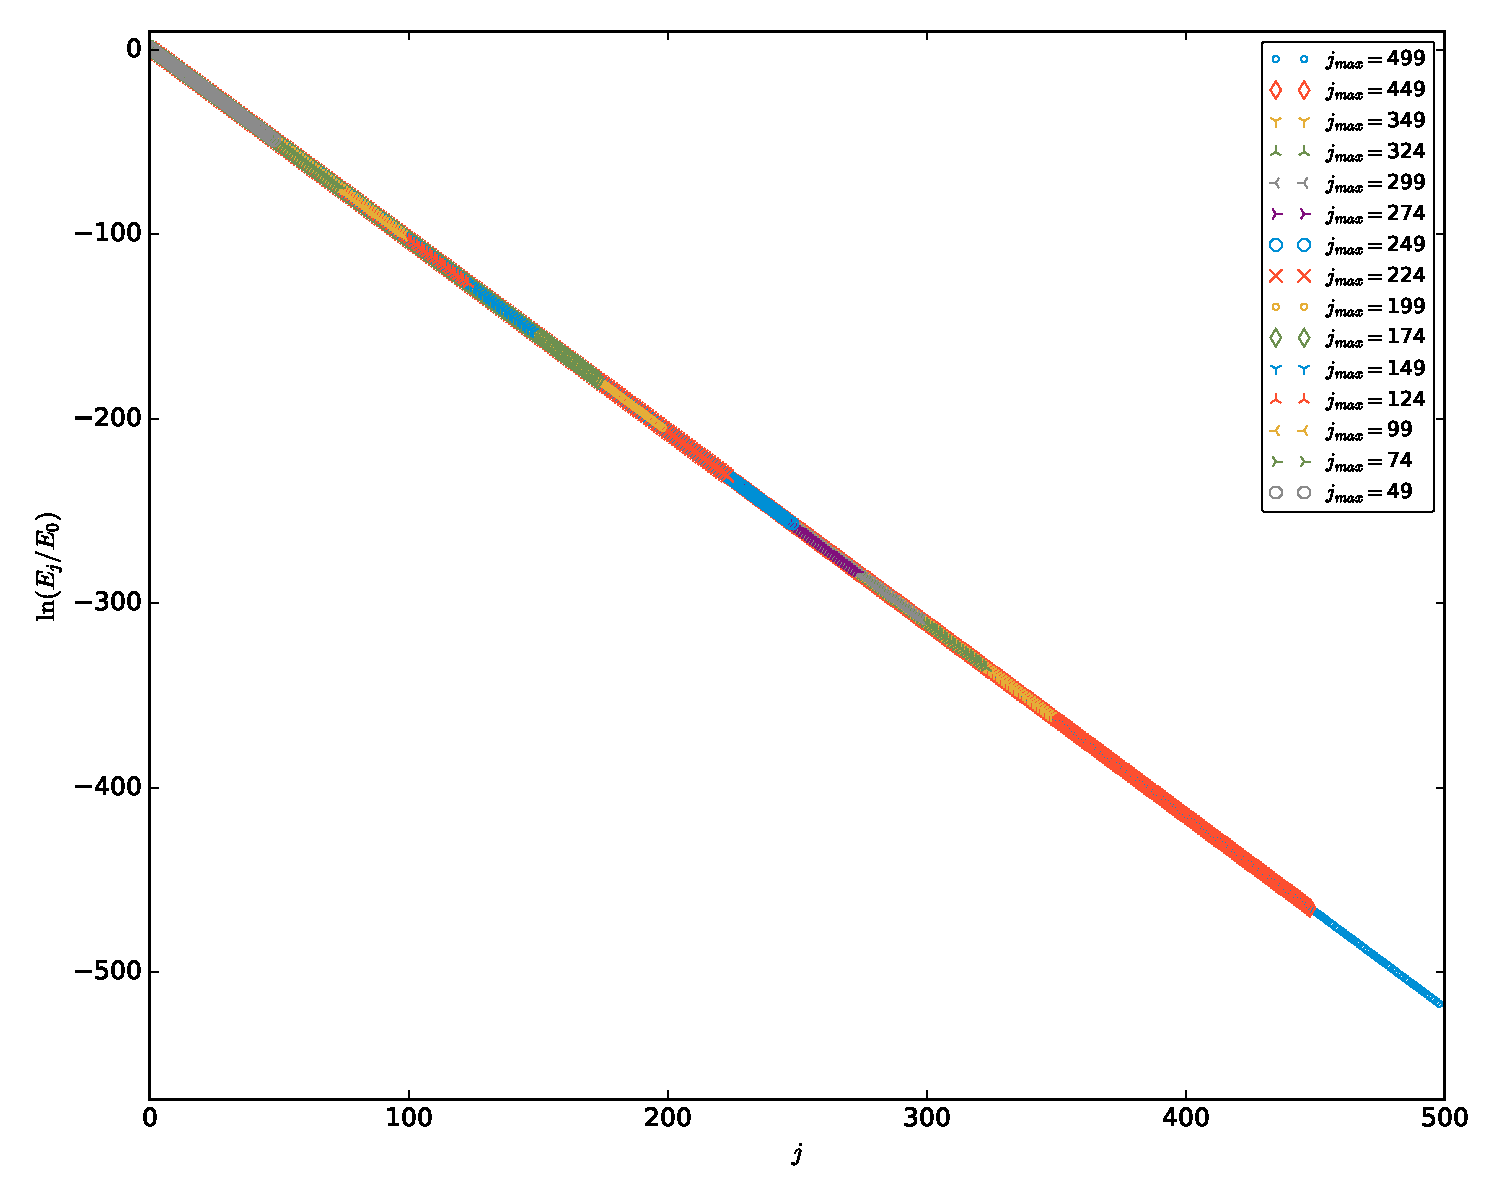
\includegraphics[width=\textwidth]{/Users/bradc/Research/Thesis/PhD/Chapter2/figs/a020_overlay_4paper}
		\caption{An overlay of QP solutions with $\alpha_1 = 0.2$, corresponding to $T_0 \simeq 3.146$.}
		\label{fig: a0.2solns}
	\end{subfigure}
	\:
	\begin{subfigure}[t]{0.45\textwidth}
		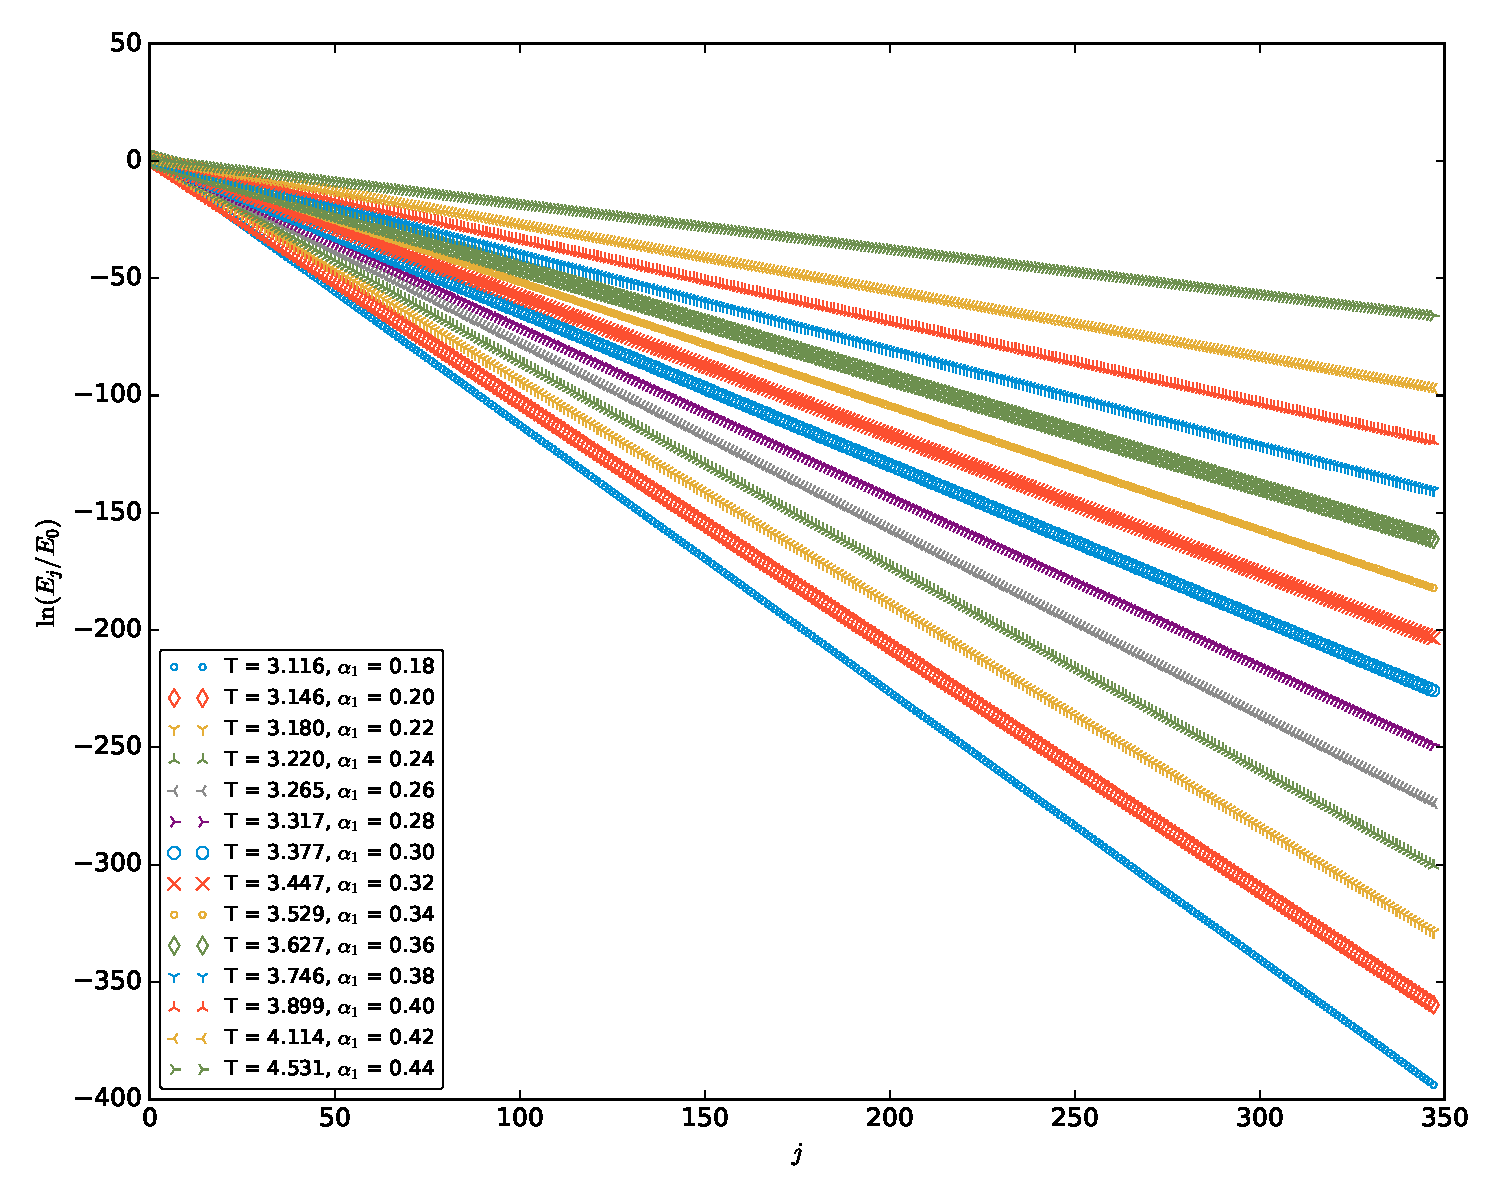
\includegraphics[width=\textwidth]{/Users/bradc/Research/Thesis/PhD/Chapter2/figs/j350_solutions_4paper}
		\caption{Families of QP solutions up to $j_{max}~=~350$.}
		\label{fig: j350 solutions}
	\end{subfigure}
	\caption[Energy spectra for various QP solutions]{Energy spectra for various QP solutions.}
\end{figure}

When examining the range of $\alpha_1$ values that yield QP solutions, it was found that any small $j_{max}$ QP solution could be extended to large $j_{max}$ with proper seeding and sufficient computing power; that is, there seem to be no solutions that exist at low $j_{max}$ that cease to exist at high $j_{max}$\footnote{This is not true for high temperature solutions, as we will see.}. However, a hard limit exists at the maximum $\alpha_1$ value of $\alpha_1=0.442$, corresponding to a temperature of $T \simeq 4.643$. Above this limit, no QP solutions can be found even for $j_{max}$ values as low as $j_{max}=50$. Conversely, there is no lower limit to $\alpha_1$ values; as $\alpha_1 \to 0$ with $\alpha_j > \alpha_{j+1}$, the TTF solution approaches the well-known single-mode solution.

%%%%%%%%%%%%%%%%%%%%%%%%%%%%%%%%%%%%%%%%%
%%%%%%%%%%%%%%%%%%%%%%%%%%%%%%%%%%%%%%%%%

\section{High Temperature Perturbations}
\label{ssec: highT}

In \cite{1507.08261}, additional QP solutions were found by repeatedly perturbing away from existing solutions: the addition of some energy $\delta E$ corresponds to the changes $\alpha_j \to \alpha_j + u_j$ and $\beta_j \to \beta_j + \theta_1 + \omega_j \theta_2$. The perturbed quantities are given by the system of linear equations
\begin{align}
\label{HT1}
\delta E &= 4 \sum_j \omega^2_j \alpha_j u_j \\
\label{HT2}
\delta N &= 4 \sum_j \oj \alpha_j u_j = 0 \\
\label{HT3}
0 &= \ol \left( \alpha_\ell (\theta_1 + \ol \theta_2) +\beta_\ell u_\ell \right) + 6T_\ell \alpha_\ell^2 u_\ell + 2 \sum_{i \neq \ell} R_{i\ell} (\alpha_i^2 u_\ell + 2 \alpha_i \alpha_\ell u_\ell ) \nonumber \\
& + 2 \stackrel{\ell \leq i + j}{\sum_{i \neq \ell} \sum_{j \neq \ell}} S_{ij(i+j-\ell)\ell} \left[ u_i \alpha_j \alpha_{i+j-\ell} + u_j \alpha_i \alpha_{i+j-\ell} + \alpha_i \alpha_j u_{i+j-\ell} \right].
\end{align}
Therefore, by solving \eqref{HT1}-\eqref{HT3} for $\{ u_j, \theta_1, \theta_2 \}$, the existing QP solution can be updated and the process can be repeated. 

For a standard QP solution with $\alpha_1 = 0.2$, the initial temperature is $T_0 = 3.146$. By applying the high temperature perturbation method described above, we are able to increase the temperature of the solution. However, this process must be examined with some scrutiny; applying repeated perturbations to a known solution does not guarantee the final result remains a valid solution. To investigate this further, we have implemented two high temperature solvers, both of which increment the energy of the system using \eqref{HT1}-\eqref{HT3} and are able to project back to the QP solution plane after a specified number of perturbations. However, the projection used by one solver takes an input $\alpha_1$ value when solving the QP equation \eqref{qp eqn}, while the other holds the temperature of the solution fixed during projection. To hold the temperature fixed, we use the definition of $T$ and the freedom to rescale the $\alpha_j$ such that $\alpha_0 = 1$ to solve for $\alpha_1$ via
\begin{align}
\label{a1 eqn}
\alpha_1^2 = \frac{1}{\omega_1 (T - \omega_1)} \left( \omega_0 (\omega_0 - T) + \sum_{j \geq 2} \omega_j (\omega_j - T) \alpha_j^2 \right)
\end{align}
It can easily be seen that $\alpha_1$ will become singular when $T = \omega_1 = 5$ in AdS$_4$. Since we are inputting a value for the temperature $T$ instead of a $\alpha_1$, we are still solving a system of $j_{max} + 1$ equations for $j_{max} + 1$ unknowns.

%%%%%%%%%%%%%%%%%%%%%%%%%%%%%%%%%%%%%%%%%

\subsection{Projections With $\alpha_1$ as the Input}
\label{ssec: a1 projections}

Let us first consider the results of the $\alpha_1$ projection method, shown in figure~\ref{fig: reop comparisons}. We have fixed the perturbation amount $\delta E$ to $1\%$ of the energy of the initial solution. Beginning with an $\alpha_1 = 0.44$ solution with low \jm, we apply repeated energy perturbations and project back to the QP solution plane with a frequency of once per 5 temperature iterations. Figure~\ref{fig: a_1andTa0.2reop5} shows the resulting values of $\alpha_1$ and $T$ during these perturbations. We see that $\alpha_1$ approaches an attractor solution of $\alpha_1 \simeq 0.43$ with $T \simeq 4.3$. The energy perturbations between the projections are insufficient to escape this local minimum so that repeated projections return the same solution. However, when the projection frequency is decreased to once every 20 iterations, the attractor solution is able to be bypassed (variations of the projection frequency and energy perturbations are discussed in appendix~\ref{app: reop freq}). Note that as the iteration number increases, we actually see a \emph{decrease} in $\alpha_1$ value while the temperature continues to increase. At iteration 150 in figure~\ref{fig: a_1andTa.2reop20}, there is a cusp in $\alpha_1$ and a discontinuity in the temperature. After several hundred iterations, $\alpha_1$ becomes negative.

\begin{figure}[h]
	\centering
	\begin{subfigure}[t]{0.45\textwidth}
		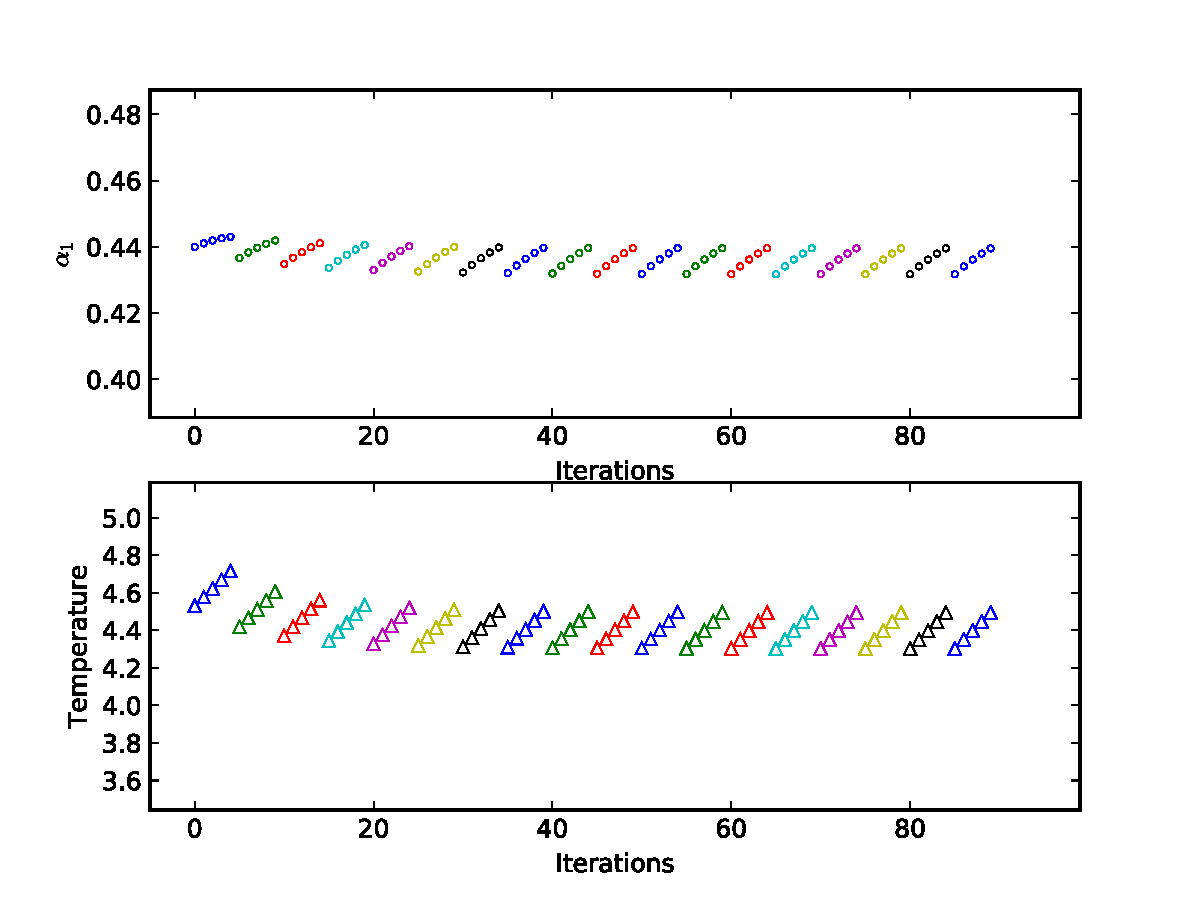
\includegraphics[width=\textwidth]{/Users/bradc/Research/Thesis/PhD/Chapter2/figs/a_1andTvsIteration_reop5}
		\caption{Applying repeated energy perturbations to the initial solution with $\alpha_1=0.44$, projecting back to the QP plane every five iterations.}
		\label{fig: a_1andTa0.2reop5}
	\end{subfigure}
	\:
	\begin{subfigure}[t]{0.45\textwidth}
		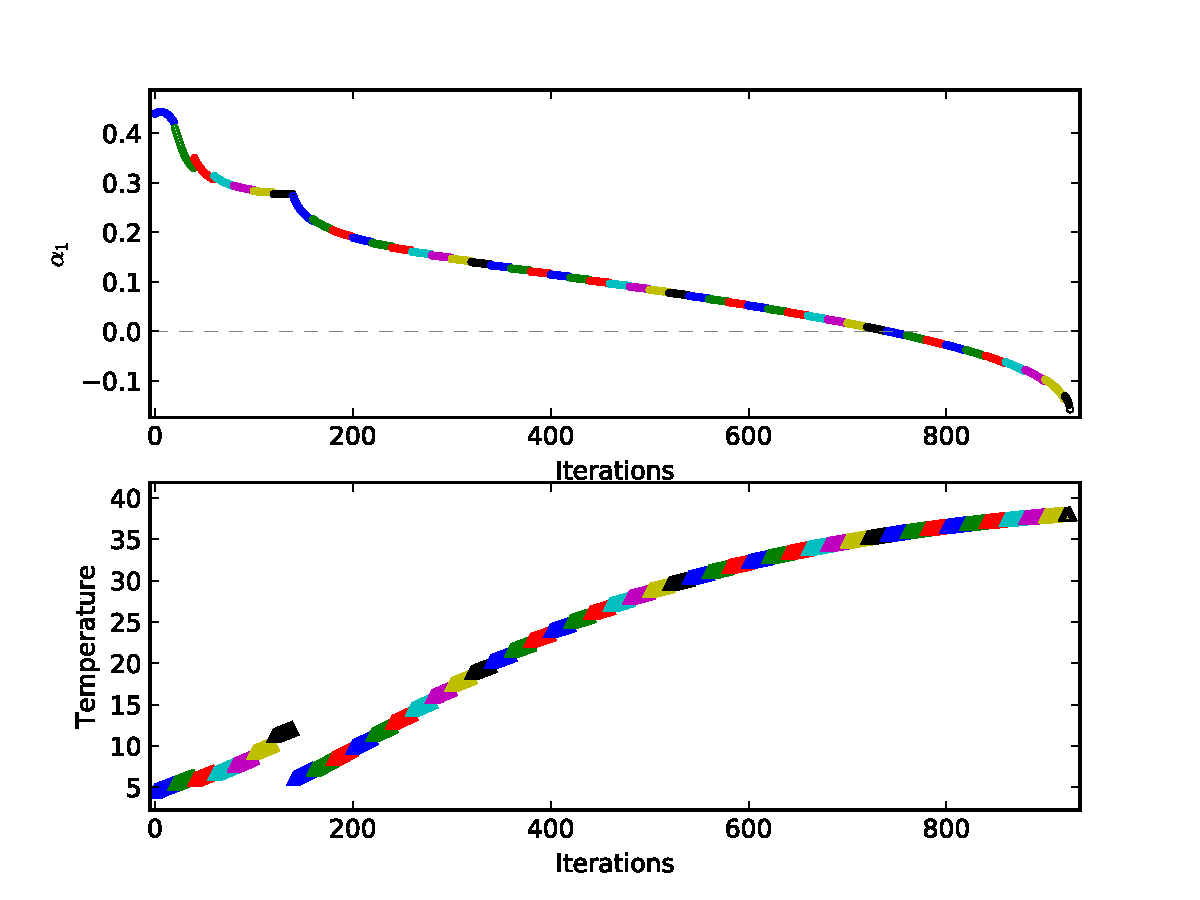
\includegraphics[width=\textwidth]{/Users/bradc/Research/Thesis/PhD/Chapter2/figs/a_1andTvsIteration_reop20}
		\caption{The same QP solution, but projecting back to the QP plane every 20 iterations.}
		\label{fig: a_1andTa.2reop20}
	\end{subfigure}
	\caption[High temperature solutions resulting from projecting back to the QP solution plane at various frequencies]{The results of projecting a $j_{max}=50$, $\alpha_1 = 0.44$ solution back to the QP plane at various frequencies during high temperature perturbations. Colour changes indicate that the solution has been projected back to the QP plane.}
	\label{fig: reop comparisons}
\end{figure}

Let us examine the energy spectra these solutions. In figure~\ref{fig: spec comparisons reop5} we see that when we choose a high projection frequency, the resulting energy spectra do not deviate far from the initial solution (using the $\alpha_1$ projection method) in either shape or temperature. We denote solutions found by this method as ``threshold temperature'' solutions. The values of the threshold temperature $T_{th}$ is robust against increases in $\jm$ and is independent of the starting value of $\alpha_1$, as shown in table~\ref{tab: T_thresh}.

\begin{table}[h]
	\centering
	\begin{tabular}[t]{|c|c|c|}
		\hline
		$\jm$ & $T_{th}$ & Iterations \\ \hline
		$50$ & 4.30344575697724e+00 & $350$ \\ \hline
		$75$ & 4.30344544264076e+00 & $210$ \\ \hline
		$100$ & 4.30344544023857e+00 & $540$ \\ \hline
		$150$ & 4.30344544024198e+00 & $280$ \\ \hline
		$200$ & 4.30344544023915e+00 & $300$ \\ \hline
	\end{tabular}
	\caption[Threshold temperatures for different truncation values with constant projection frequency]{Values of the threshold temperature $T_{th}$ for QP solutions with given $\jm$. Also included is the number of iterations applied (projecting back to the solution plane after every five iterations).}
	\label{tab: T_thresh}
\end{table}

When the projection frequency is decreased, the temperature is able to exceed $T_{th}$. However, as seen in figure~\ref{fig: spec comparisons reop20}, projections back to the QP plane give $\alpha_1 < 0$ and an energy spectrum that is no longer $C^1$ differentiable ({\it c.f.} spectra of iterations 120 and 180). This in itself is not necessarily a breakdown of the quasi-periodic nature of the solution, as $\alpha_j < 0$ if {$\beta_j \tau = (2n + 1) \pi$} for {$n \in \mathbb{N}^0$}. However, upon examining the condition number of the matrix formed by \eqref{HT1}-\eqref{HT3}, we find that in fact the problem becomes ill-conditioned. This results in a absolute value of $u_i$ that is greater than $\alpha_i$; that is, the perturbative condition required to derive the system of linear equations \eqref{HT1}-\eqref{HT3} breaks down. For many prospective high-temperature solutions, this break-down of the perturbative condition is signalled by the loss of $C^1$ differentiability in the energy spectrum due to the values of $\alpha_j$ becoming negative. 

\begin{figure}[h]
	\centering
	\begin{subfigure}[t]{0.45\textwidth}
		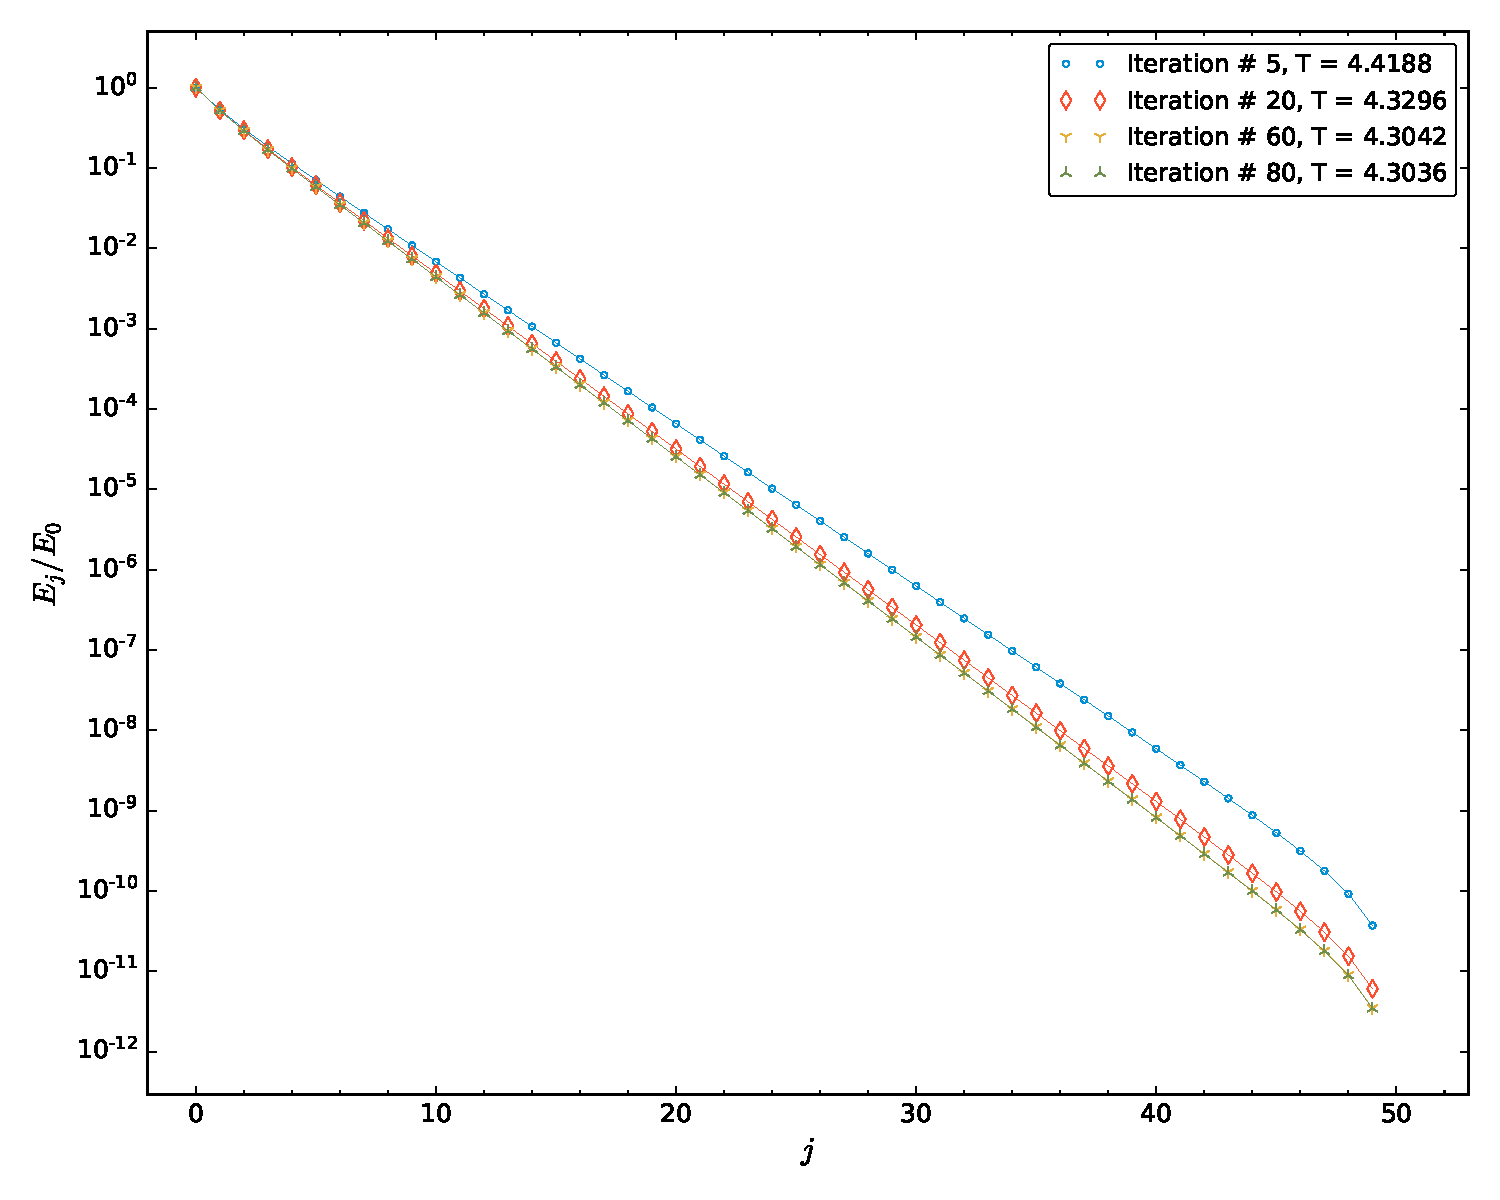
\includegraphics[width=\textwidth]{/Users/bradc/Research/Thesis/PhD/Chapter2/figs/spectracomp_a044_reop5_4paper}
		\caption{Energy spectra when projecting back to the QP solution plane every 5 iterations for an initial $\alpha_1 = 0.44$, QP solution (see figure~\ref{fig: a_1andTa0.2reop5} for temperature and $\alpha_1$ as a function of iteration).}
		\label{fig: spec comparisons reop5}
	\end{subfigure}
	\:
	\begin{subfigure}[t]{0.45\textwidth}
		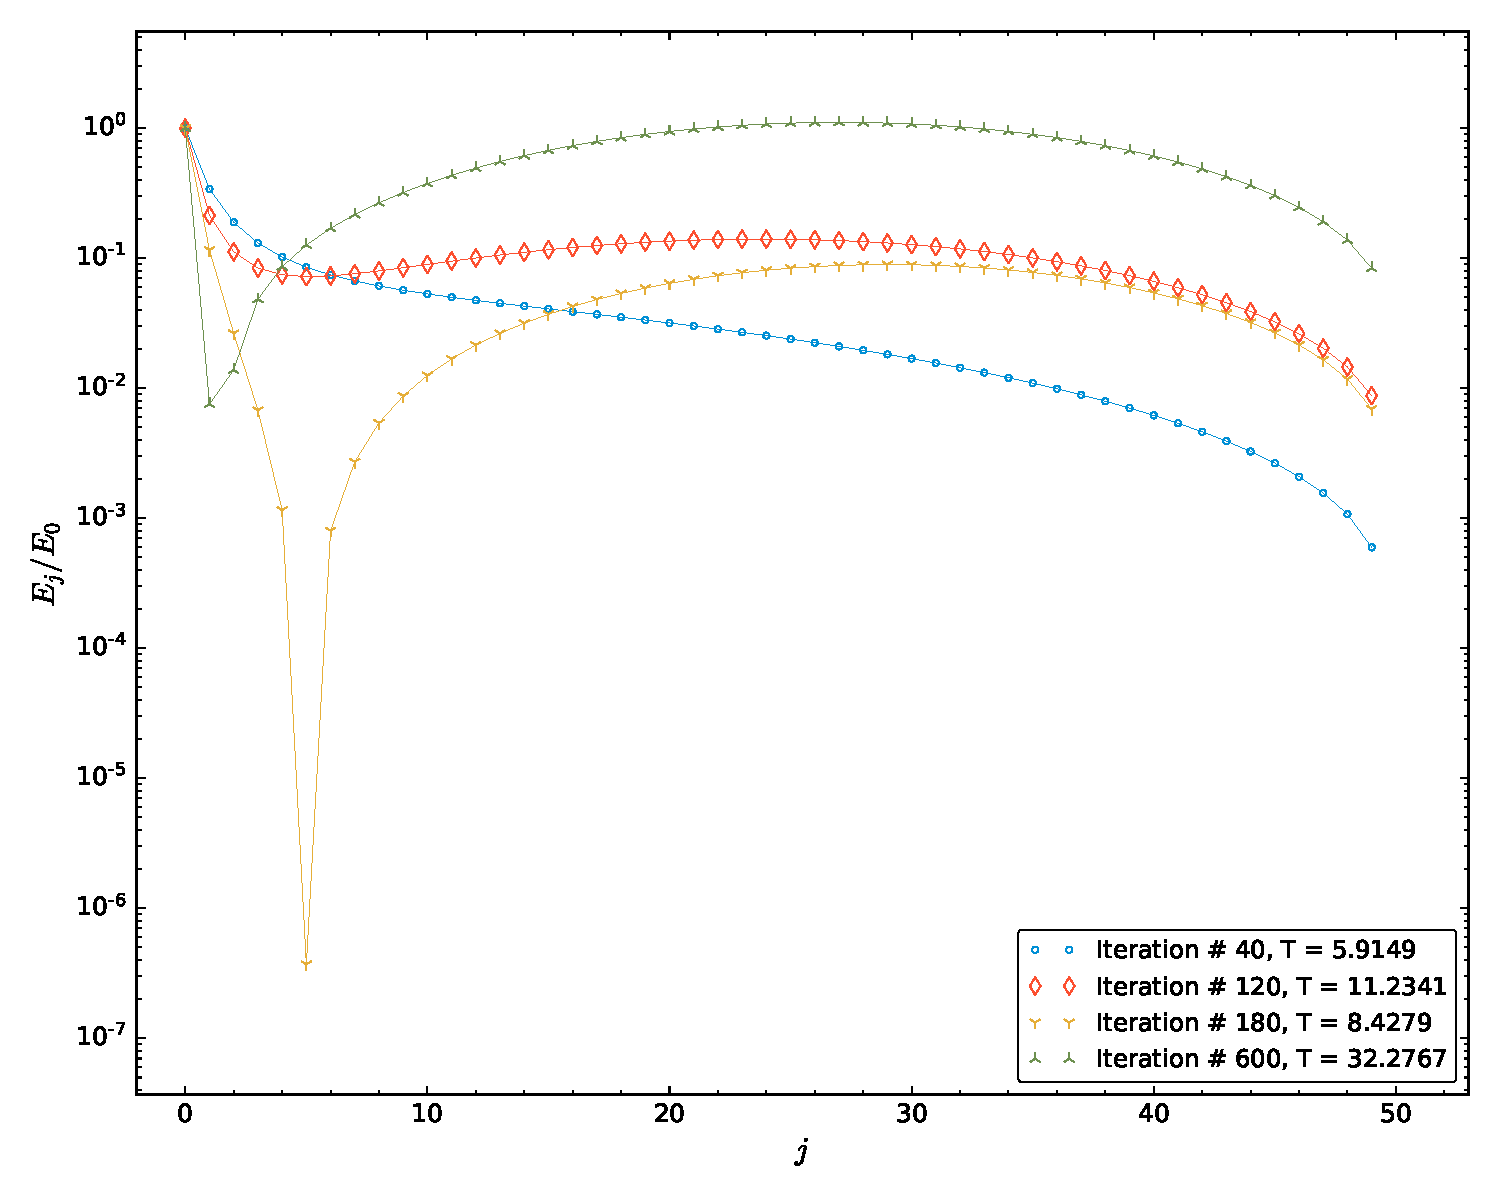
\includegraphics[width=\textwidth]{/Users/bradc/Research/Thesis/PhD/Chapter2/figs/spectracomp_a044_reop20_4paper}
		\caption{The same initial QP solution as figure~\ref{fig: spec comparisons reop5} is used, but is projected back to the QP plane every 20 iterations.}
		\label{fig: spec comparisons reop20}
	\end{subfigure}
	\caption[Energy spectra resulting from perturbing the same QP solution at differing frequencies]{Comparing energy spectra of high-temperature perturbations of an $\alpha_1=0.44$ QP solution that have been projected back to the QP plane at different frequencies.}
	\label{fig: spec comps with reop}
\end{figure}


%%%%%%%%%%%%%%%%%%%%%%%%%%%%%%%%%%%%%%%%%

\subsection{Projections at Constant Temperature}
\label{ssec: T projections}

We again use a series of small energy perturbations to seek high-temperature QP solutions, this time using a constant-temperature projection method at regular intervals. Starting from a standard $\alpha_1 = 0.44$ QP solution, perturbations are applied to increase the temperature. After five increments, the temperature is calculated and used as the input to the second nonlinear solver. This ensures that the temperature is not changed when projecting back to the solution plane. Goal temperatures of $T=5.5$, $6.0$, and $7.0$ were chosen -- when the solution reached or exceeded this temperature, it would be projected back to the QP plane and the perturbations would cease. The resulting spectra for each temperature goal over several choices of $\jm$ are shown in figure~\ref{fig: const T perturbs}. It is worth noting that $\jm = 250$ spectra are not included for temperature goals of $T=6.0$ and $7.0$ because the constant-temperature projection failed to find a solution.

\begin{figure}[h]
	\centering
		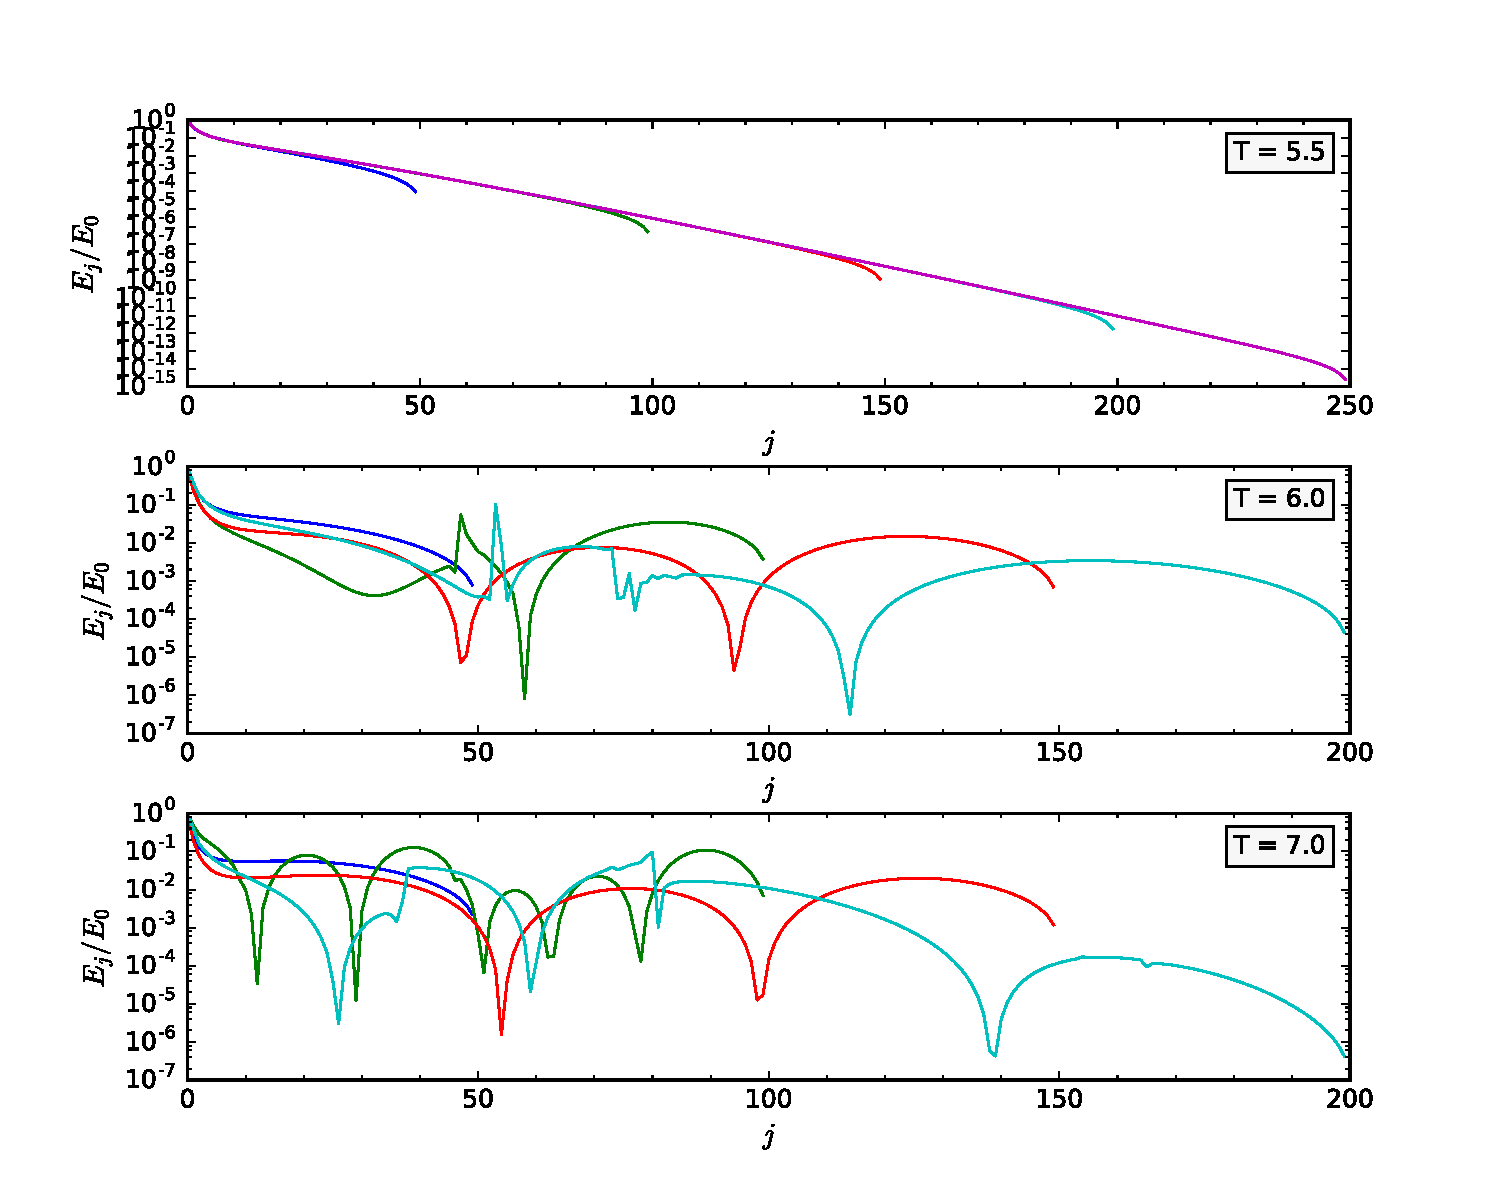
\includegraphics[width=\textwidth]{/Users/bradc/Research/Thesis/PhD/Chapter2/figs/HighTemperatureComparison}
		\caption{Finding high temperature QP solutions using repeated perturbations with regular projections back to the QP plane.}
		\label{fig: const T perturbs}
\end{figure}

Recall that solutions must be robust in the limit of $\jm \to \infty$ in order to be considered solutions to the full TTF theory. While the upper panel of figure~\ref{fig: const T perturbs} suggests that solutions with temperatures at or near $T=5.5$ can be constructed in the large-$\jm$ limit, it is clear that goal temperatures of $T=6.0, 7.0$ do not support solutions to the full TTF theory. In fact, when solutions were not projected back to the QP plane at regular intervals during the energy perturbations, no solutions at all could be found when the temperature was held fixed. It would seem that the domain of high temperature QP solutions is restricted to a narrow region near the QP plane defined by \eqref{qp eqn}. 

%%%%%%%%%%%%%%%%%%%%%%%%%%%%%%%%%%%%%%%%%

\subsection{Building High-Temperature Solutions}
\label{ssec: by hand highT}

In figure~\ref{fig: const T perturbs} we see that continuous spectra exist for goal temperatures of $T=6.0$ and $7.0$ when $\jm = 50$. It is therefore reasonable to consider whether a high temperature, low $\jm$ solution could be extended to a high temperature, high $\jm$ solution using a fitting procedure similar to that used in \S~\!\ref{ssec: large jmax} to find quasi-periodic solutions. Instead of fitting $\alpha_j$ values away from the highest modes, we instead apply the tail fitting the final 5 modes and use the fit to generate seed values for a $\jm + 5$ solution. We see in figure~\ref{fig: manual highT} that this method results in spectra where energy becomes increasingly concentrated in high-$j$ modes. In fact, for solutions with $\jm \geq 90$, and equal or greater amount of energy resides in the high-$j$ modes than in the zero-mode. These solutions are not robust as $\jm \to \infty$ and therefore are not solutions to the TTF equations.

\begin{figure}[h]
	\centering
	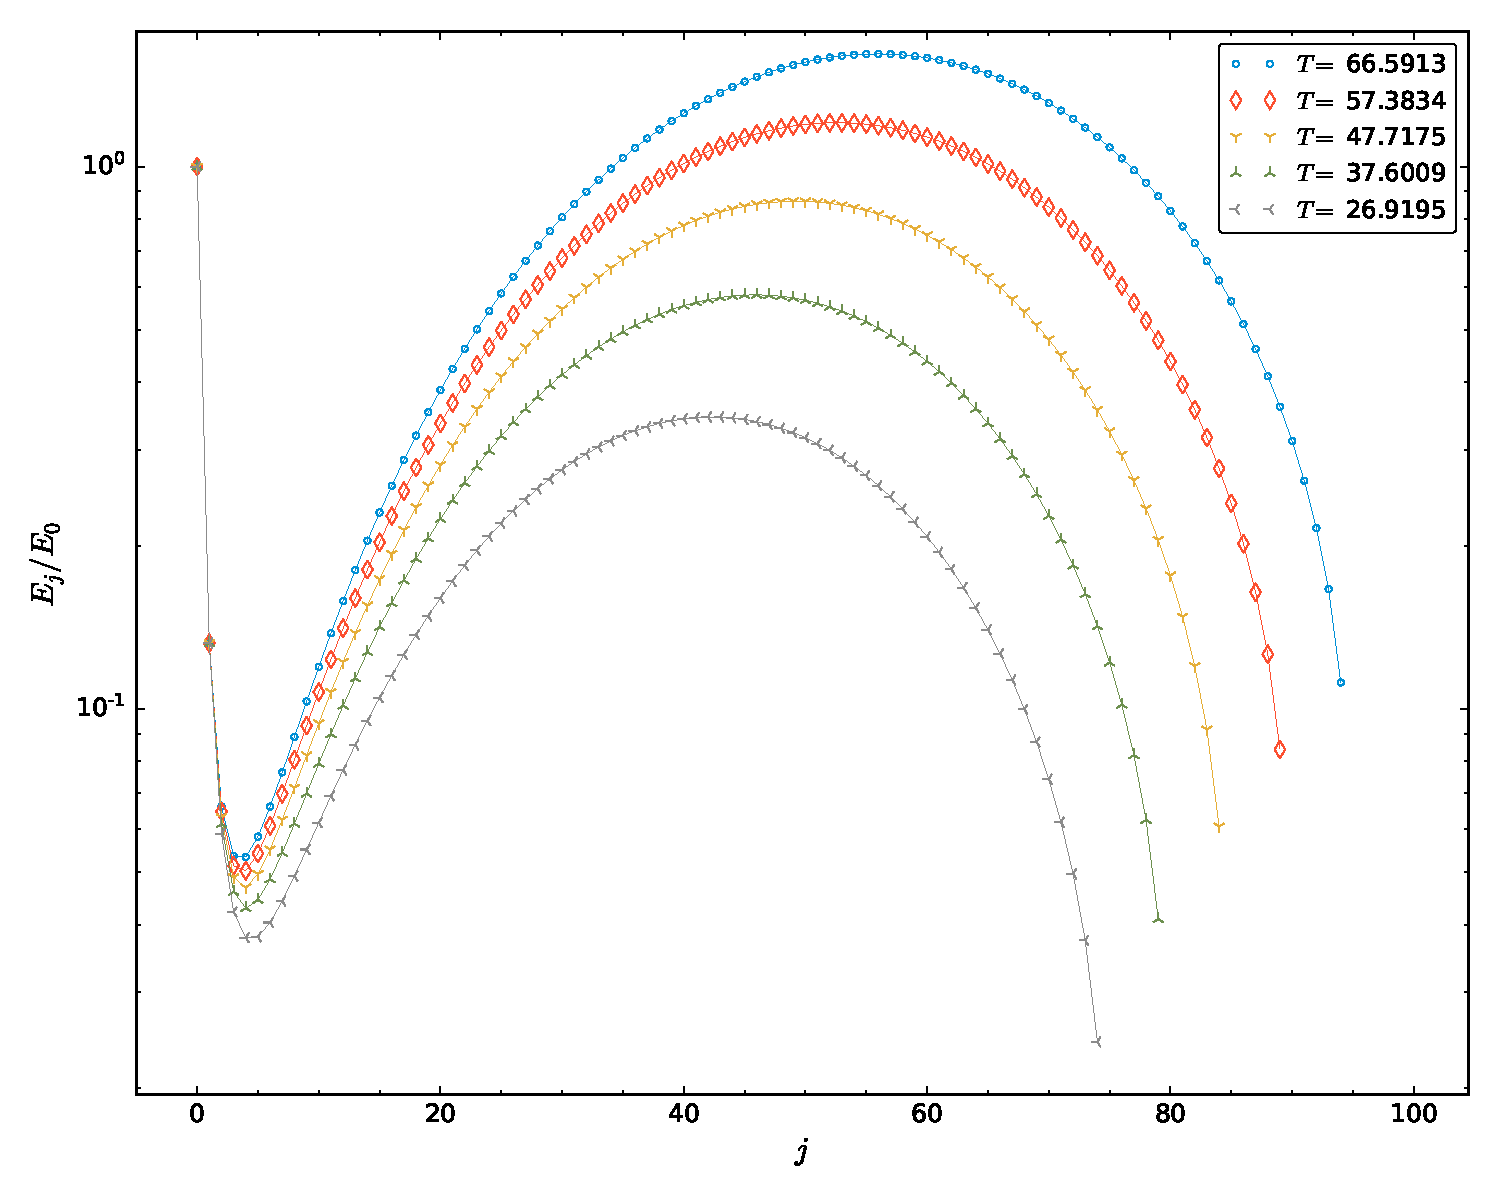
\includegraphics[width=0.75\textwidth]{/Users/bradc/Research/Thesis/PhD/Chapter2/figs/T30_extend_highj_4paper}
	\caption[Constructing high temperature solutions by hand]{Extending a high temperature, low $\jm$ solution to higher temperatures by fitting the final 5 modes and generating seed values.}
	\label{fig: manual highT}
\end{figure}


%Despite high-temperature solutions being inaccessible via repeated energy perturbations, we may ask if such solutions can be found by using different methods. First, we consider perturbing a known QP solution to a high temperature \emph{without} regular projections back to the QP plane. Then, at some sufficiently high temperature $T_{max}$, we attempt to project back to the QP plane. In figure~\ref{fig: T30 vs j_max}, the spectra of QP solutions before and after projection are shown for increasing $j_{max}$. For solutions with $\jm \geq 100$, high-temperature solutions are in fact projected to low-temperature solutions that may contain negative $\alpha_j$ values. Low-$\jm$ solutions, however, appear to remain at high-temperatures after projecting back to the plane. We use this type of solution in our next method.
%\begin{figure}[h]
%	\centering
%	\begin{subfigure}[t]{0.45\textwidth}
%		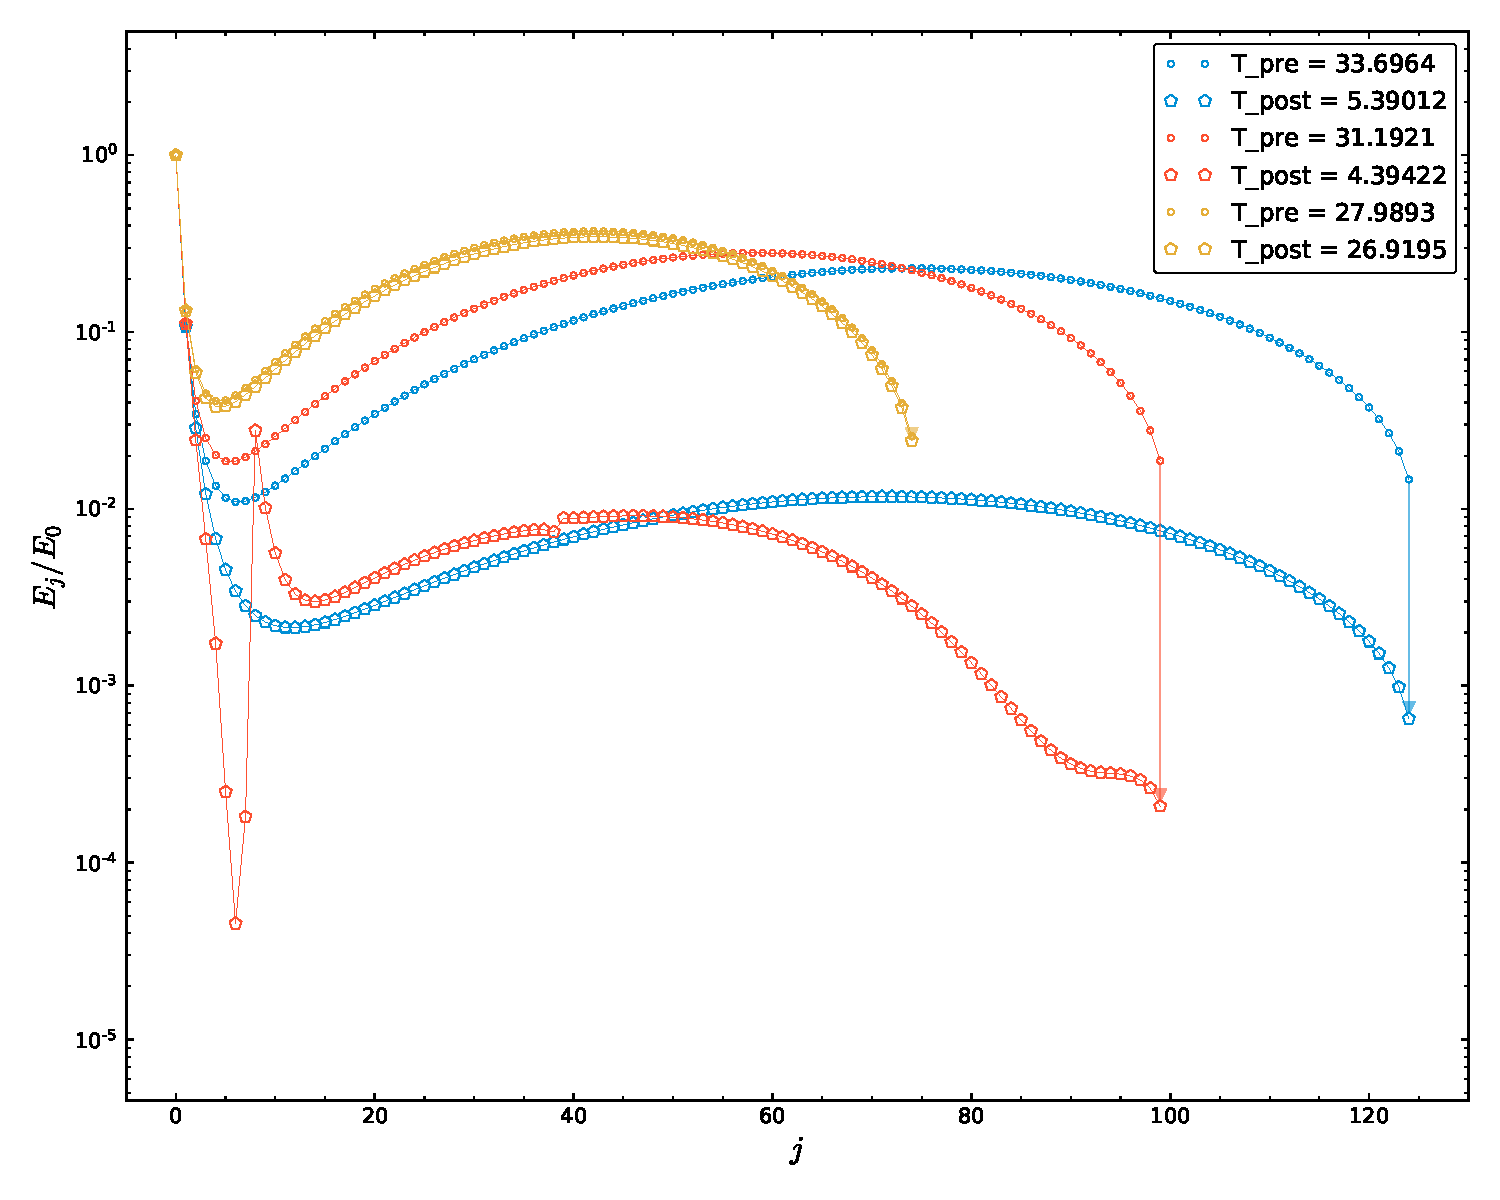
\includegraphics[width=\textwidth]{/Users/bradc/Research/Thesis/PhD/Chapter2/figs/T30vsj_max_partial_4paper}
%		\caption{QP solutions perturbed to $T_{max}=30.00$, which were then used as seeds for the nonlinear solver. Arrows are oriented from pre-optimized to post-optimized solutions.}
%		\label{fig: T30 vs j_max}
%	\end{subfigure}
%	\;
%	\begin{subfigure}[t]{0.45\textwidth}
%		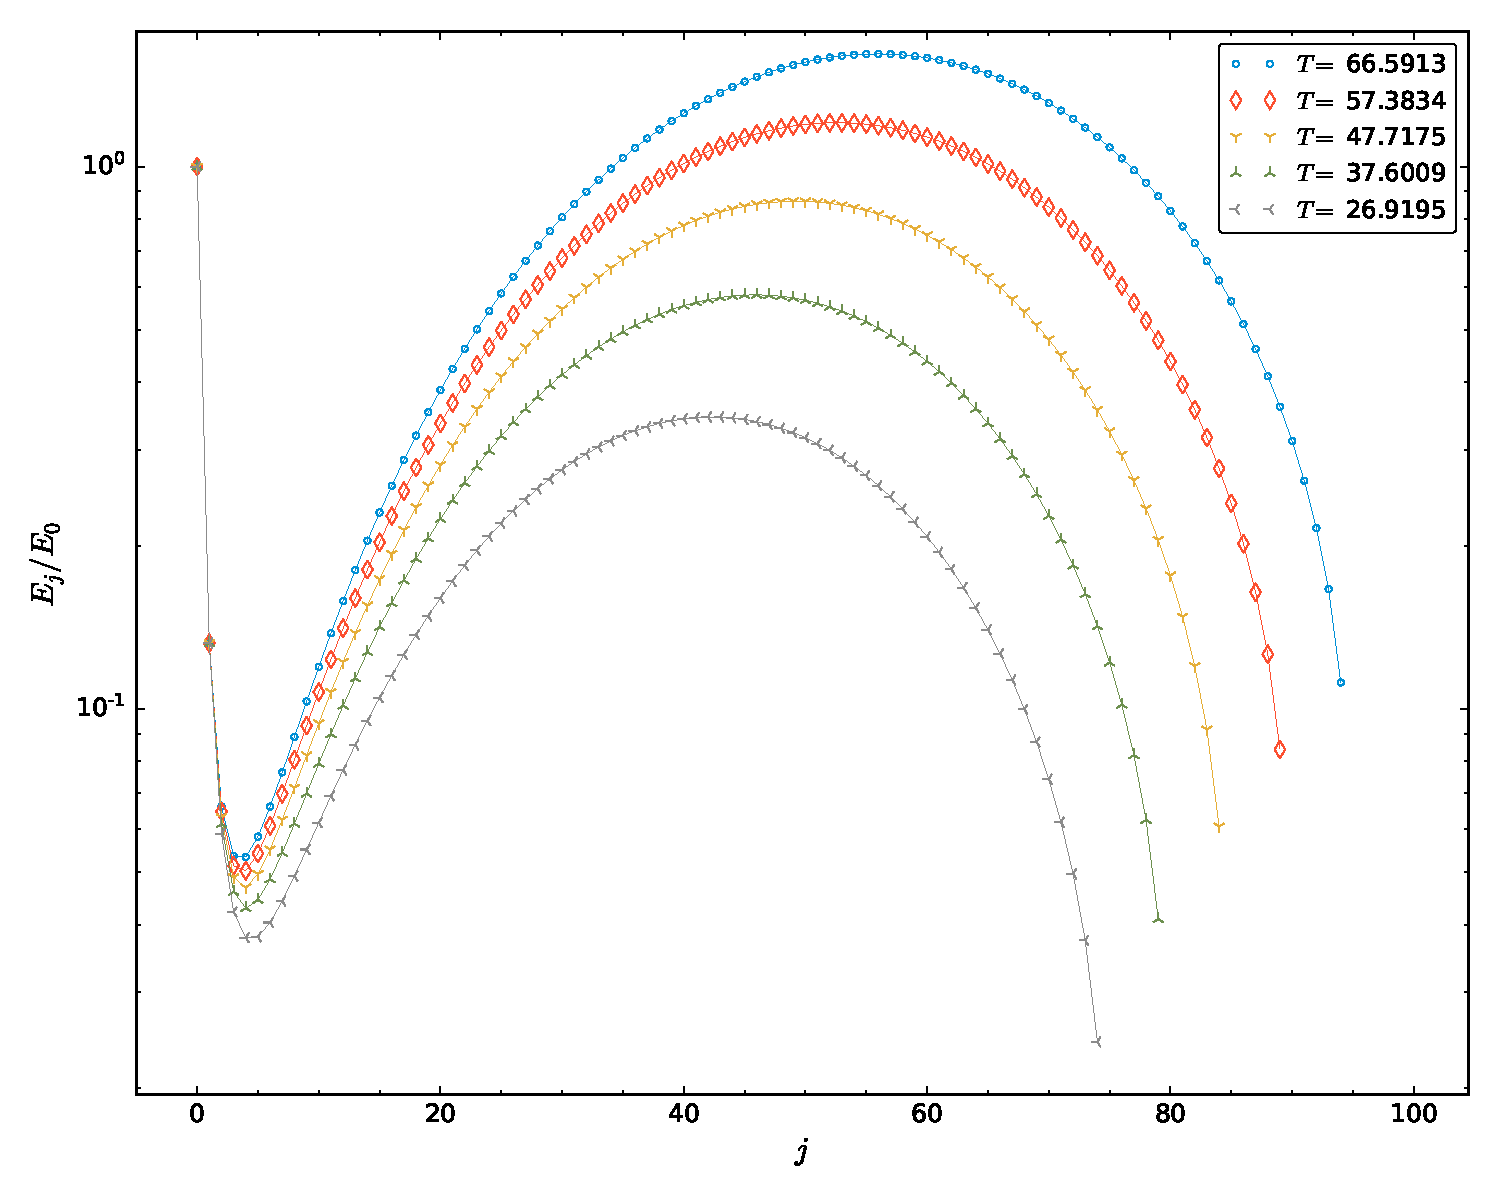
\includegraphics[width=\textwidth]{/Users/bradc/Research/Thesis/PhD/Chapter2/figs/T30_extend_highj_4paper}
%		\caption{Extensions of the $j_{max}=50$ solution from figure~\ref{fig: T30 vs j_max} to larger $j_{max}$ solutions using tail fitting on only the final 5 modes of the solution.}
%		\label{fig: manual highT}
%	\end{subfigure}
%	\caption[Constructing high temperature solutions by hand]{Constructing high temperature solutions ``by hand.''}
%	\label{fig: making highT}
%\end{figure}


%%%%%%%%%%%%%%%%%%%%%%%%%%%%%%%%%%%%%%%%%

\subsection{Stability of QP Solutions}

Having identified QP solutions that are robust in the limit of $\jm \to \infty$, as well as a class of higher temperature solutions found from incremental perturbations about QP solutions, we can now ask how these solutions would evolve within the perturbative description. In particular, we wish to examine possible direct and inverse energy cascades in these quasi-periodic solutions, and determine if they continue to represent stable data. The cascades of energy between length scales will be evident in the spectra. Indirect observations of stability can be made through the value of the Ricci scalar at the origin, since large absolute values and/or rapid increases in scalar curvature often indicate instability in numerical simulations {\bf (ref?)}. 

Another indicator of possible collapse and/or violation of the perturbative approximation is the growth of residuals when the TTF solutions are substituted into the Einstein equations. The residuals are calculated by reconstructing the time dependence of the scalar field and its derivatives using the amplitude-phase variables, and comparing the $\mc O(\epsilon^2)$ values of the derivatives of the metric functions in \eqref{EE const1}-\eqref{EE const2}. In particular, using the numerical values of the amplitude-phase variables $A_j$ and $B_j$, \eqref{ttf phi} gives the value of the leading-order scalar field contribution, $\phi_1(t,x)$. The $\mc O(\epsilon^2)$ contribution to the derivatives of metric functions come from
\begin{align}
\label{ddelta}
\p_x \delta_2(t,x) &= -\sin(x) \cos(x) \left( (\p_x \phi_1)^2 + (\p_t \phi_1)^2 \right) \, , \\
\label{dA}
\p_x A_2(t,x) &= -\frac{1 - d + \cos(2x)}{\sin(x) \cos(x)}(A_2 - 1) - \sin(x) \cos(x) \left( (\p_x \phi_1)^2 + (\p_t \phi_1)^2 \right) \, , \\
\text{with} \; A_2(t,x) &= - \frac{\cos^d(x)}{\sin^{d-1}(x)} \int^x_0 \tan^{d-1}(y) \left( (\p_t \phi_1)^2 + (\p_x \phi_1)^2 \right) dy \, .
\end{align}
The $L^2$-norm of the differences between \eqref{ddelta}-\eqref{dA} and \eqref{EE const1}-\eqref{EE const2} would constitute the residuals of the Einstein equations. However, while the leading-order contribution to the residuals is $\mc O(\epsilon^4)$, there are in fact higher order terms that enter into the calculation of $\p_t \phi$. A careful evaluation of the constraints would therefore include calculating the $\mc O(\epsilon^4)$ term in the metric function $A(t,x)$ so that the product $A ( \Phi^2 + \Pi^2)$ would include terms $\mc O(\epsilon^6)$. Instead, we limit our focus to examining only the difference between \eqref{EE const1} and \eqref{ddelta}, which does not suffer from higher-order contributions. The examination of residuals is taken as a suggestion of how well a TTF solution continues to satisfy the Einstein equations throughout its evolution, with the understanding that growing residuals would indicate that higher order terms in the perturbative expansion are becoming relevant.

%%%%%%%%%%%%%%%%%%%%%%%%%%%%%%%%%%%%%%%%%
%%%%%%%%%%%%%%%%%%%%%%%%%%%%%%%%%%%%%%%%%

\section{Time Evolution of Quasi-Periodic Solutions}
\label{sec: time evolution}

The weakly turbulent behaviour of the scalar field in the TTF is captured by the $\mc O(\epsilon^2)$ renormalization group flow equations {\eqref{RN1}-\eqref{RN2}}. Having identified different families of quasi-periodic solutions, we wish to evolve these solutions and examine the direct and inverse cascades responsible for balancing the flow of energy between long and short length scales. To do this, we use numerical methods first described by \cite{1606.02712}, and take solutions discussed in \S\!~\ref{sec: qp} as initial data.

{\bf $\jm = 100$, $\alpha_1 = 0.2$, $T=3.146$}

The fraction of the total energy in each mode during the evolution of a $\jm = 100$, $T = 3.146$ QP solution with $\epsilon = 0.01$ is shown in figure~\ref{fig:qpevo}. We see that energy in the lowest-$j$ modes remains constant over the duration of the evolution, while the fraction in the highest-$j$ modes increases after $\tau \simeq 0.3$. Similar behaviour is observed for higher $\jm$ solutions and over values of $0.2 \leq \alpha_1 \leq 0.44$. Given the scale of the energy in the modes $j \geq 96$, the growing energy fractions in these modes can mainly be attributed to numerical errors rather than turbulent cascades.

\begin{figure}[h]
	\centering
	\begin{subfigure}[t]{0.45\textwidth}
		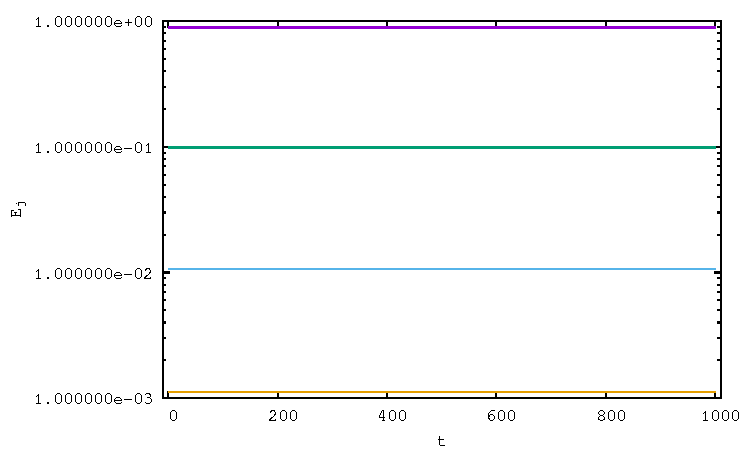
\includegraphics[width=\textwidth]{/Users/bradc/Research/Thesis/PhD/Chapter2/figs/QPa2_00e-01_j100_lowjenergyevo}
		\caption{From top to bottom: $j=0, 1, 2, 3$ (purple, green, blue, orange).}
	\end{subfigure}
	\;
	\begin{subfigure}[t]{0.45\textwidth}
		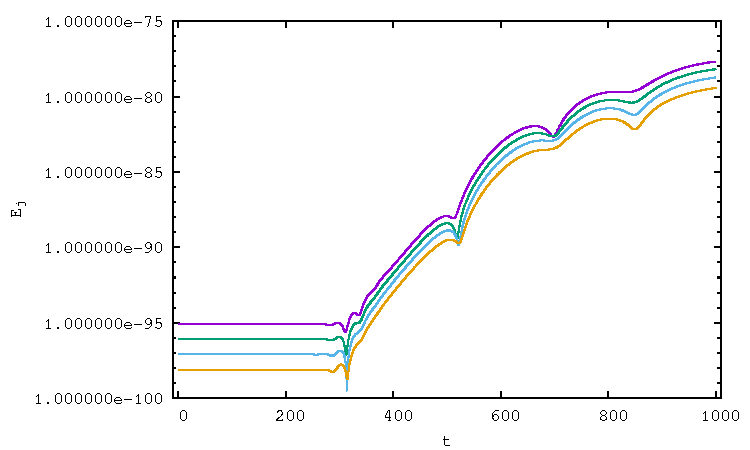
\includegraphics[width=\textwidth]{/Users/bradc/Research/Thesis/PhD/Chapter2/figs/QPa2_00e-01_j100_highjenergyevo}
		\caption{From top to bottom: $j=96, 97, 98, 99$ (purple, green, blue, orange).}
	\end{subfigure}
	\caption[Evolution of QP solutions at low temperature]{Fraction of the total energy in each mode during evolution of an $\alpha_1 = 0.2$, $\jm = 100$, QP solution with $\epsilon=0.01$.}
	\label{fig:qpevo}
\end{figure}

%To better understand how well such solutions continue to satisfy the TTF equation throughout their time evolution, we evaluate the residuals of \eqref{qp eqn} at regular intervals of $t=0.025$ during the evolution of a $\jm = 100$, $T=4.531$ QP solution using data taken during the evolution. Figure~\ref{fig: Qpa4_40e-01QPresids} is a sample of the $L^2$-norm of these residuals for 

%\begin{figure}[h]
%	\centering
%	\begin{subfigure}[t]{0.45\textwidth}
%		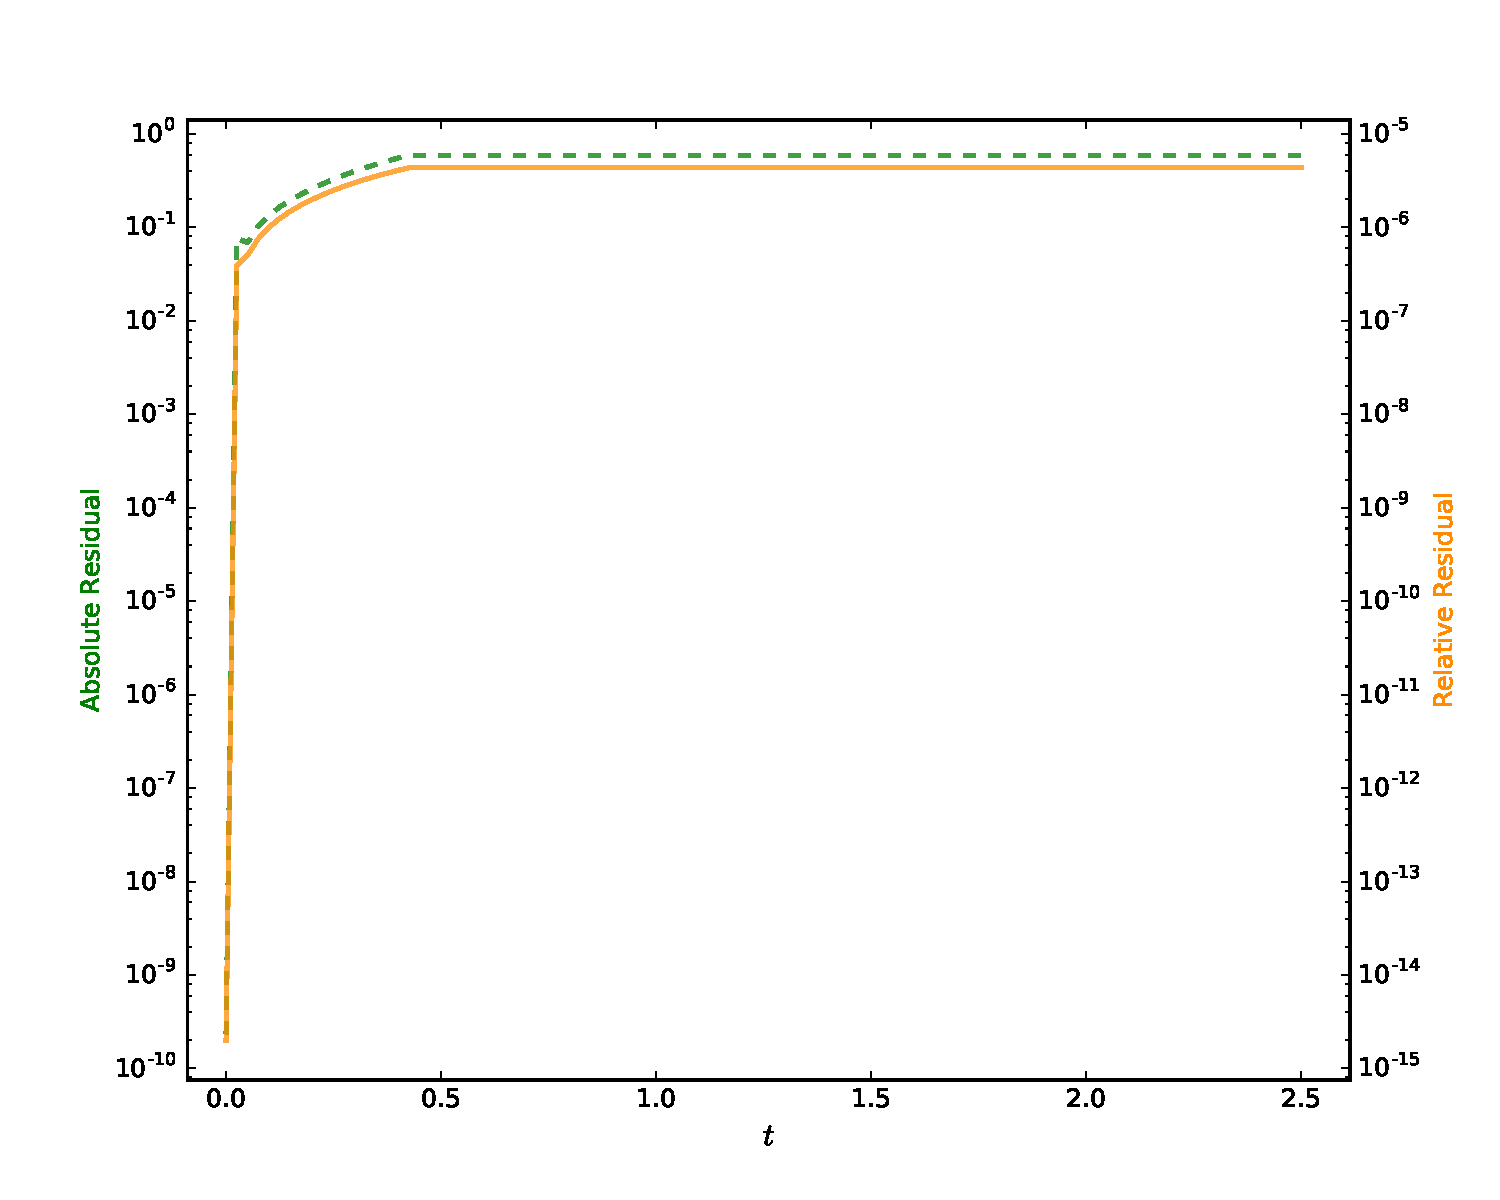
\includegraphics[width=\textwidth]{/Users/bradc/Research/Thesis/PhD/Chapter2/figs/Qpa4_40e-01QPresids}
%	\end{subfigure}
%	\;
%	\begin{subfigure}[t]{0.45\textwidth}
%		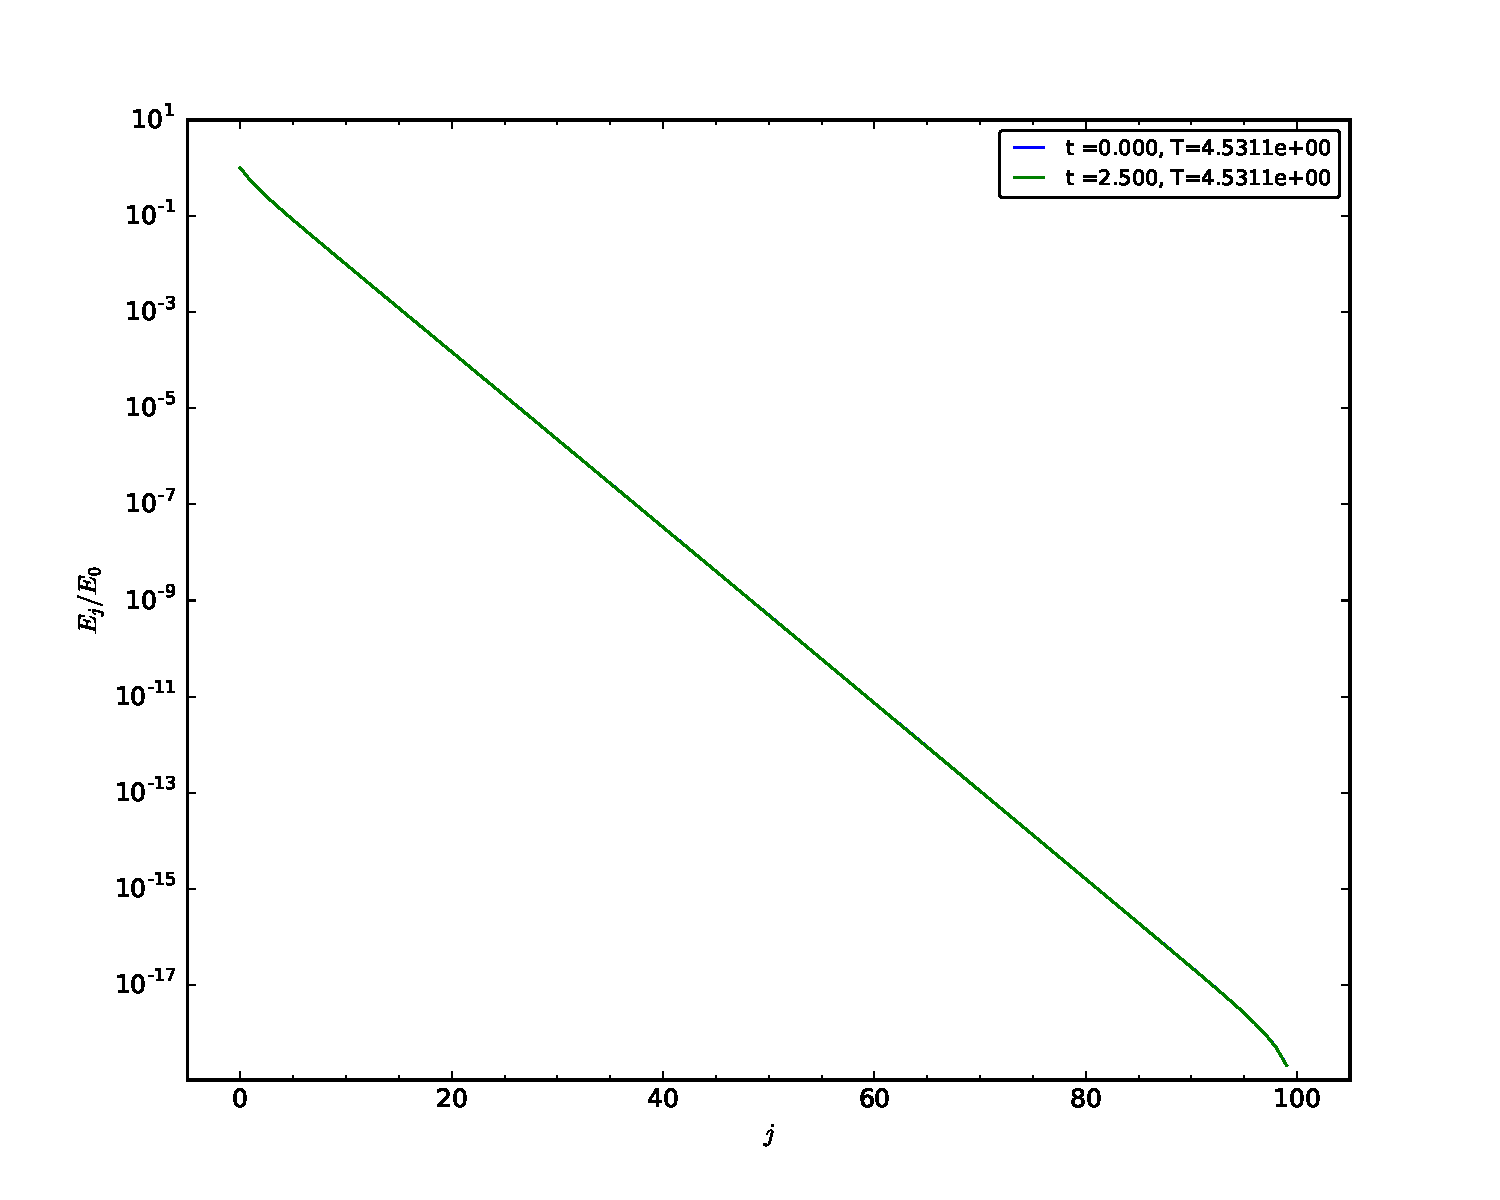
\includegraphics[width=\textwidth]{/Users/bradc/Research/Thesis/PhD/Chapter2/figs/Qpa4_40e-01specevo}
%	\end{subfigure}
%	\caption[Residual and spectrum of a low-temperature QP solution during evolution]{{\it Left:} $L^2$-norm of the residuals of \eqref{qp eqn} evaluated at intervals of $0.025$ during the evolution of a $\jm = 100$, $\alpha_1 = 0.44$ QP solution with $\epsilon = 0.1$. {\it Right:} The spectra of the QP solution at the beginning and end of the evolution.}
%	\label{fig: Qpa4_40e-01QPresids}
%\end{figure}

Furthermore, we can attempt to project the evolved solutions back to the QP plane at various times to explore if these solutions lose their quasi-periodic nature. We observe that the time-evolved, low-temperature QP solutions are easily projected back to the solution plane at all times during the evolution, and that the resulting solutions solve the QP equation \eqref{qp eqn} to a high degree of accuracy (see figure~\ref{fig: Qpa4_40e-01j100EvolutionProjection}). While this is to be expected for such low-temperature QP solutions, we will soon see that even padding a known QP solution with zeros causes the loss of quasi-periodicity during evolution. For comparison, figure~\ref{fig: QPa4_40e-01padj200_evolutionprojection} shows the results of attempting to project a QP solution that has been padded with zeros back to the QP plane during its evolution. Note the scale on the plot of the $L^2$-norm in either case.

\begin{figure}[h]
	\centering
	\begin{subfigure}[t]{0.45\textwidth}
		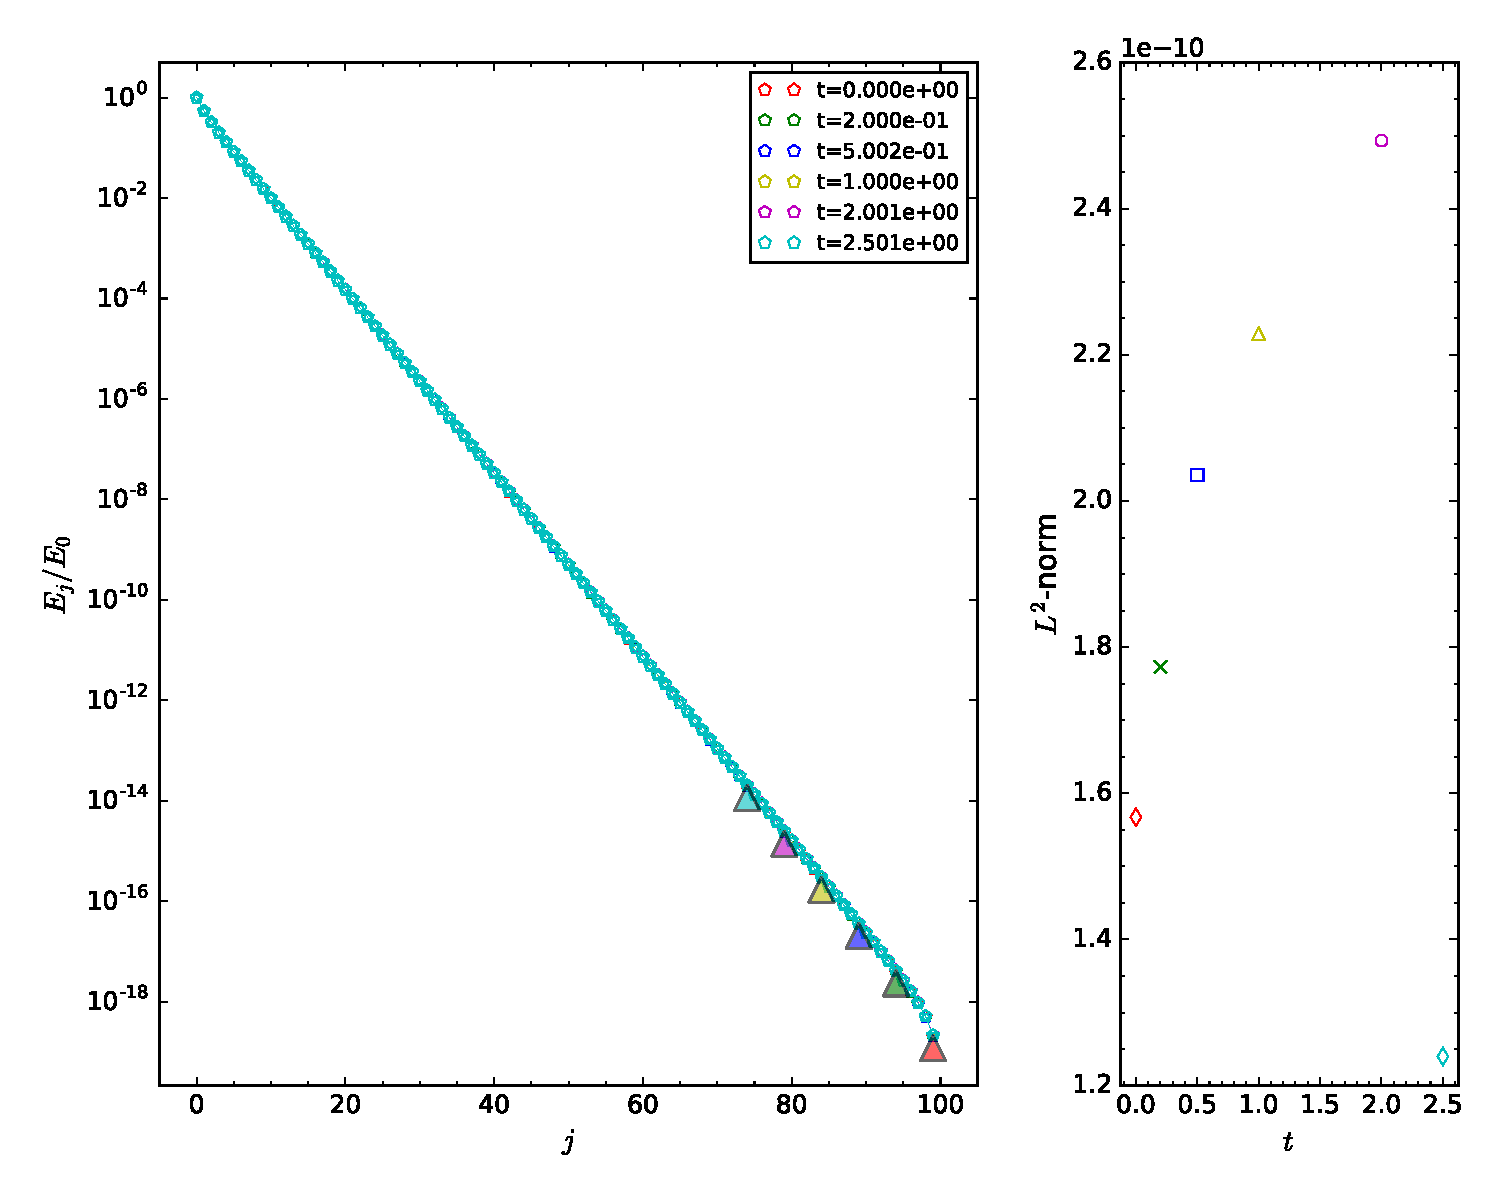
\includegraphics[width=\textwidth]{/Users/bradc/Research/Thesis/PhD/Chapter2/figs/Qpa4_40e-01j100EvolutionProjectionPlot}
		\caption{Projected solutions for a low-temperature, QP solution and their $L^2$-norms at $t\simeq 0.0, 0.2, 0.5, 1.0, 2.0, 2.5$ (red diamond, green cross, blue square, yellow triangle, magenta circle, blue diamond).}
		\label{fig: Qpa4_40e-01j100EvolutionProjection}
	\end{subfigure}
	\;
	\begin{subfigure}[t]{0.45\textwidth}
		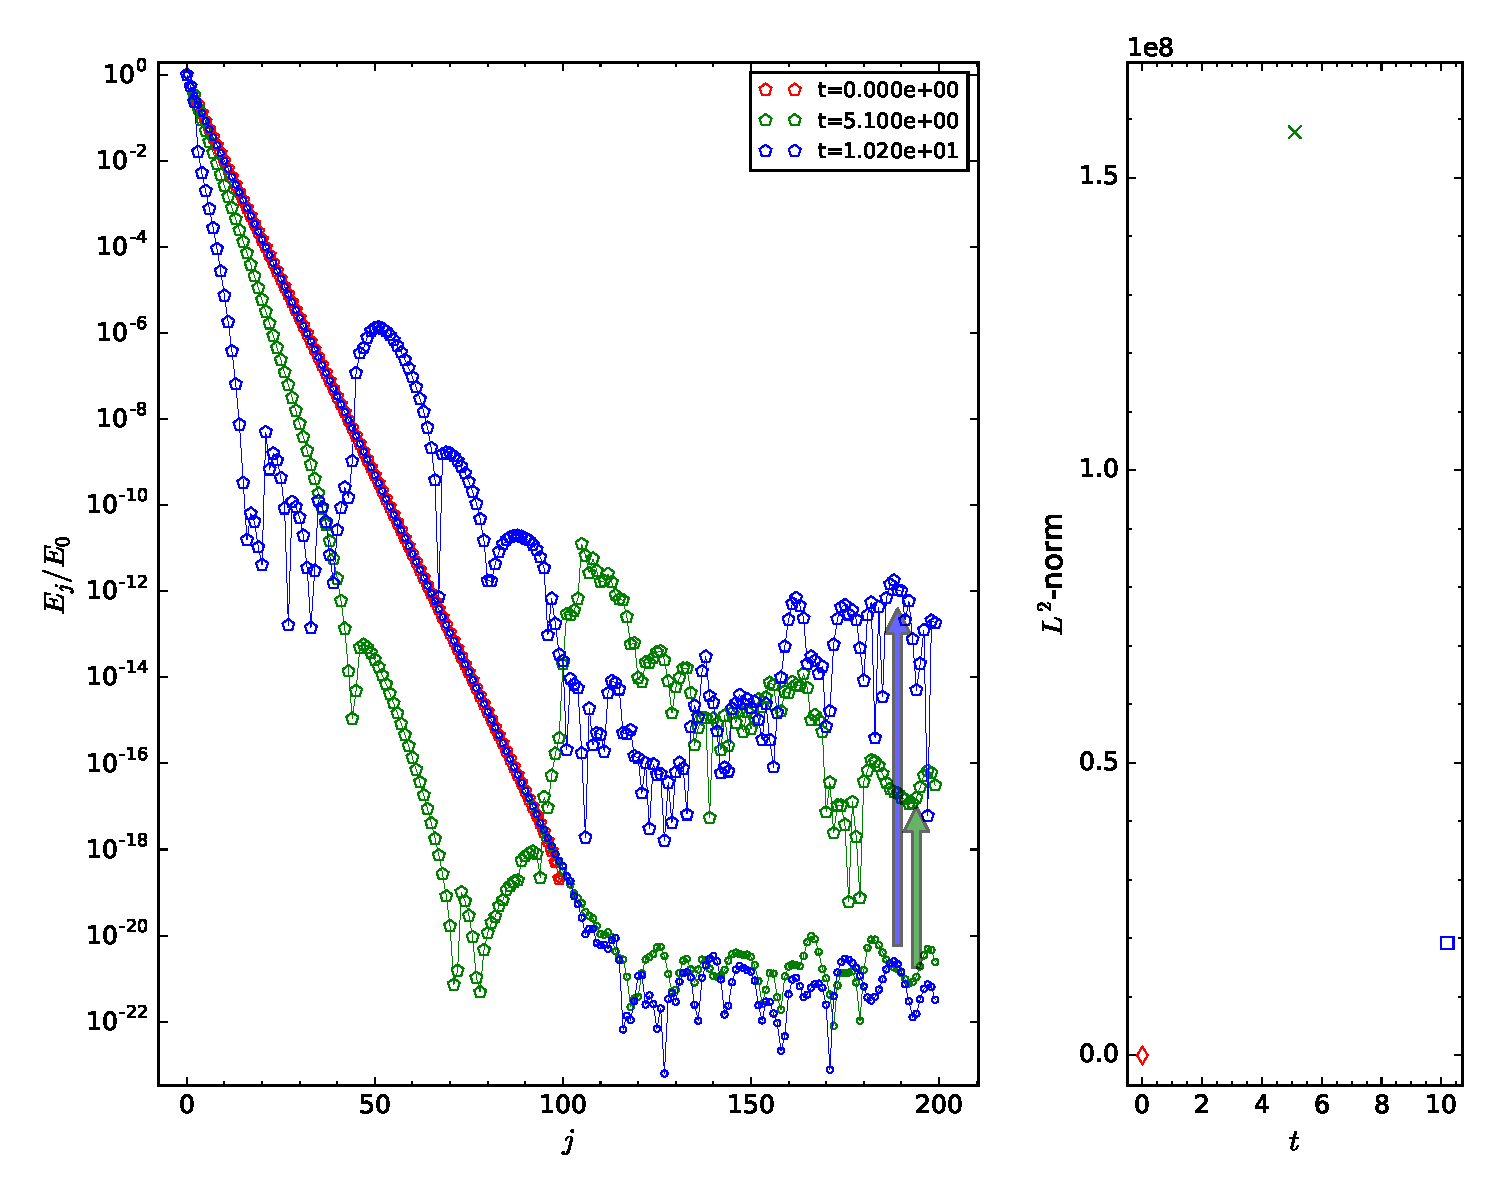
\includegraphics[width=\textwidth]{/Users/bradc/Research/Thesis/PhD/Chapter2/figs/QPa4_40e-01padj200_evolutionprojection}
		\caption{The same QP solution is padded with zeros out to $\jm = 200$ and evolved in time. Intermediate solutions are projected back to the QP plane at $t \simeq 0.0, 5.1, 10.2, ...$ (red diamond, green cross, blue square ...)}
		\label{fig: QPa4_40e-01padj200_evolutionprojection}
	\end{subfigure}
	\caption[Taking the spectrum of a QP solution during evolution to use as a seed to find new QP solutions]{Intermediate values from the amplitude/phase evolution of a solution are used as seeds for the nonlinear solver at various times. Arrows are oriented from amplitude/phase seed values (circles) to QP plane projections (pentagons).}
\end{figure}

%%%%%%%%%%%%%%%%%%%%%%%%%%%%%%%%%%%%%%%%%

\subsection{Padded QP Solutions}

In an effort to extend the space of QP solutions, another method used to find solutions that exist nearby known QP solutions -- but are not accessible through perturbative or conventional seeding methods -- is to pad a given quasi-periodic solution with extra modes that are initially set to zero. Upon amplitude-phase evolution, the energy in the lower-$j$ modes will flow into the higher-$j$ modes and a new quasi-periodic solution may be found. In figure~\ref{fig:paddedqpevo}, we construct initial data out of a known $\jm = 100$, $T \simeq 3.14$ solution by padding with zeros up to $\jm = 200$. As in the case of unpadded QP solution, the fraction of the total energy in the first four modes does not vary during the evolution and the highest modes accumulate some numerical error before levelling off. In figure~\ref{fig: paddedqp_fullspecevo}, we see the accumulation of numerical error in the higher modes as the evolution progresses. Also included is the value of the Ricci scalar at the origin, and the residuals of the QP equation throughout the evolution.

\begin{figure}[h]
	\centering
	\begin{subfigure}[t]{0.45\textwidth}
		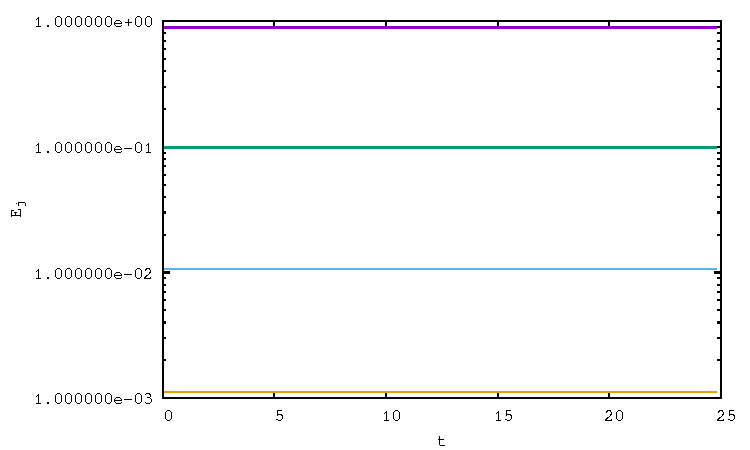
\includegraphics[width=\textwidth]{/Users/bradc/Research/Thesis/PhD/Chapter2/figs/paddedQPa2_00e-01_j200_lowjenergyevo}
		\caption{The evolution of the first four modes of the padded QP solution: $j=0,1,2,3$ (purple, green, blue, orange).}
	\end{subfigure}
	\;
	\begin{subfigure}[t]{0.45\textwidth}
		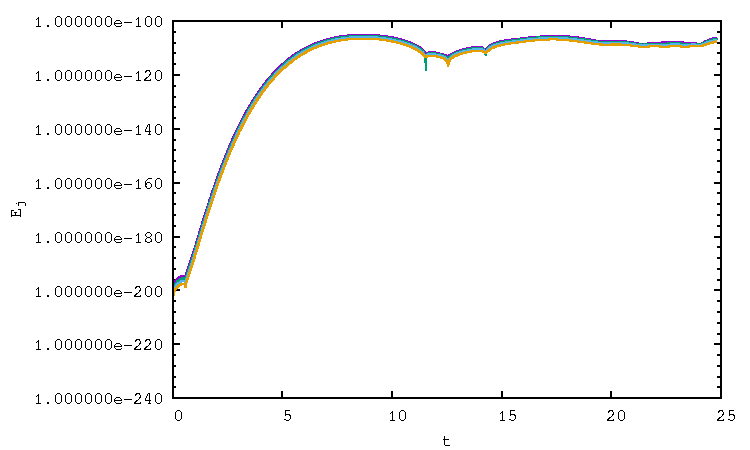
\includegraphics[width=\textwidth]{/Users/bradc/Research/Thesis/PhD/Chapter2/figs/paddedQPa2_00e-01_j200_highjenergyevo}
		\caption{The evolution of the last four modes: $j = 196, 197, 198, 199$ (purple, green, blue, orange).}
	\end{subfigure}
	\;
	\begin{subfigure}[t]{0.45\textwidth}
		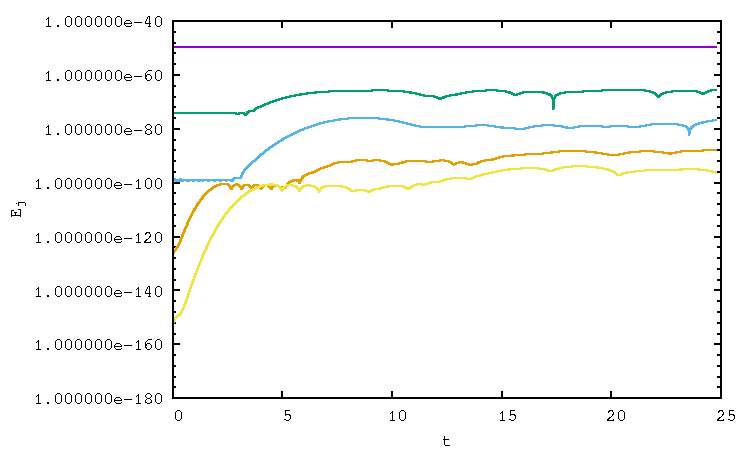
\includegraphics[width=\textwidth]{/Users/bradc/Research/Thesis/PhD/Chapter2/figs/paddedQPa2_00e-01_j200_energyevo}
		\caption{Comparing the evolution of a selection of modes: $j= 50, 75, 100, 125, 150$ (purple, green, blue, orange, yellow).}
	\end{subfigure}
	\;
	\begin{subfigure}[t]{0.45\textwidth}
		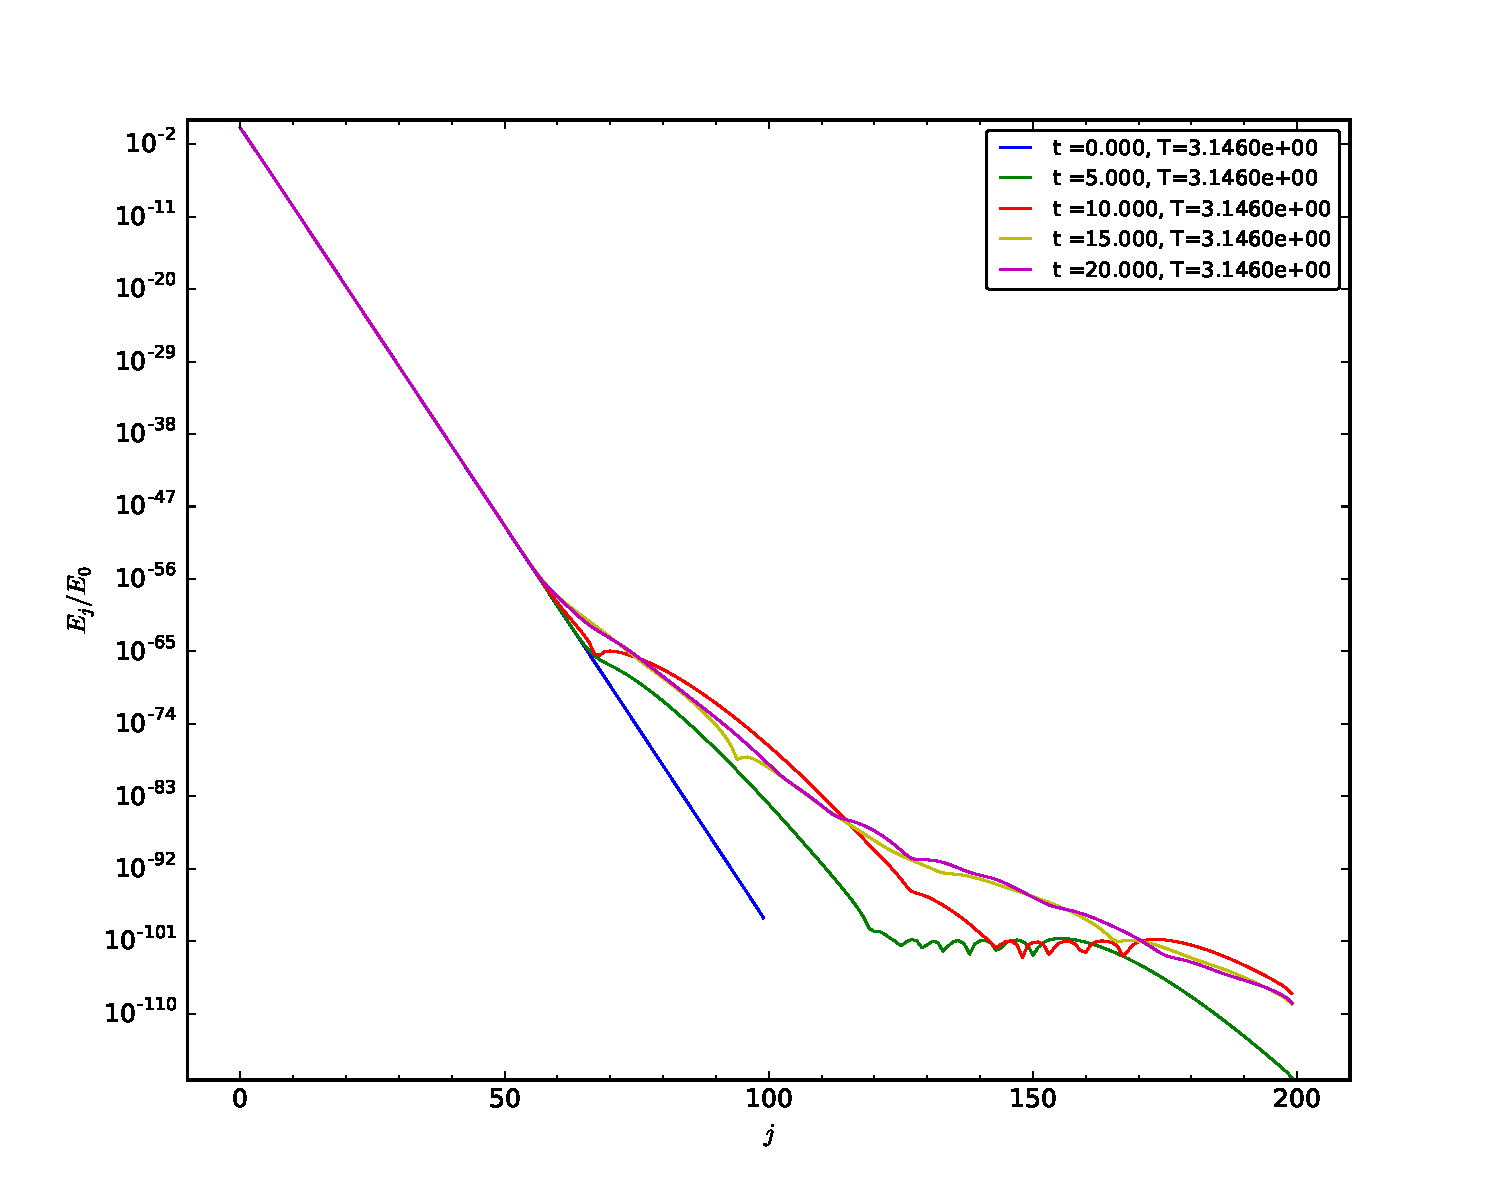
\includegraphics[width=\textwidth]{/Users/bradc/Research/Thesis/PhD/Chapter2/figs/paddedQPa2_00e-01_j200_spectrumevo}
		\caption{The total spectrum of the padded QP solution as a function of time.}
		\label{fig: paddedqp_fullspecevo}
	\end{subfigure}
	\;
	\begin{subfigure}[t]{0.45\textwidth}
		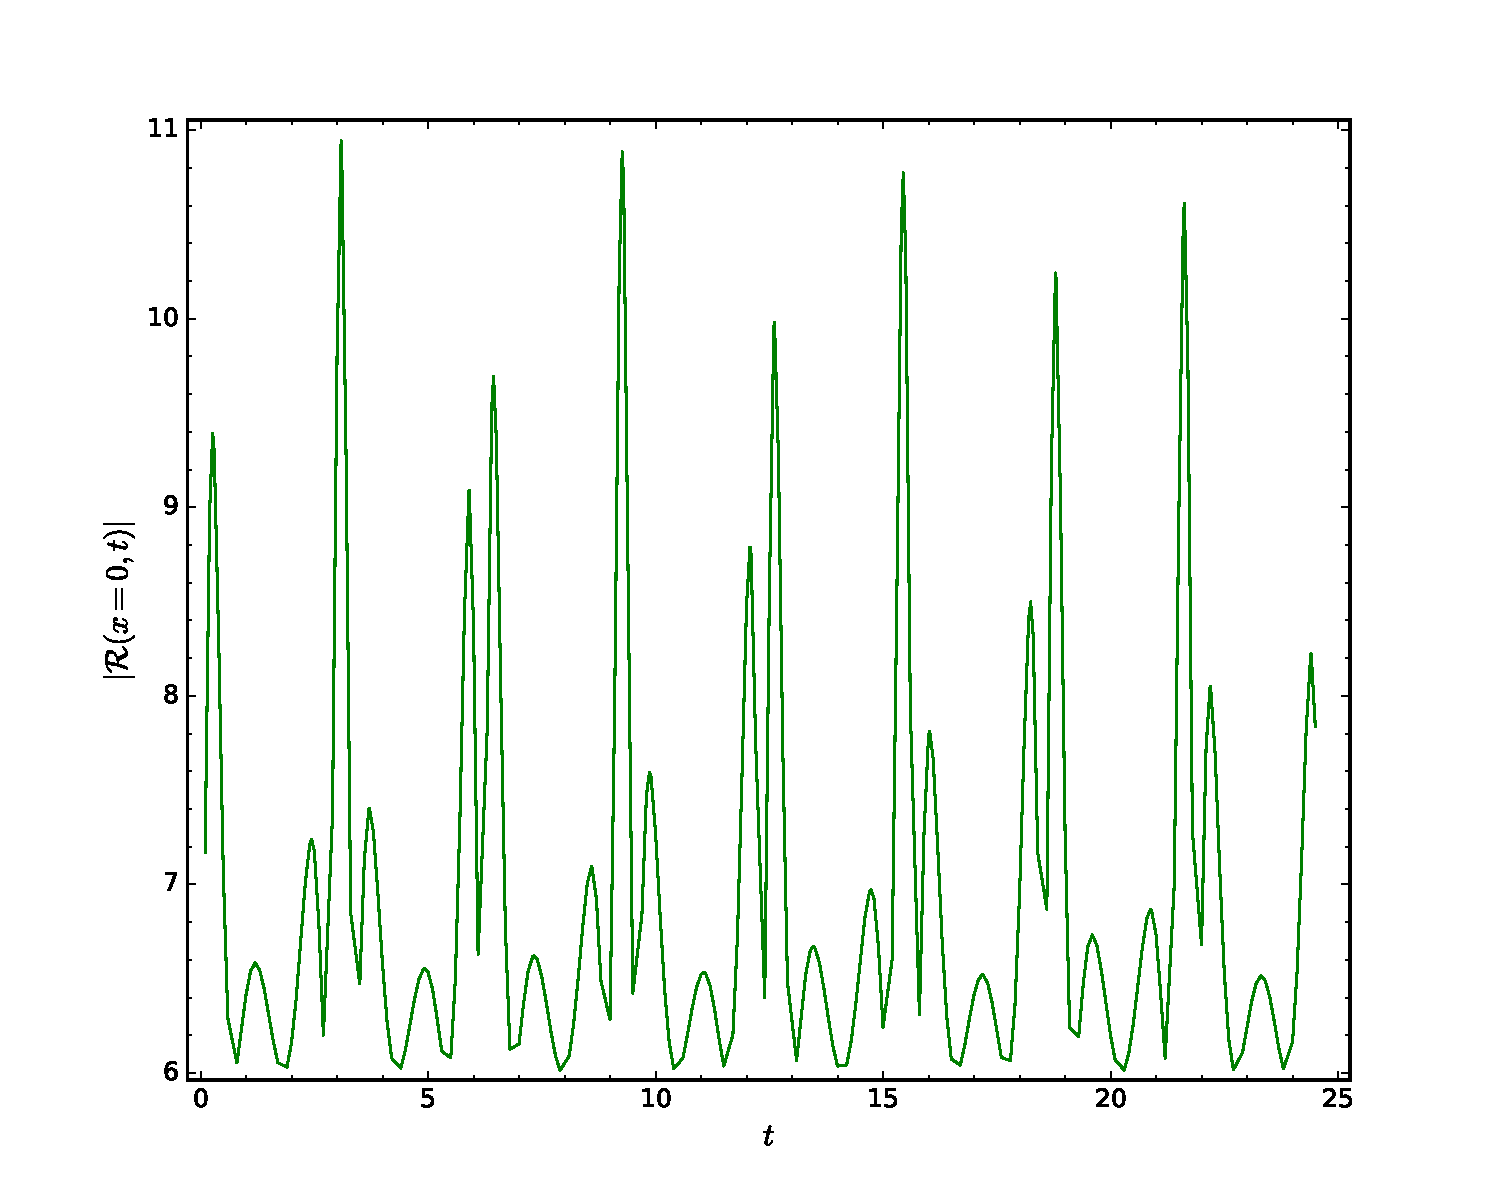
\includegraphics[width=\textwidth]{/Users/bradc/Research/Thesis/PhD/Chapter2/figs/Qpa2_00e-01padj200_ricci}
		\caption{The Ricci scalar at the origin as a function of time for the padded QP solution.}
	\end{subfigure}
	\;
	\begin{subfigure}[t]{0.45\textwidth}
		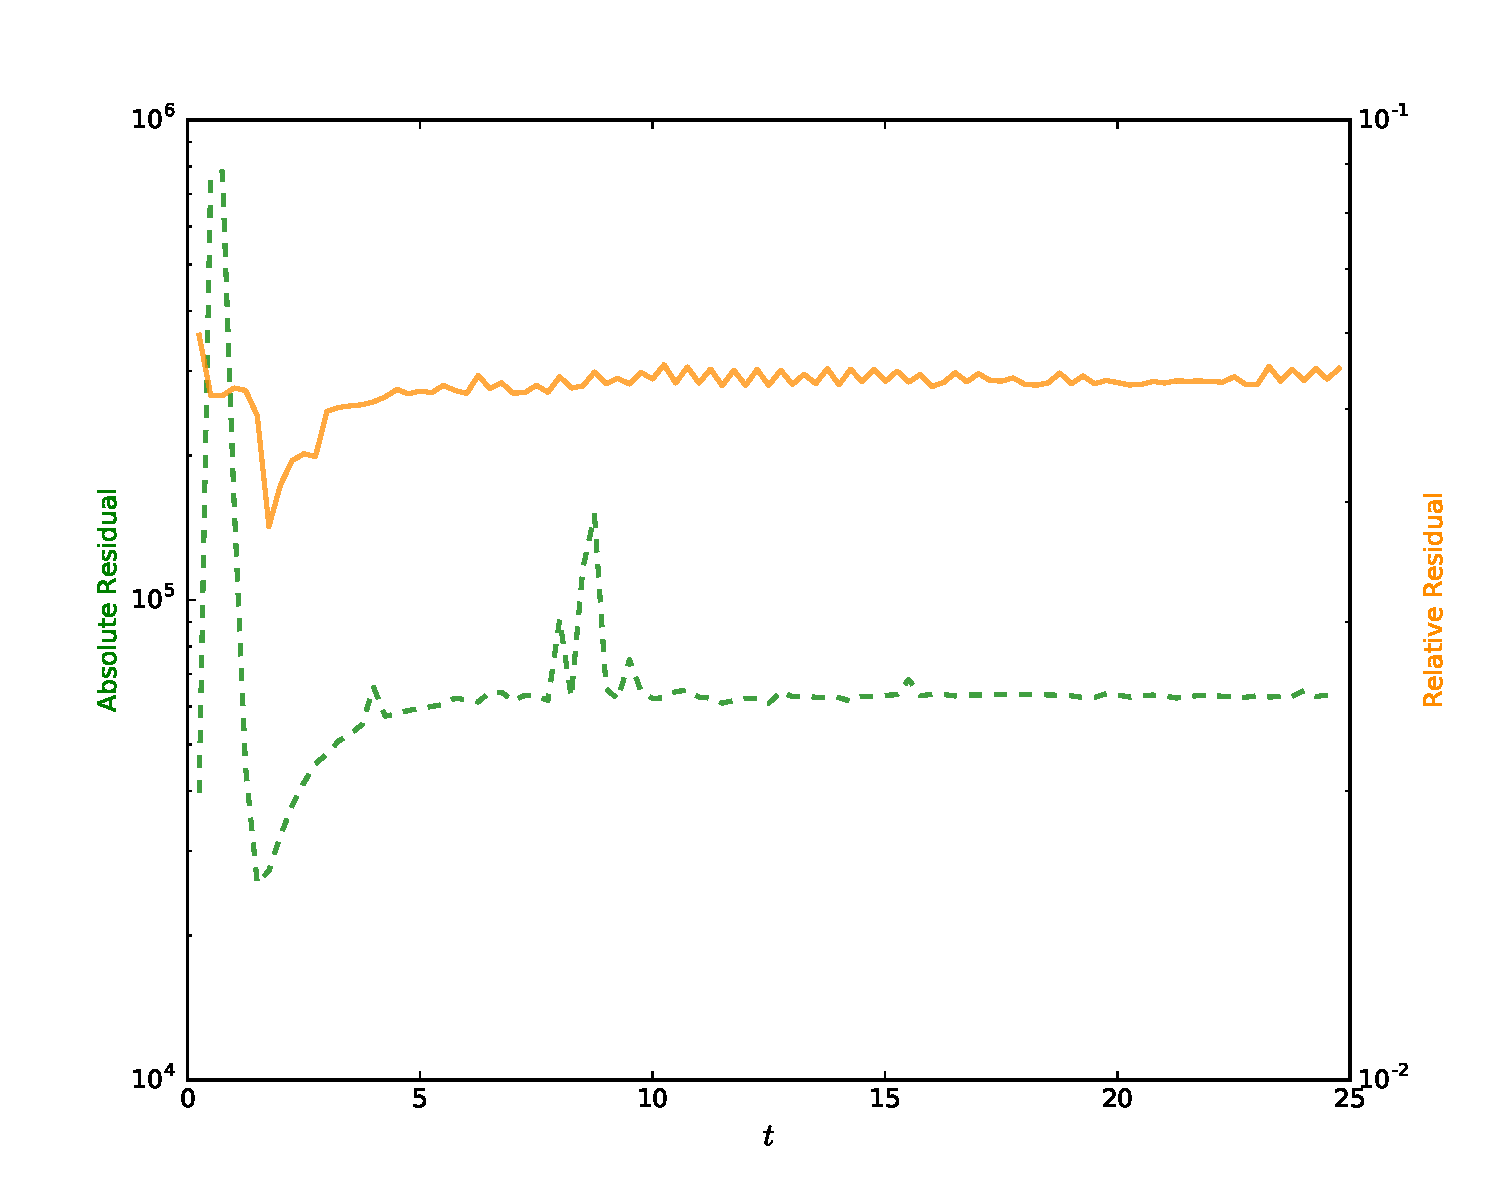
\includegraphics[width=\textwidth]{/Users/bradc/Research/Thesis/PhD/Chapter2/figs/Qp2_00e-01padj200_resids}
		\caption{The residuals of the QP equation \eqref{qp eqn} throughout the amplitude-phase evolution of the padded QP solution.}
		\label{fig: Qp2_00e-01padj200_resids}
	\end{subfigure}
	\caption[The evolution of a padded QP solution]{The evolution of the padded QP solution for $\alpha_1 =0.2$ and $\jm = 200$, with amplitude $\epsilon=0.1$.}
	\label{fig:paddedqpevo}
\end{figure}

Despite the somewhat normal profile of the spectra of padded QP solution, we see in figure~\ref{fig: QPa4_40e-01padj200_evolutionprojection} that intermediate solutions during the evolution in fact \emph{do not} project back to the QP plane. Rather, as hinted at by the Einstein equation residuals shown in figure~\ref{fig: Qp2_00e-01padj200_resids}, the solutions have drifted away from their quasi-periodic initial data. It remains to be seen whether such profiles would be stable in the fully nonlinear system.

Using a known QP solution, we may ask how far away from the solution plane we can move by padding with an incremental number of zeros. In figure~\ref{fig: Qpa2_00e-01padj105_evolutionprojection}, we show the result of using intermediate solutions from the amplitude/phase evolution of a $\jm = 100$ QP solution padded with only five modes (initially set to zero). Despite QP solutions existing for $\jm = 105$, no solution was found when using the padded solution -- at any point in its evolution -- as a seed.

%\begin{figure}[ht]
%	\centering
%	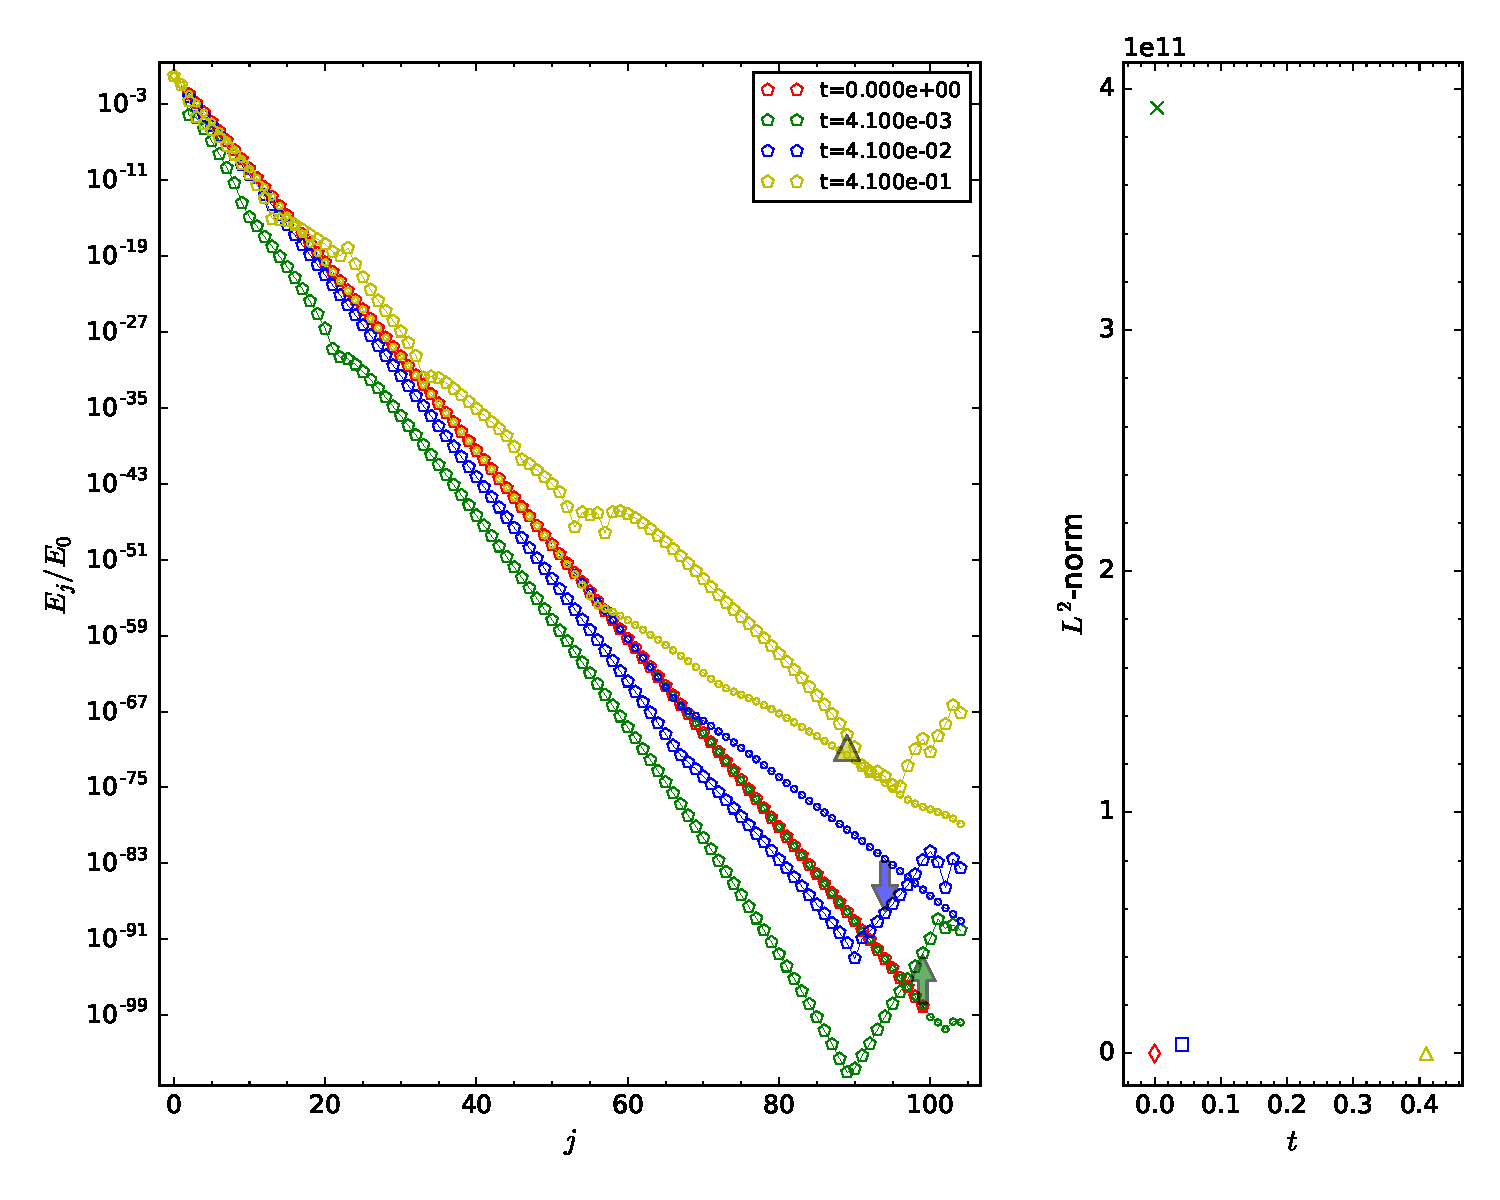
\includegraphics[width=0.75\textwidth]{/Users/bradc/Research/Thesis/PhD/Chapter2/figs/Qpa2_00e-01padj105_evolutionprojection}
%	\caption[Spectra during evolution of a padded QP solution are used as seeds to project back to the QP plane]{{\it Left}: Normalized spectra for a $\jm = 100$, QP solution that has been padded with five extra modes, then evolved in time. Intermediate spectra are used as seeds for projecting back to the QP plane at times $\tau \simeq 4.1 \times 10^{-3}, 4.1 \times 10^{-2}, 4.1 \times 10^{-1}$ (green, blue, yellow). Arrows are oriented from seed spectra to best fit spectra. {\it Right:} Corresponding $L^2$-norms of the error for each solution.}
%	\label{fig: Qpa2_00e-01padj105_evolutionprojection}
%\end{figure}

%%%%%%%%%%%%%%%%%%%%%%%%%%%%%%%%%%%%%%%%%

\subsection{High-Temperature Solutions}

High-temperature solutions are those that are found by repeated applications of energy perturbations described in \S\!~\ref{ssec: highT}. These come in several varieties based on the methods used to obtain them; namely, the frequency of projection back to the QP solution plane versus constructing solutions ``by hand.'' Note that solutions obtained without projecting back to the QP plane, or via the threshold temperature method, \emph{are not} robust in the limit of large $\jm$ (see Appendix~\ref{app: reop freq} for further discussion on the extension of high-temperature solutions to large $\jm$). However, it will be useful nonetheless to contrast their behaviour with other high-temperature solutions.

%%%%%%%%%%%%%%%%%%%%%%%%%%%%%%%%%%%%%%%%%

\subsection{Regular Projections to the QP Plane}
\label{sssec: evo of regular projections}

Here we examine a high-temperature solution obtained from repeatedly adding small amounts of energy to a $\jm = 100$, $\alpha_1 = 0.44$ QP solution. First, we consider threshold temperature solutions discussed in \S~\!\ref{ssec: highT} -- those that are on the cusp of quasi-periodic data but cannot be found through solving \eqref{qp eqn} alone. See figure~\ref{fig:HighTa4_072e-01j100T5_3921e+00_evo} for results.

\begin{figure}[h]
	\centering
	\begin{subfigure}[t]{0.48\textwidth}
		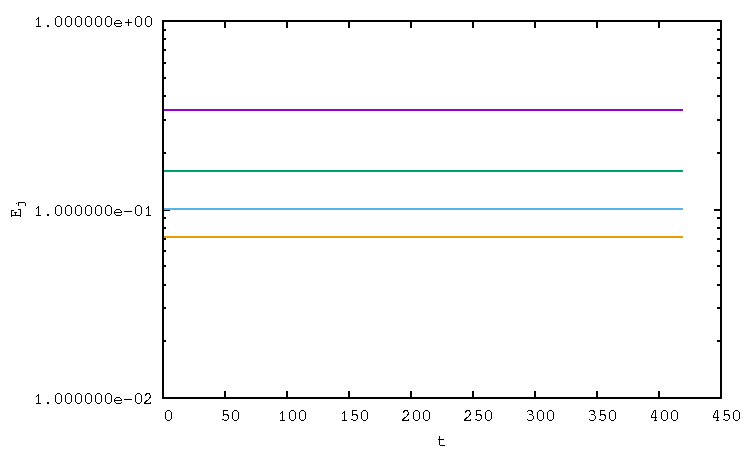
\includegraphics[width=\textwidth]{/Users/bradc/Research/Thesis/PhD/Chapter2/figs/HighTa4_072e-01j100T5_3921e+00_lowjevo}
		\caption{$j = 0, 1, 2, 3$ (purple, green, blue, orange).}
	\end{subfigure}
	\;
	\begin{subfigure}[t]{0.48\textwidth}
		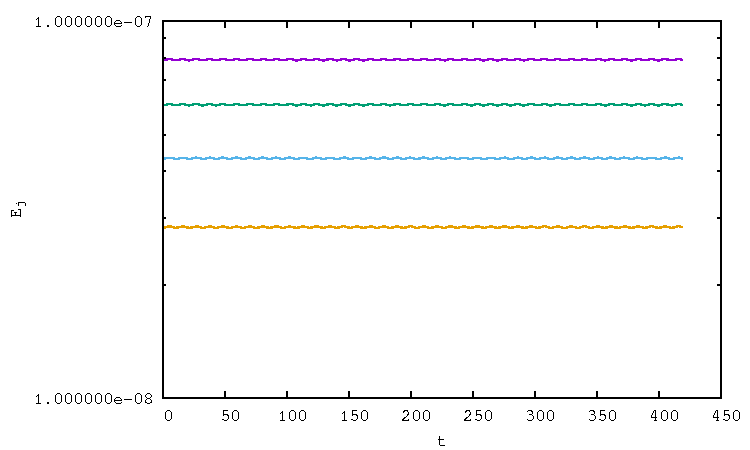
\includegraphics[width=\textwidth]{/Users/bradc/Research/Thesis/PhD/Chapter2/figs/HighTa4_072e-01j100T5_3921e+00_highjevo}
		\caption{$j=96, 97, 98, 99$ (purple, green, blue, orange).}
		\label{fig: HighTa4_072e-01j100T5_3921e+00_highjevo}
	\end{subfigure}
	\\
	\begin{subfigure}[t]{0.48\textwidth}
		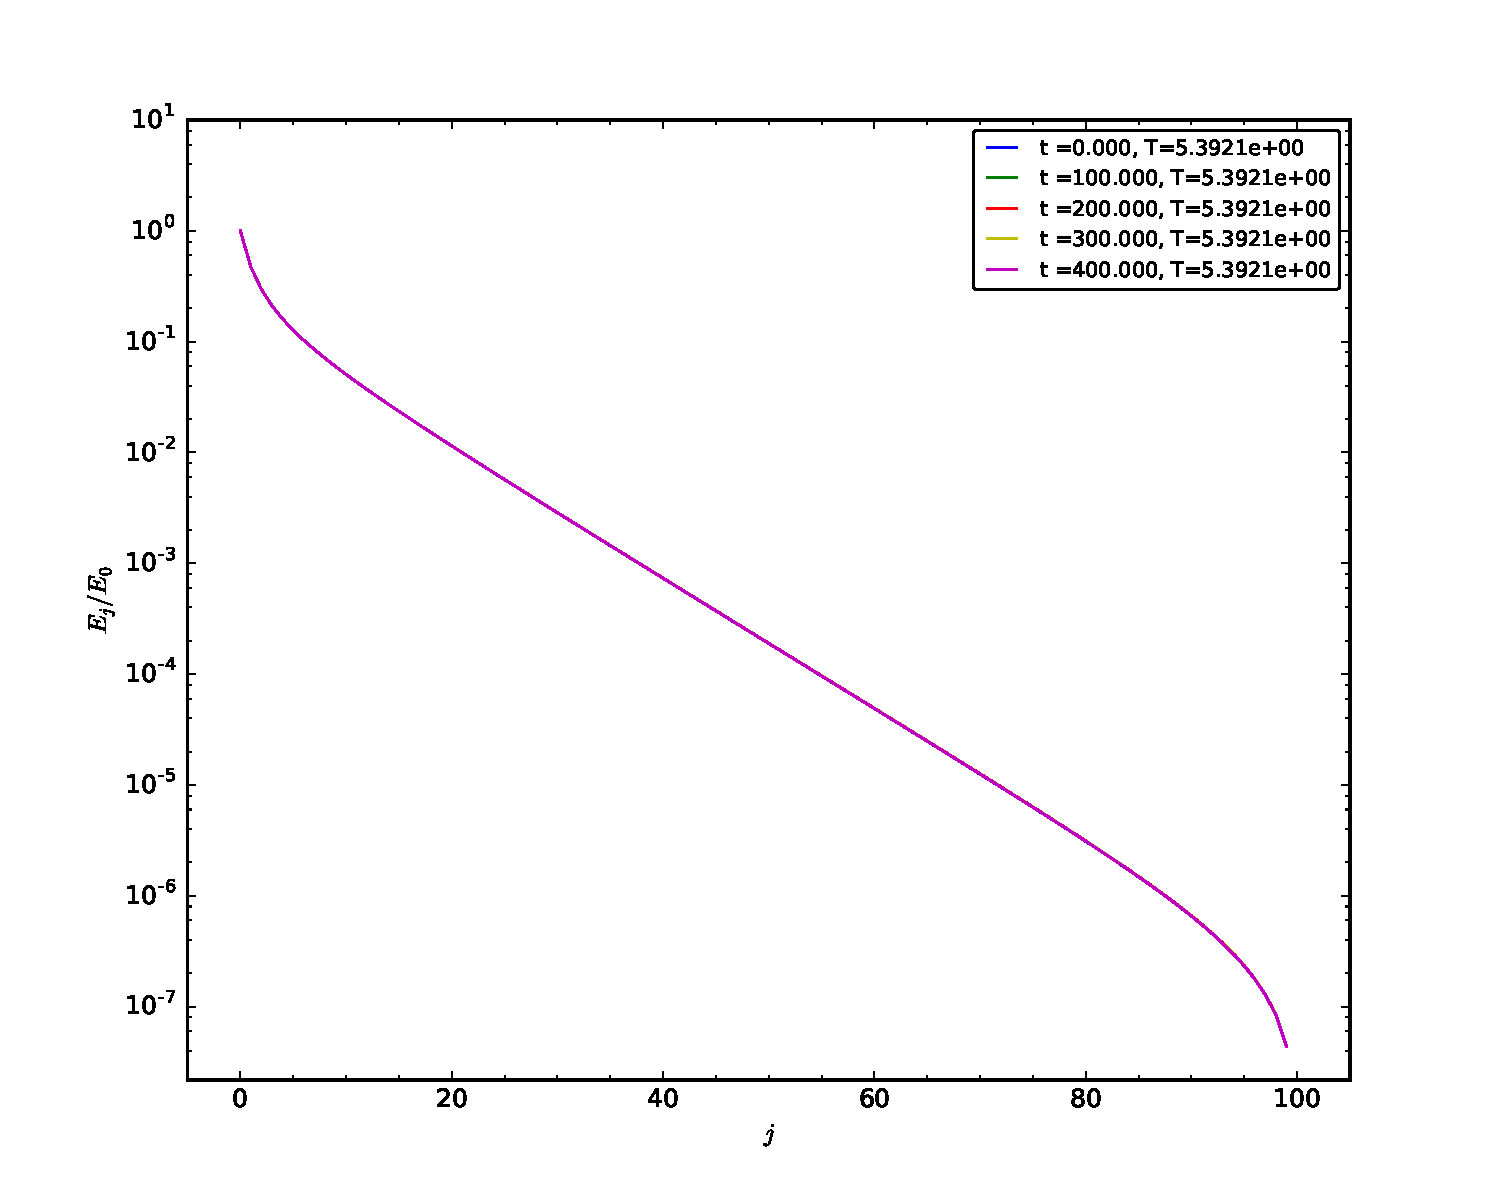
\includegraphics[width=\textwidth]{/Users/bradc/Research/Thesis/PhD/Chapter2/figs/HighTa4_072e-01j100T5_3921e+00_spectrumevo}
	\end{subfigure}
	\quad
	\begin{subfigure}[t]{0.48\textwidth}
		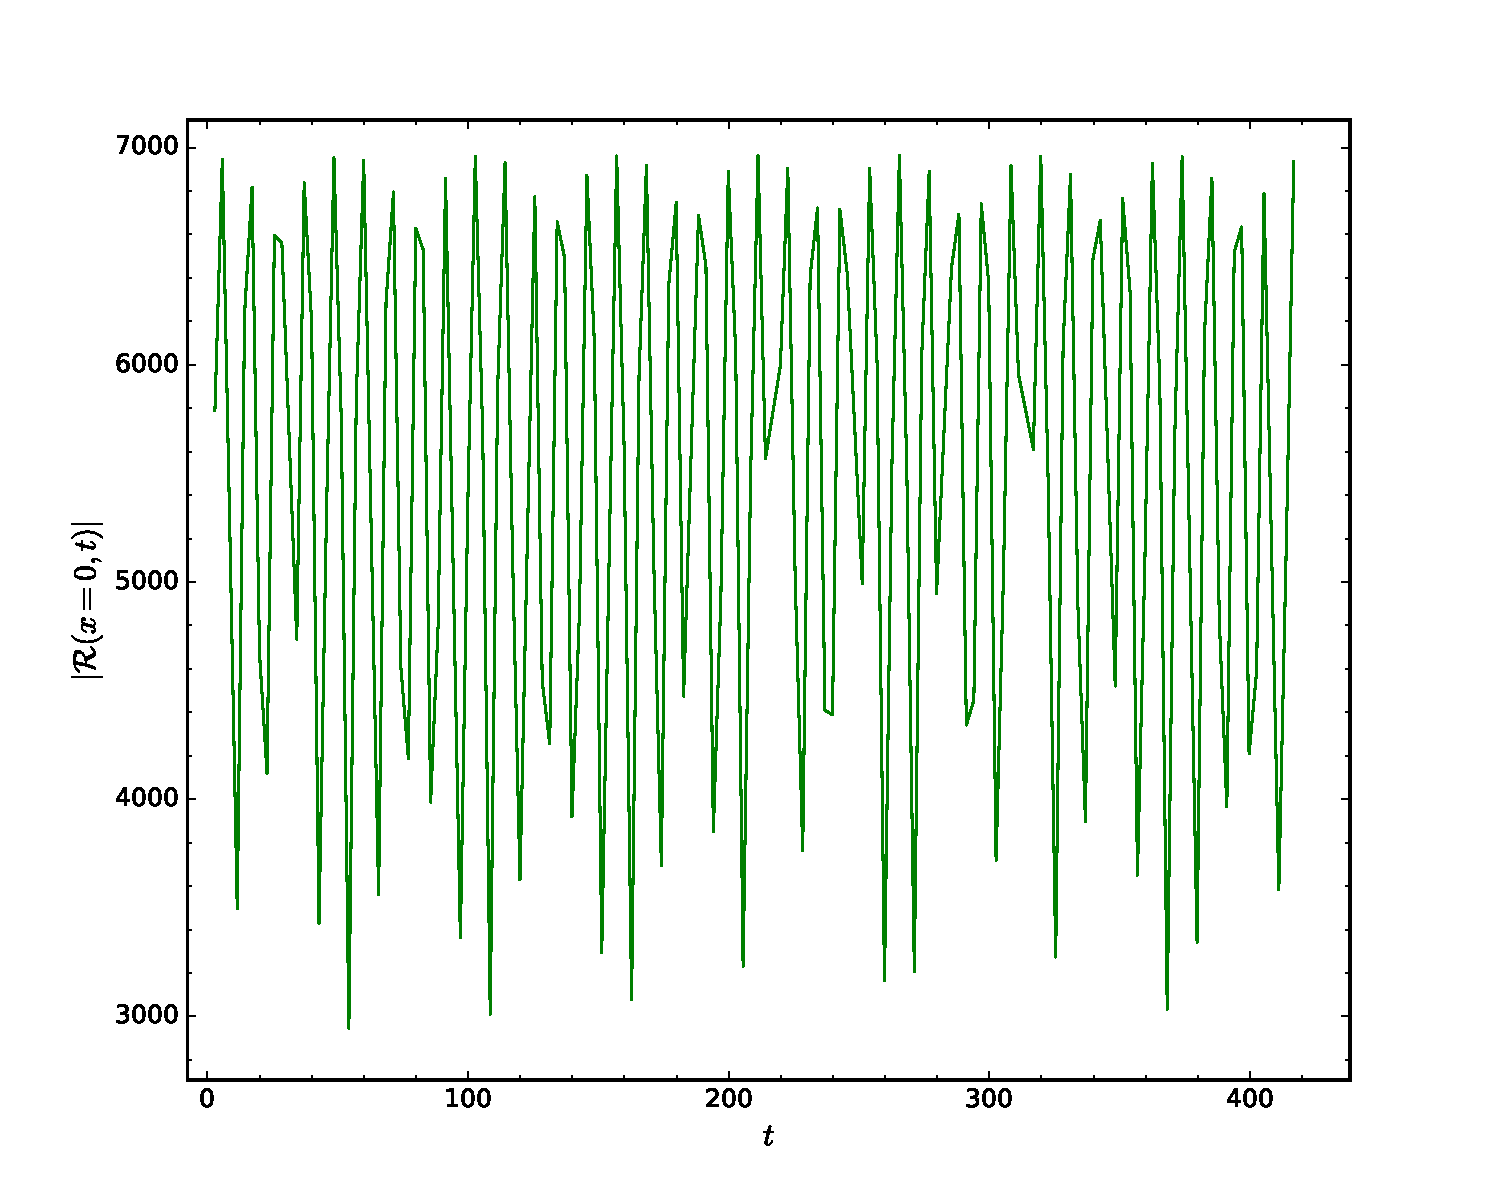
\includegraphics[width=\textwidth]{/Users/bradc/Research/Thesis/PhD/Chapter2/figs/HighTa4_072e-01j100T5_3921e+00Ricci}
	\end{subfigure}
	\caption[Examining the energy per mode during the evolution of a threshold temperature solution]{{\it Above}: The evolution the fraction of the total energy in specific modes for a $T \sim 5.4$, threshold temperature solution for $\tau \in [0, 4.25]$. {\it Below:} Snapshots of the full spectrum at various times in its evolution, as well as the upper envelope of $| \mc R(t,x=0)|$ when $\epsilon = 0.1$.}
	\label{fig:HighTa4_072e-01j100T5_3921e+00_evo}
\end{figure}

Threshold temperature solutions behave much like low-temperature quasi-periodic solutions: no energy transfer occurs among the leading modes, while very little occurs in the highest modes. Note the scale in figure~\ref{fig: HighTa4_072e-01j100T5_3921e+00_highjevo}. Unlike other QP solutions with similar total number of modes, the highest modes in threshold temperature solutions contain $\mc O(10^{-7}) E_T $. This relatively high value of the fraction of the total energy means that numerical errors remain suppressed throughout the evolution.

%%%%%%%%%%%%%%%%%%%%%%%%%%%%%%%%%%%%%%%%%

\subsection{``By Hand'' High-Temperature Solutions}

Following the method outlined in \S~\!\ref{ssec: by hand highT}, we consider high-temperature solutions constructed by hand out of lower $\jm$ solutions. We now examine the behaviour of one such solution under amplitude-phase evolution. 

\begin{figure}[h!]
	\centering
	\begin{subfigure}[t]{0.45\textwidth}
		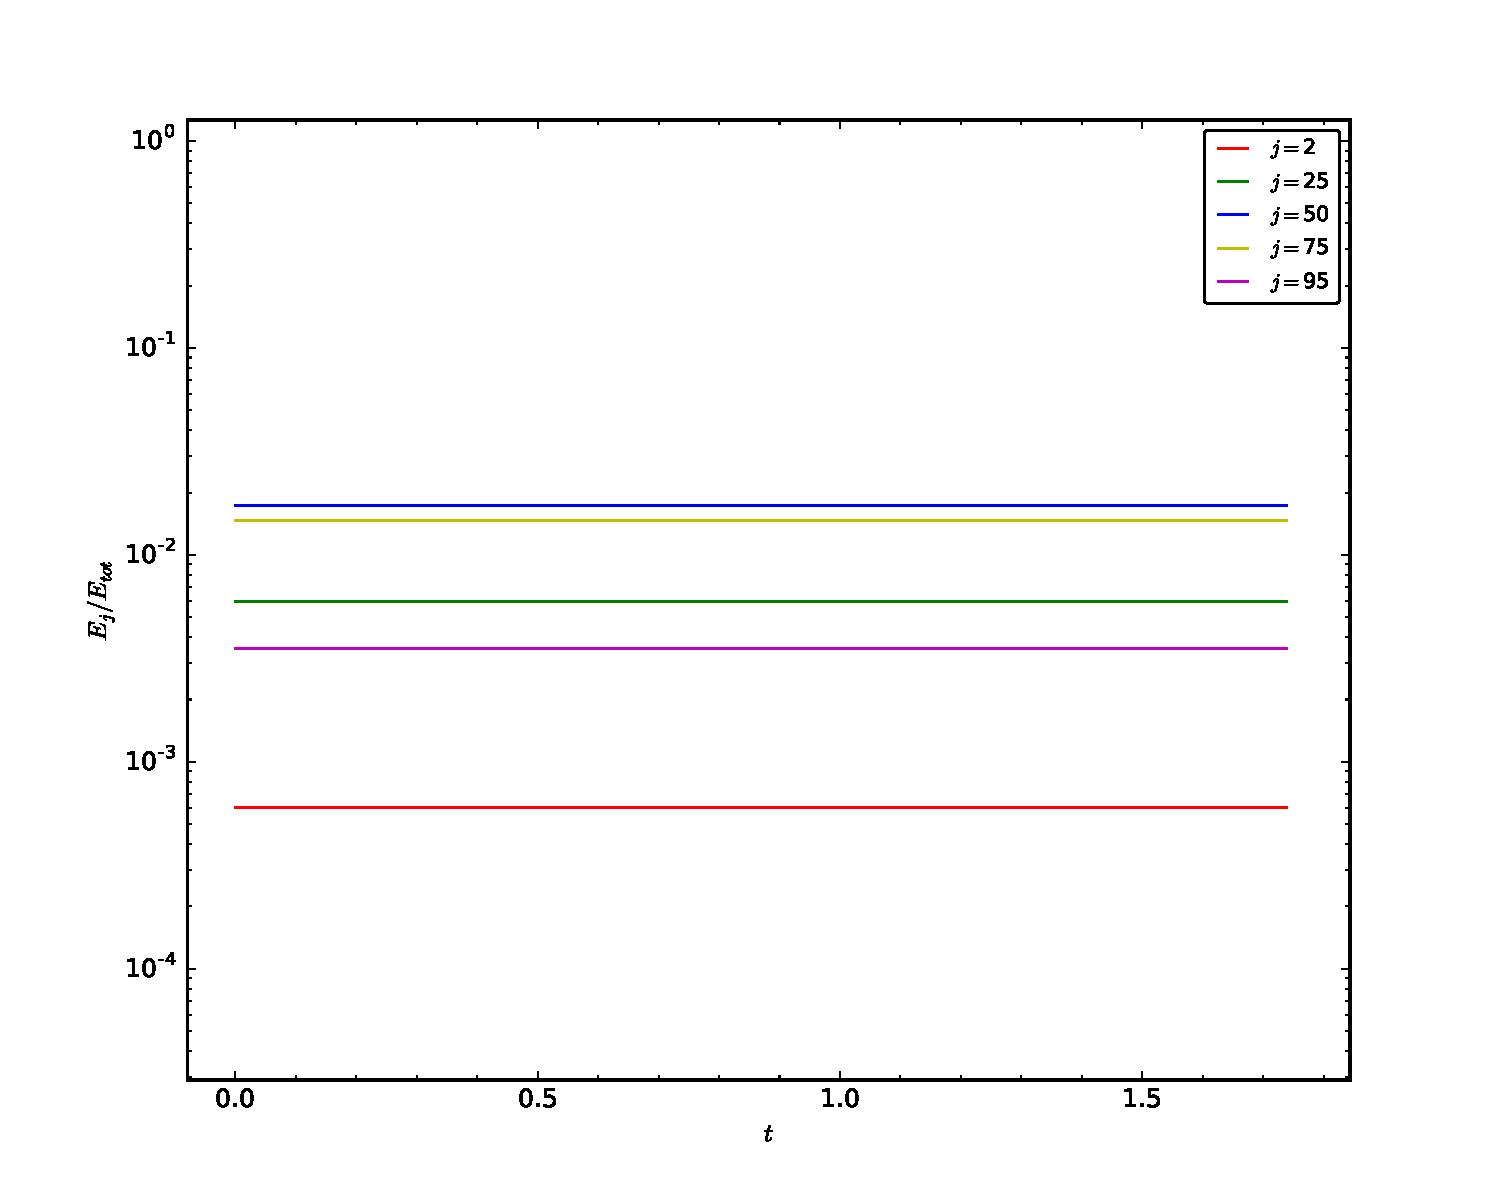
\includegraphics[width=\textwidth]{/Users/bradc/Research/Thesis/PhD/Chapter2/figs/HighTa2_1819e-01j100T6_6711e+01_fullevo}
	\end{subfigure}
	\;
	\begin{subfigure}[t]{0.45\textwidth}
		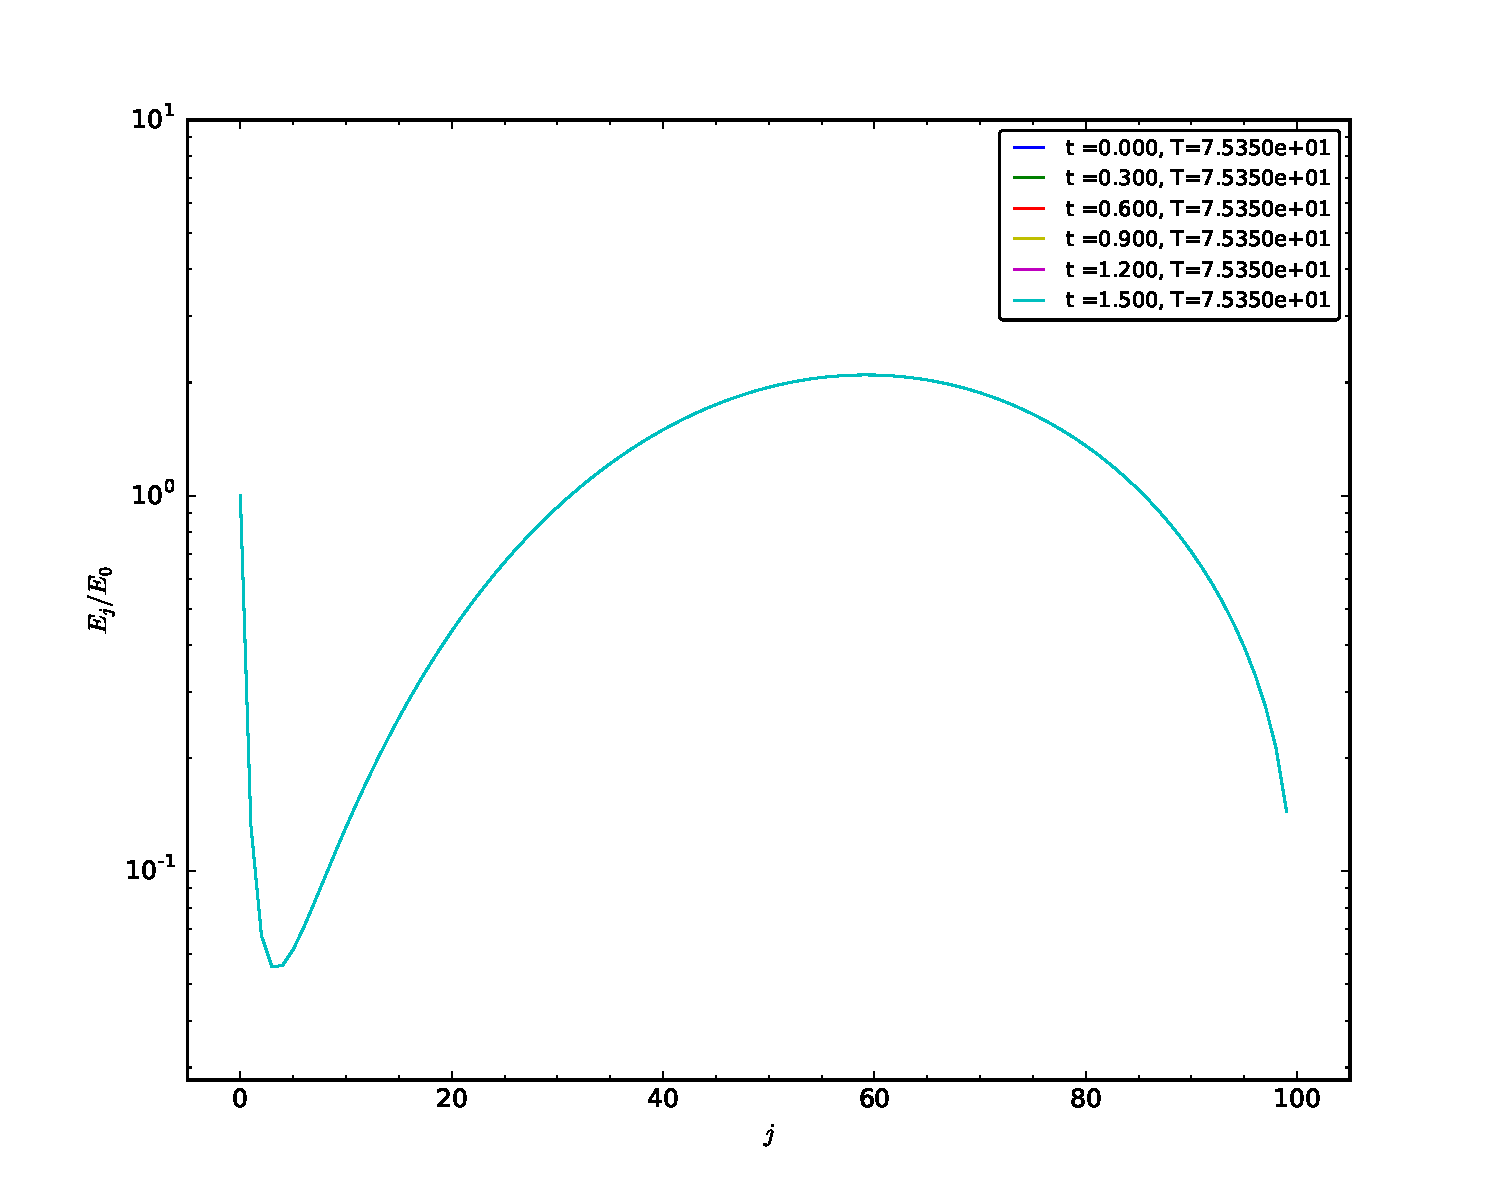
\includegraphics[width=\textwidth]{/Users/bradc/Research/Thesis/PhD/Chapter2/figs/HighTa2_1819e-01j100T6_6711e+01_specevo}
	\end{subfigure}
	\caption[Evolution of the energy spectrum for a high-temperature solution created by hand]{The evolution of a high-temperature solution created by hand from lower $\jm$ solutions.}
	\label{fig: HighTa2_1819e-01j100T6_6711e+01}
\end{figure}

Padding QP solutions with $T > T_{th}$ and evolving does not give sensible results: high relative residuals in QP equation.

\begin{figure}[h]
	\centering
	\begin{subfigure}[t]{0.45\textwidth}
		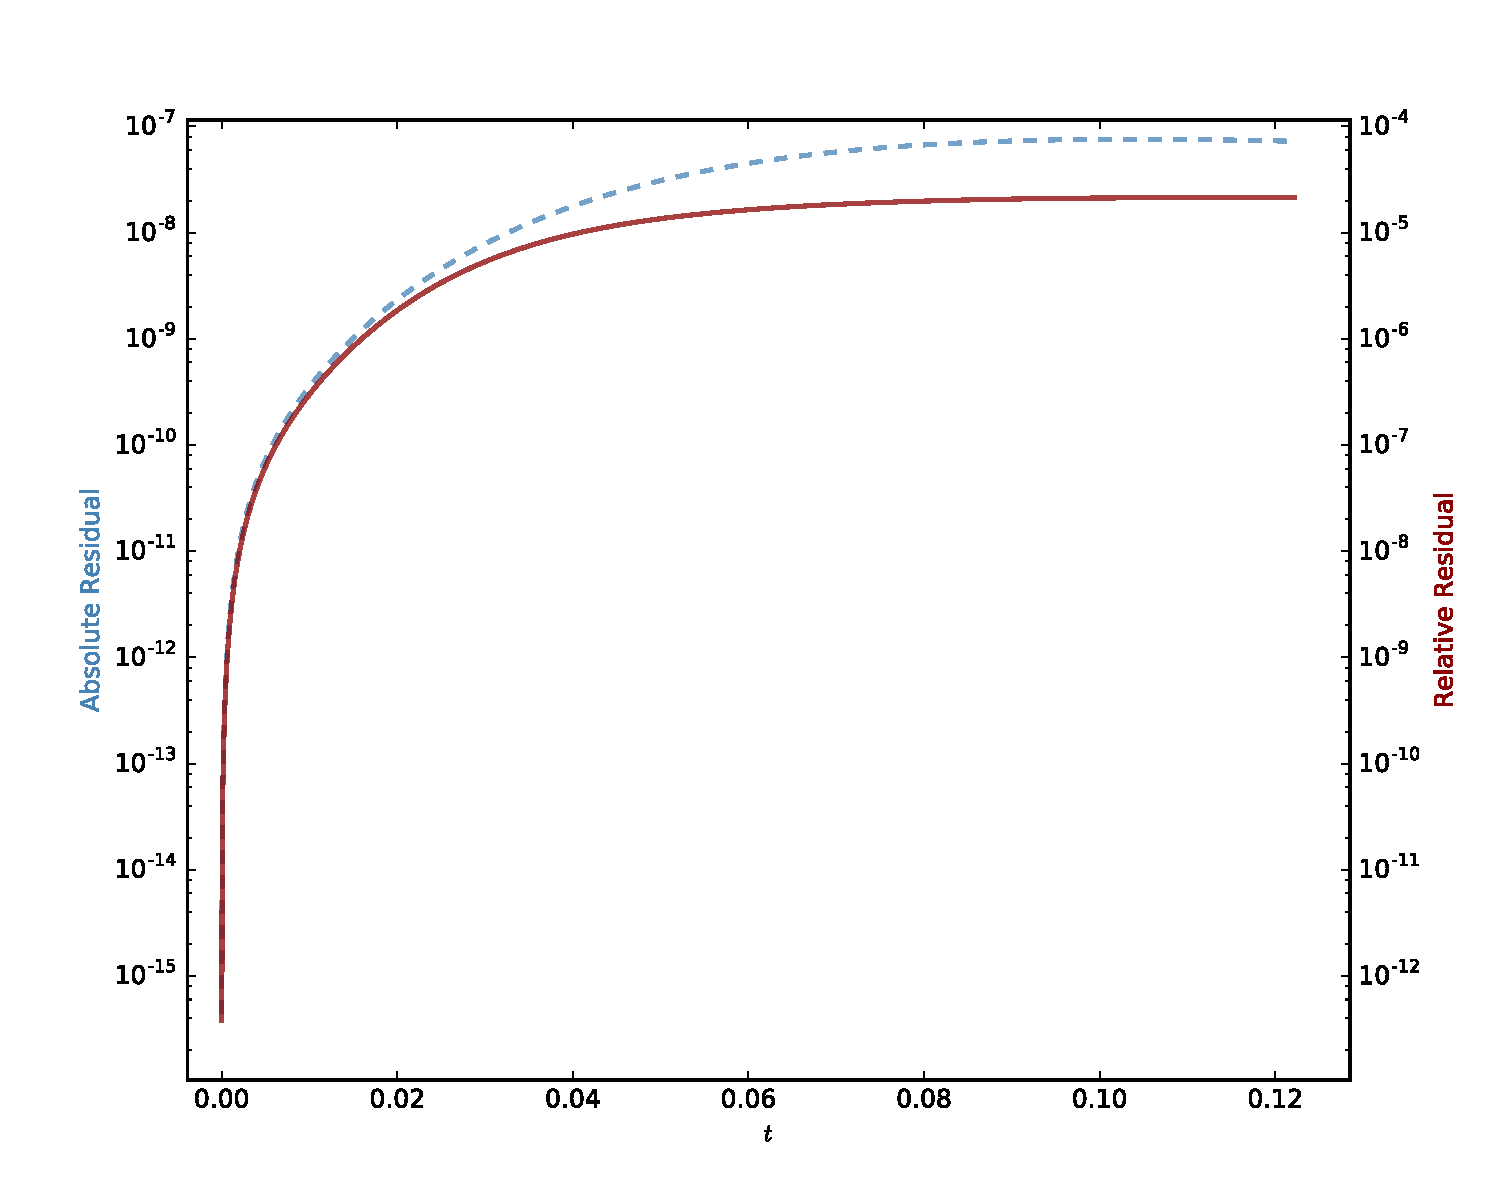
\includegraphics[width=\textwidth]{/Users/bradc/Research/Thesis/PhD/Chapter2/figs/Qpa4_40e-01j100EEresids}
		\caption{An $\alpha_1 = 0.44$, $\jm = 100$ QP solution with $\epsilon = 0.001$.}
		\label{fig:QPEEresid}
	\end{subfigure}
	\;
	\begin{subfigure}[t]{0.45\textwidth}
		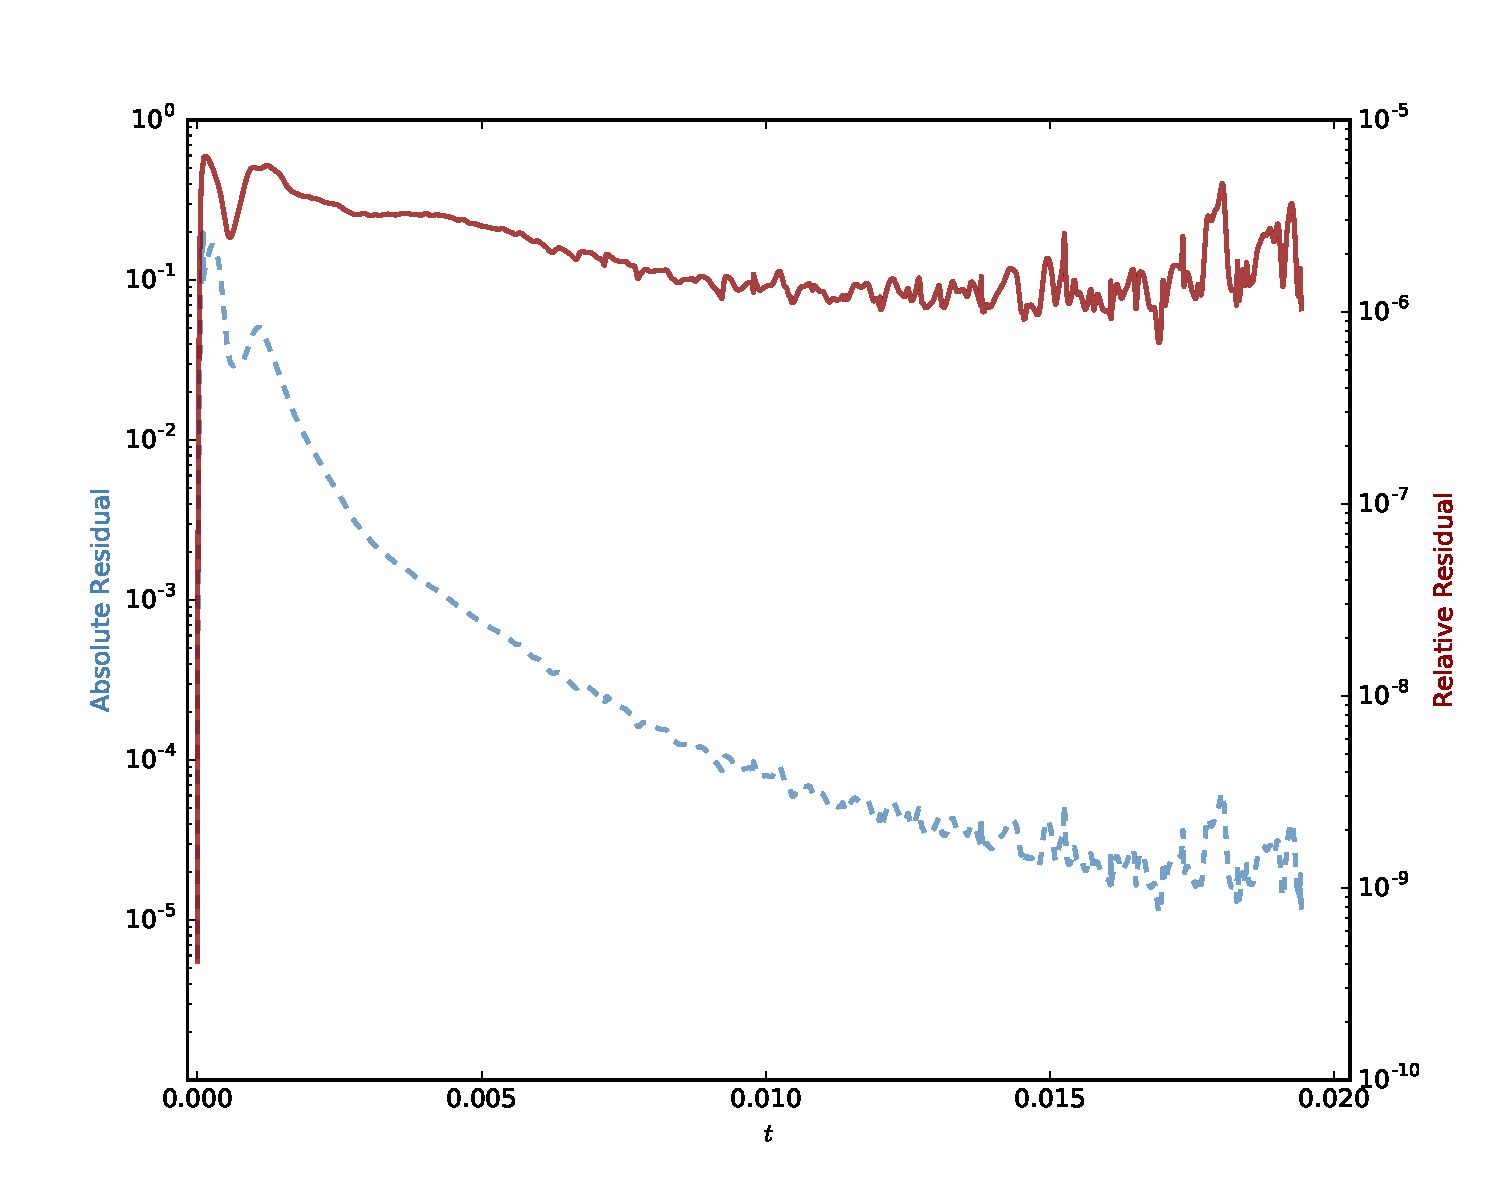
\includegraphics[width=\textwidth]{/Users/bradc/Research/Thesis/PhD/Chapter2/figs/HighTa2_1819e-01padj125T6_6711e+01_EEresids}
		\caption{A $\jm = 100$, high-temperature solution is padded with zeros to $\jm = 125$ and evolved with $\epsilon = 0.001$.}
		\label{fig:highTEEresid}
	\end{subfigure}
	\caption[Absolute and relative residuals for low- and high-temperature QP solutions]{Residuals from evaluating the constraints for QP and high temperature solutions.}
	\label{fig:EEresids}
\end{figure}




%Attempt padding out to $\jm = 125$ and run the evolution: see figure~\ref{fig:HighTa2_1819e-01padj125T6_6711e+01_evo}
%\begin{figure}[h]
%	\centering
%	\begin{subfigure}[t]{0.45\textwidth}
%		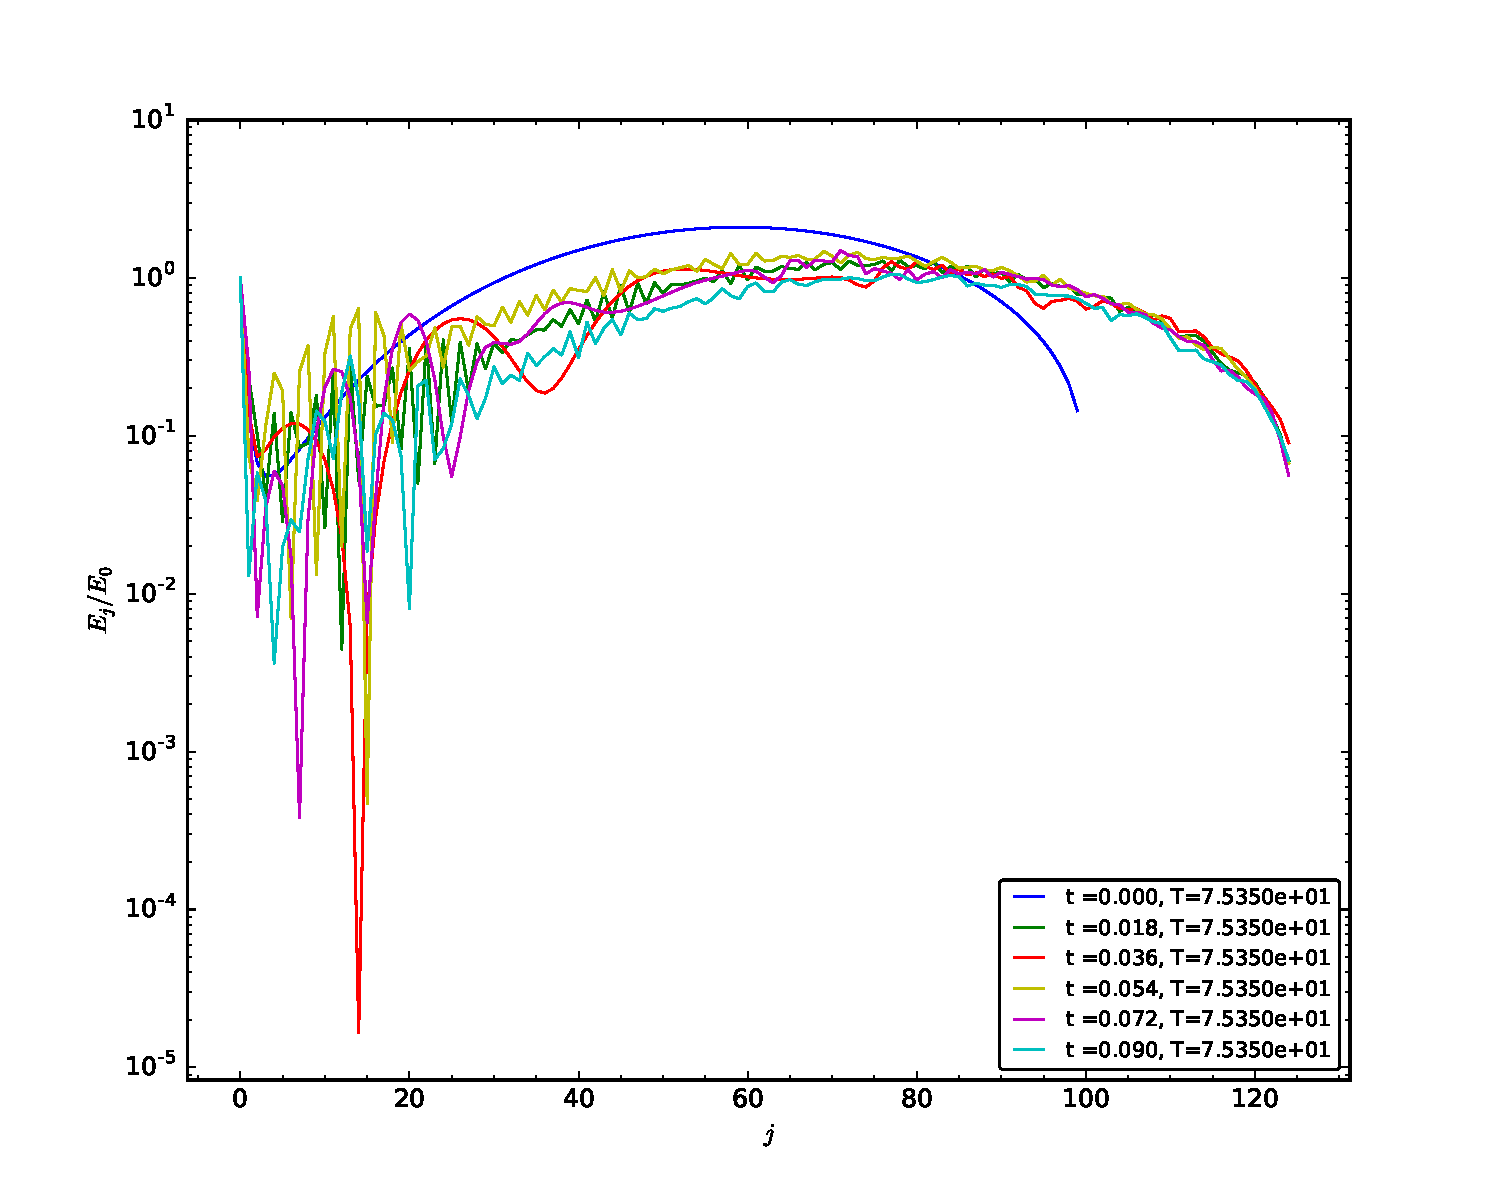
\includegraphics[width=\textwidth]{/Users/bradc/Research/Thesis/PhD/Chapter2/figs/HighTa2_192e-01padj125T6_6711e+01_spectrumevo}
%	\end{subfigure}
%	\;
%	\begin{subfigure}[t]{0.45\textwidth}
%		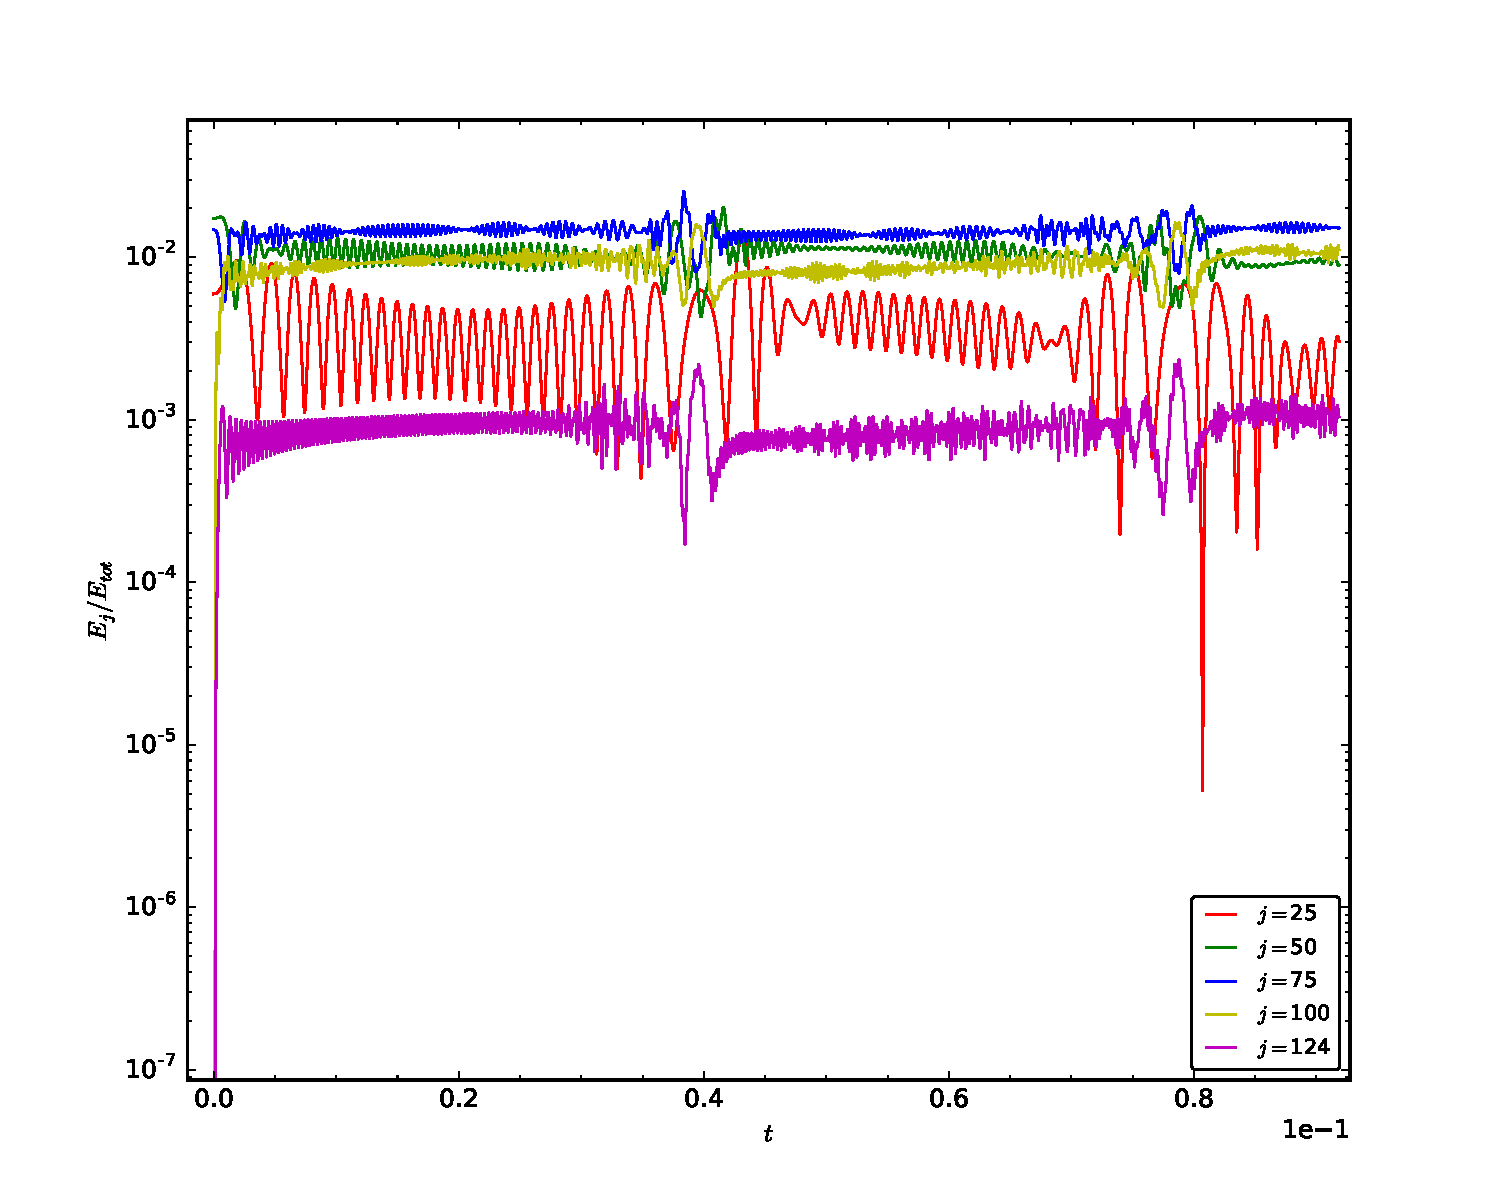
\includegraphics[width=\textwidth]{/Users/bradc/Research/Thesis/PhD/Chapter2/figs/HighTa2_192e-01padj125T6_6711e+01_fullevo}
%	\end{subfigure}
%	\;
%	\begin{subfigure}[t]{0.45\textwidth}
%		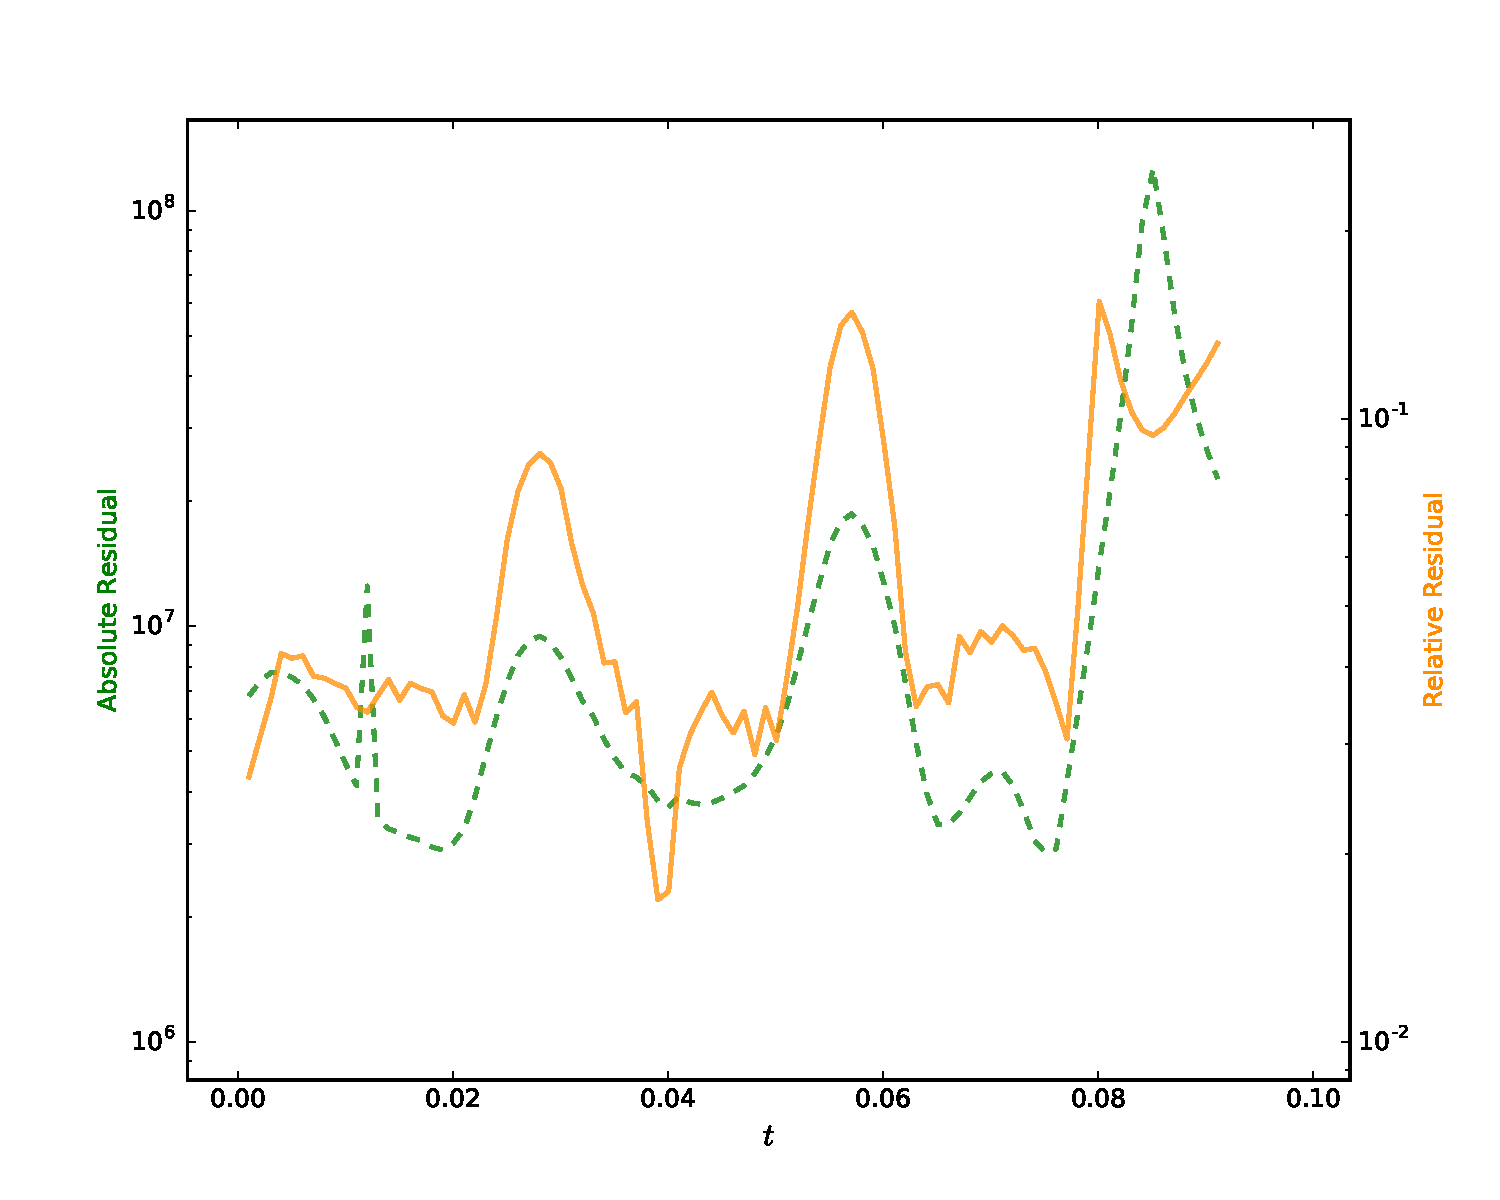
\includegraphics[width=\textwidth]{/Users/bradc/Research/Thesis/PhD/Chapter2/figs/HighTa2_1819e-01padj125T6_6711e+01_Qpresids}
%	\end{subfigure}
%	\;
%	\begin{subfigure}[t]{0.45\textwidth}
%		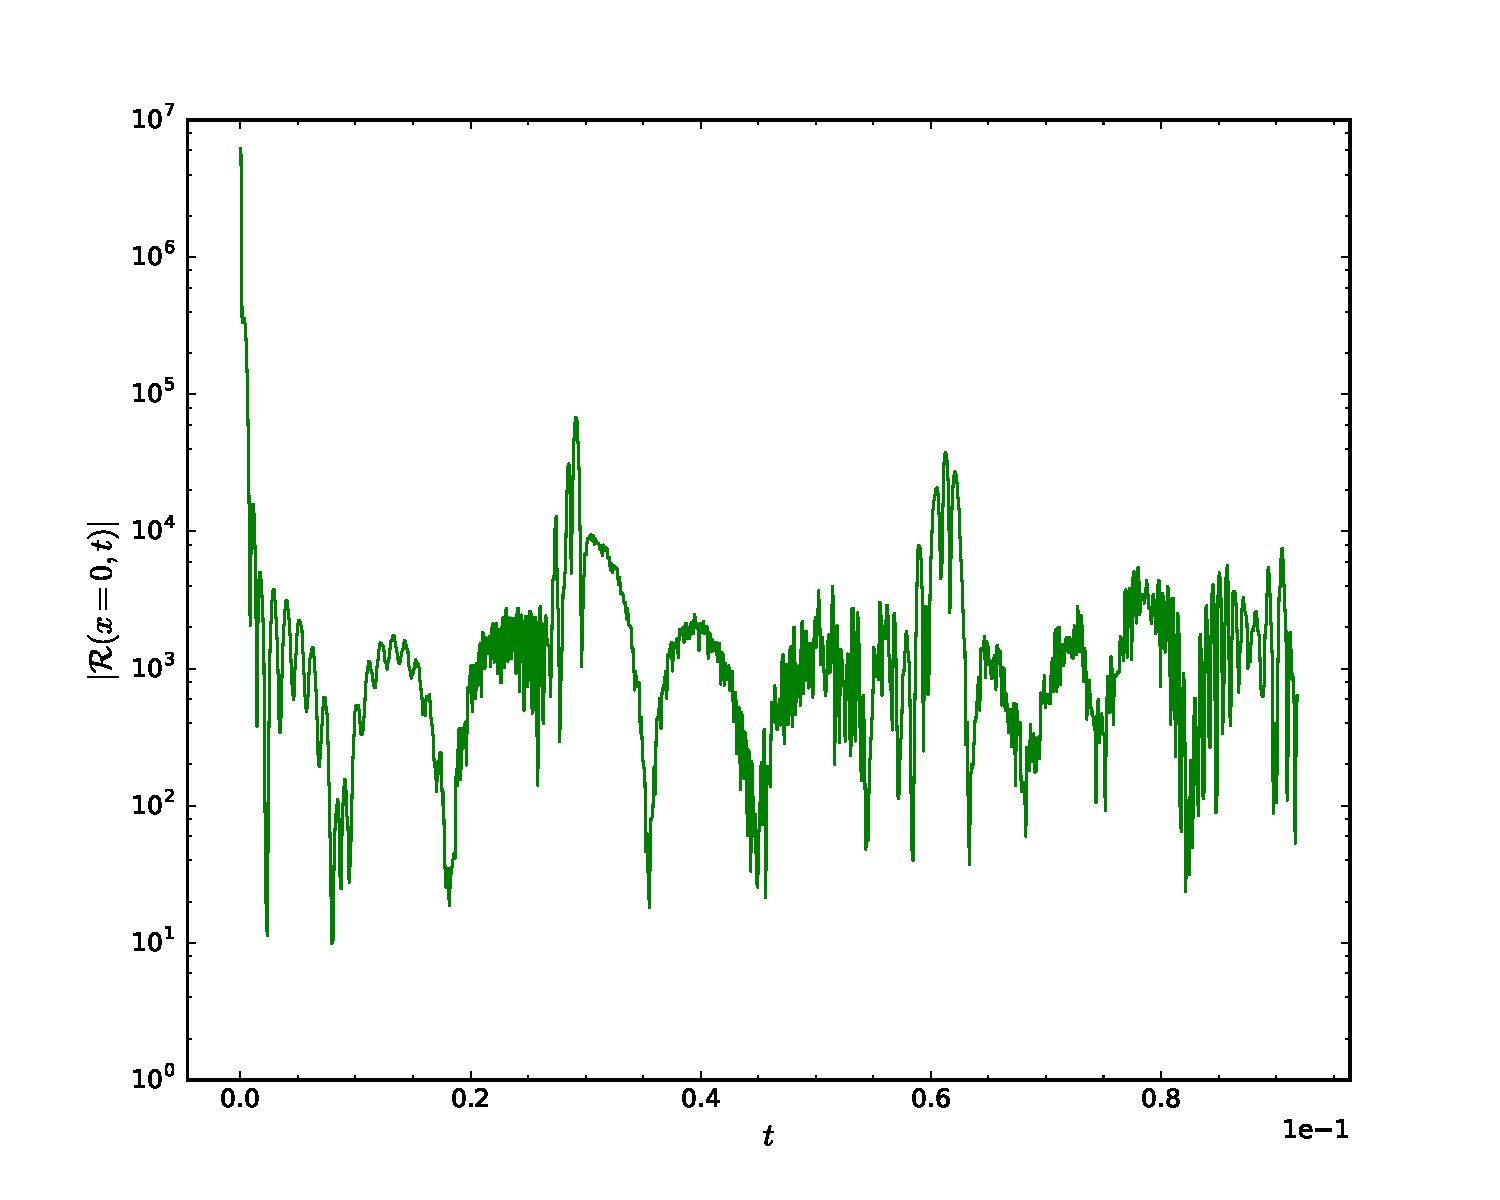
\includegraphics[width=\textwidth]{/Users/bradc/Research/Thesis/PhD/Chapter2/figs/HighTa2_1819e-01padj125T6_6711e+01_ricci}
%	\end{subfigure}
%	\caption[Evolution of the spectrum, absolute and relative residual, and Ricci scalar for a high-temperature solution that has been padded with $25$ extra modes]{Padding the same initial solution from figure~\ref{fig: making highT}, but with only $25$ extra modes.}
%	\label{fig:HighTa2_1819e-01padj125T6_6711e+01_evo}
%\end{figure}

%Finally, consider padding such a solution out to $\jm = 200$. See figure~\ref{fig:HighTa2_1819e-01padj200T6_6711e+01_evo} for results.
%\begin{figure}[h]
%	\centering
%	\begin{subfigure}[t]{0.45\textwidth}
%		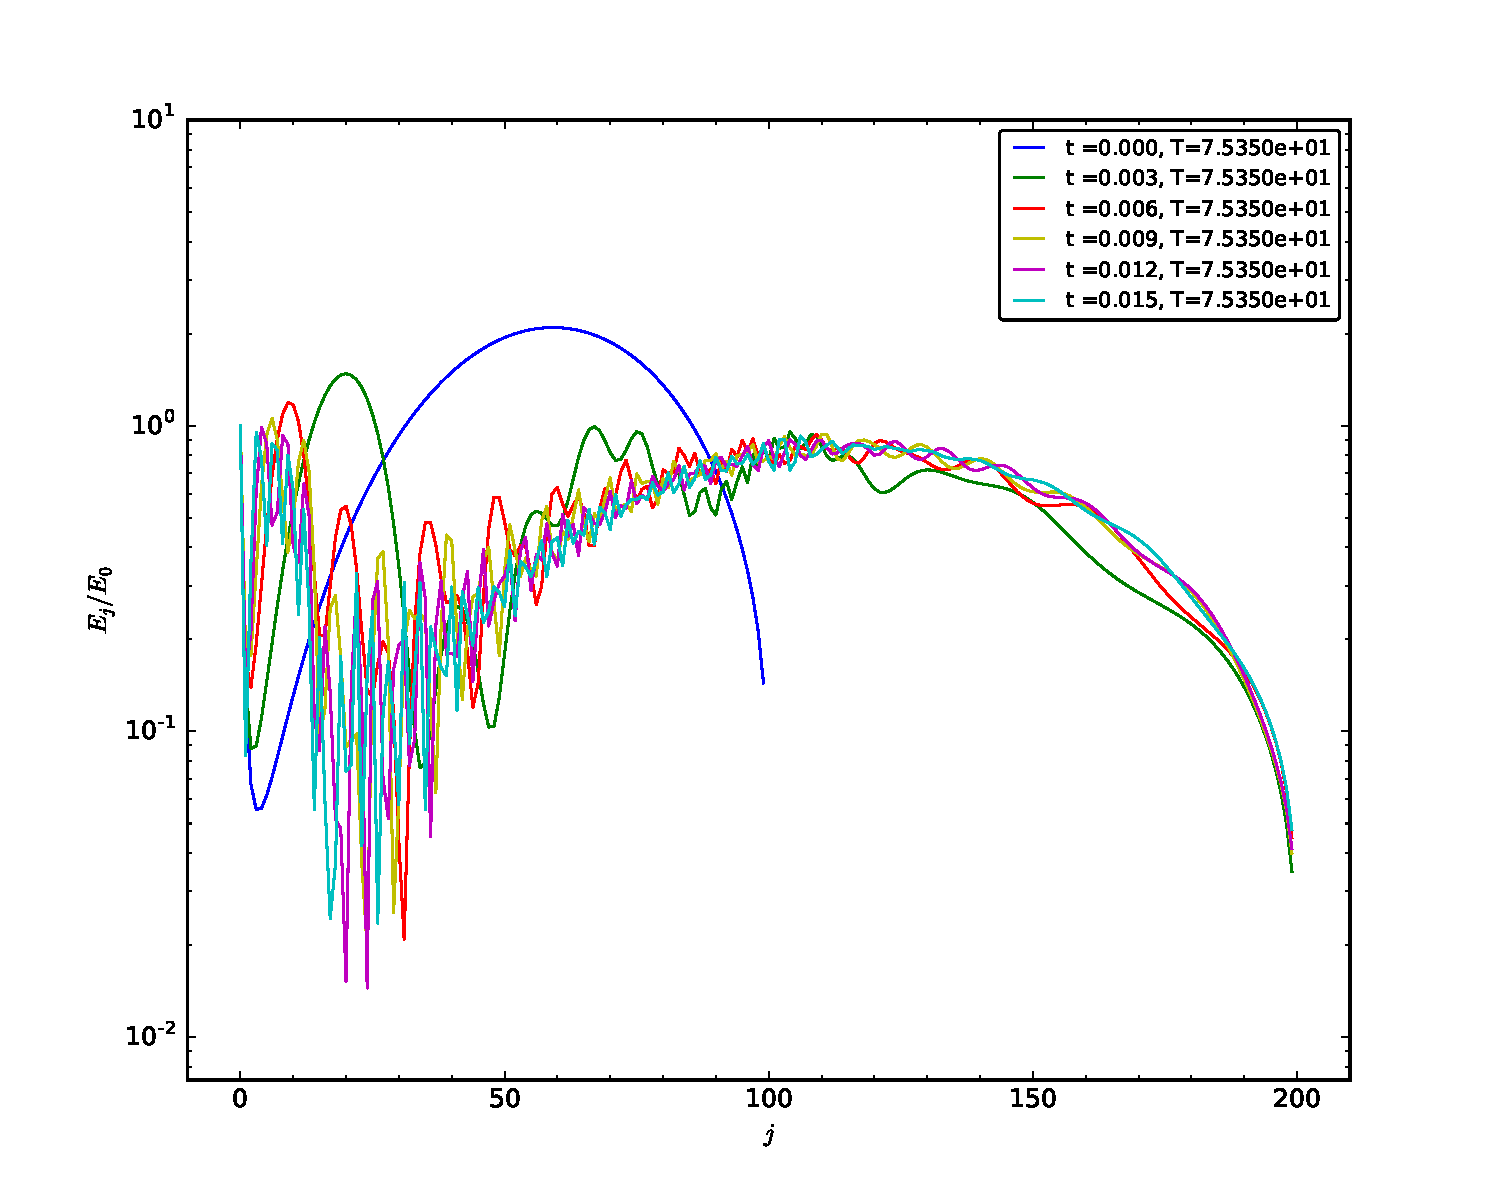
\includegraphics[width=\textwidth]{/Users/bradc/Research/Thesis/PhD/Chapter2/figs/HighTa2_1819e-01padj200T6_6711e+01_specevo}
%	\end{subfigure}
%	\;
%	\begin{subfigure}[t]{0.45\textwidth}
%		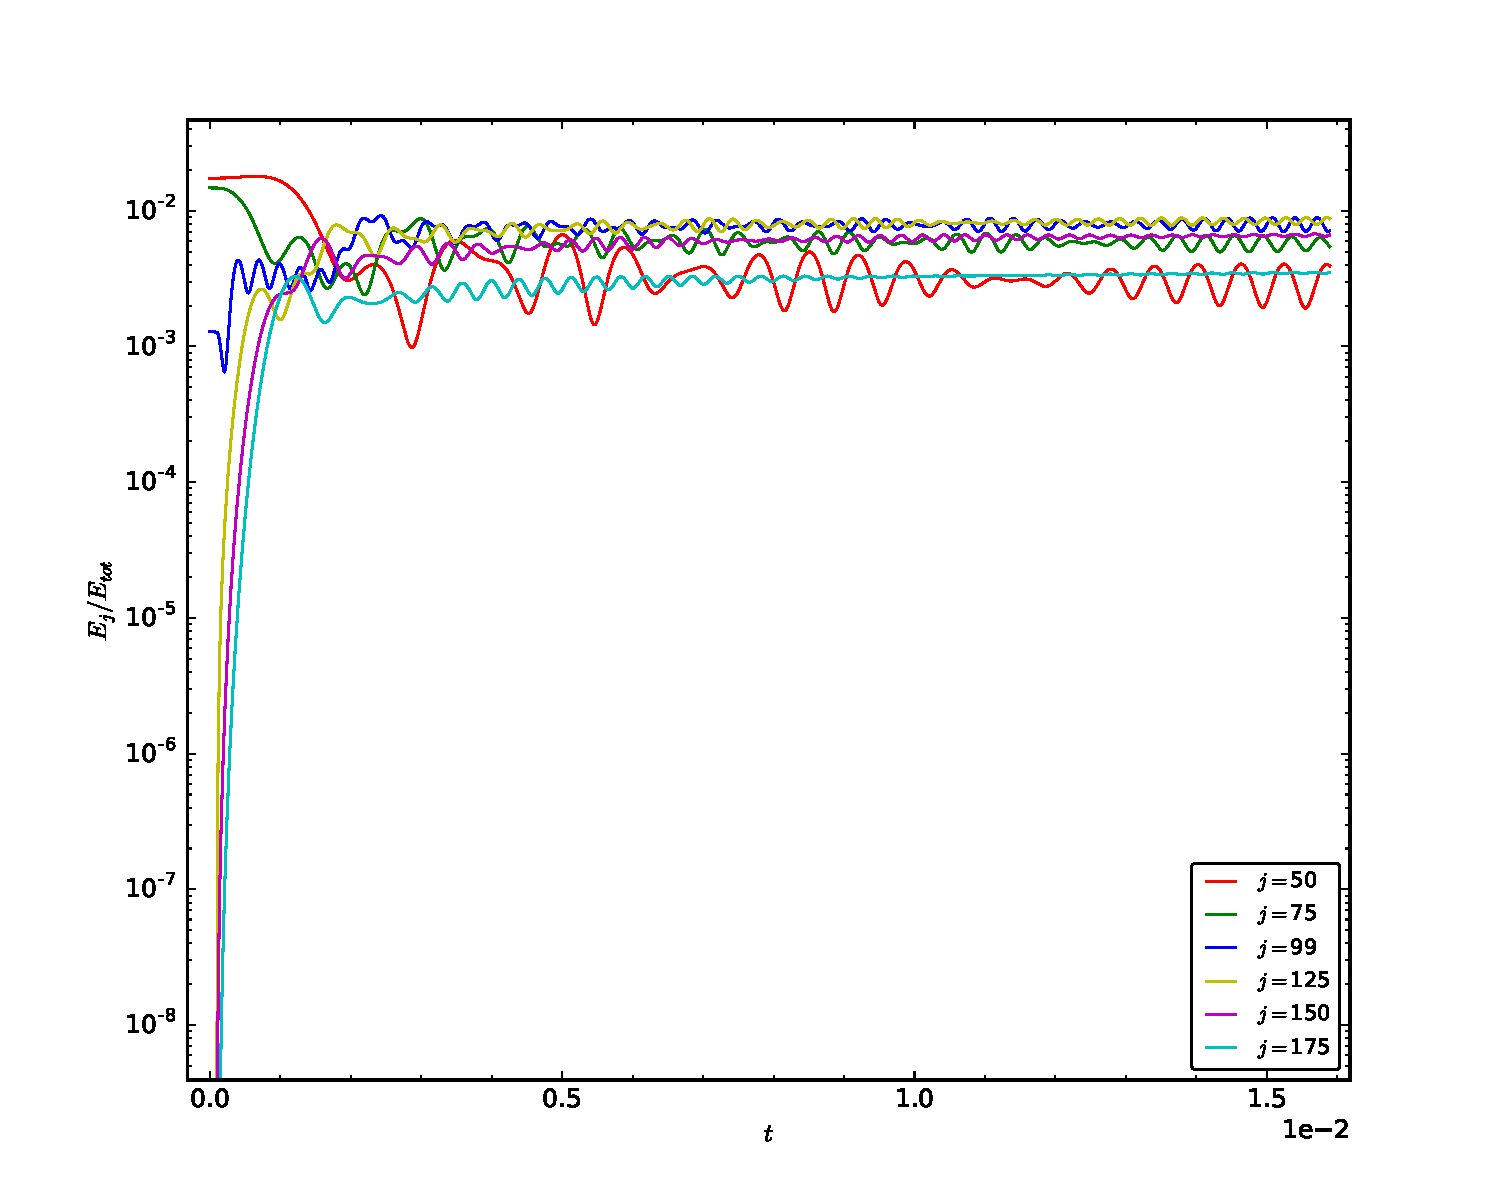
\includegraphics[width=\textwidth]{/Users/bradc/Research/Thesis/PhD/Chapter2/figs/HighTa2_1819e-01padj200T6_6711e+01_modesevo}
%	\end{subfigure}
%	\caption[Evolution of the spectrum of a high-temperature solution padded with $100$ modes]{Padding a $\jm = 100$, high temperature solution to $\jm = 200$ and evolving in time. $\epsilon = 0.1$}
%	\label{fig:HighTa2_1819e-01padj200T6_6711e+01_evo}
%\end{figure}

%The evolved profile of the high-temperature solution can no longer be projected back to the QP solution plane: figure~\ref{fig: HighTa2_1819e-01padj125T6_6711e+01_evolutionprojection}.
%\begin{figure}[h]
%	\centering
%	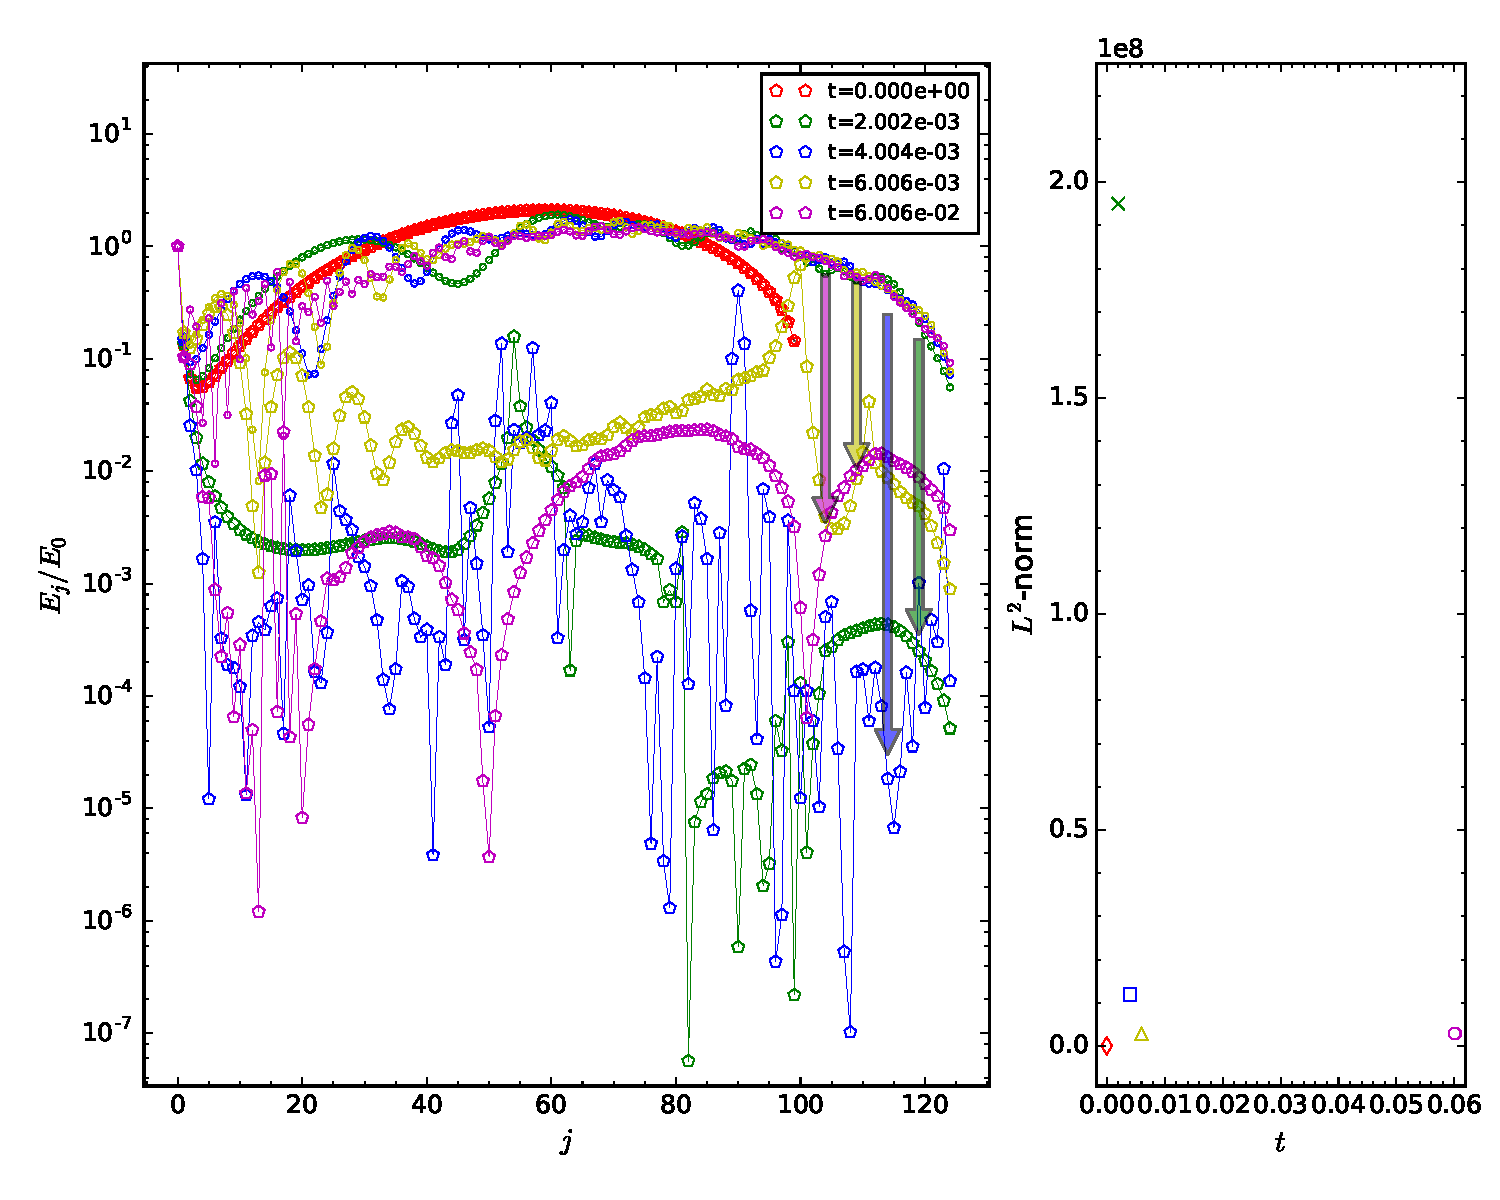
\includegraphics[scale=0.4]{/Users/bradc/Research/Thesis/PhD/Chapter2/figs/HighTa2_1819e-01padj125T6_6711e+01_evolutionprojection}
%	\caption[Evolution of the spectrum of a high-temperature solution padded with $25$ modes]{A high-temperature solution is padded with $25$ extra modes, then evolved in time. Above are the results of projecting back to the QP plane at $t \simeq 0.002, 0.004, 0.006, 0.06$ (red diamond, green cross, blue square, yellow triangle, magenta cirlce).}
%	\label{fig: HighTa2_1819e-01padj125T6_6711e+01_evolutionprojection}
%\end{figure}


%%%%%%%%%%%%%%%%%%%%%%%%%%%%%%%%%%%%%%%%%

\subsection{Perturbing to an Intermediate Temperature Before Reoptimizing}

Here, a QP solution is perturbed to a high temperature without regular projections back to the QP plane. At a pre-determined temperature cutoff, $T = 20.0$, the perturbation procedure is halted and the solution is used as a seed for the nonlinear solver. Instead of projecting to a QP solution at a high temperature, the nonlinear solver converges to a solution with only $T \sim 6.71$. We apply the amplitude-phase evolution procedure to the intermediate $T = 20.0$ solution in order to study how a solution for far away from the QP plane may behave. See figure~\ref{fig:HighTa1_779e-01j100T2_0000e+01evo} for results.

\begin{figure}[h]
	\centering
	\begin{subfigure}[t]{0.45\textwidth}
		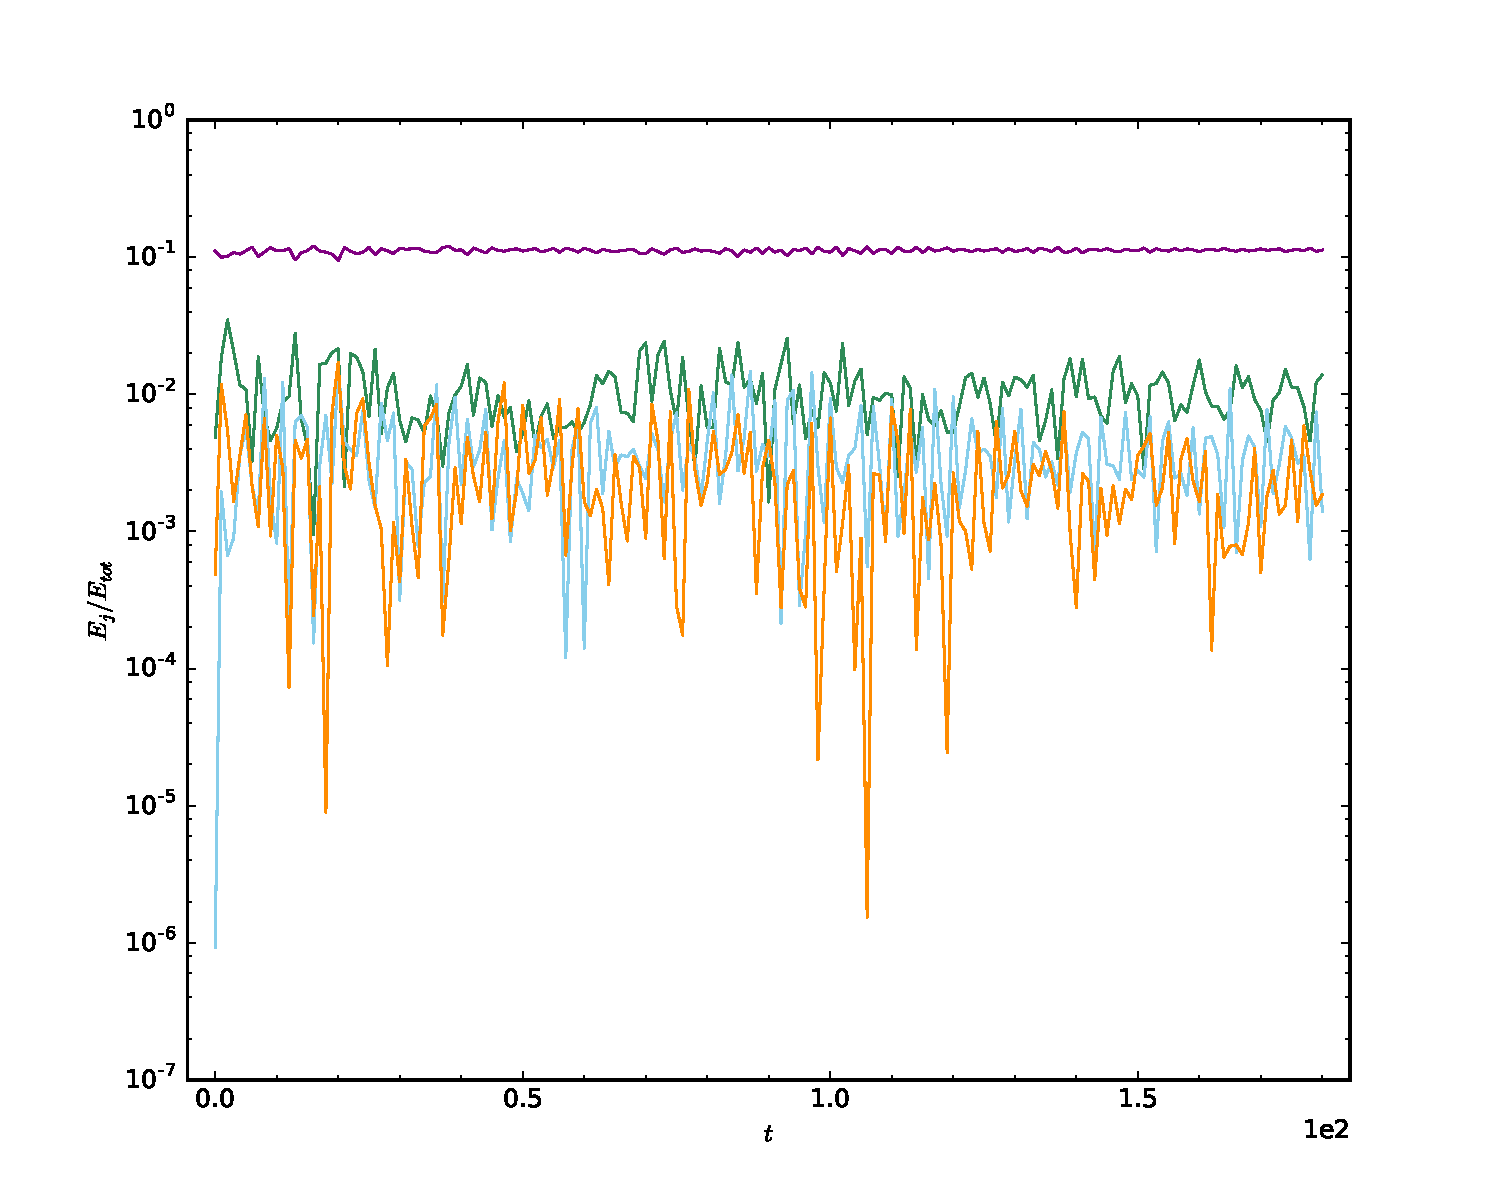
\includegraphics[width=\textwidth]{/Users/bradc/Research/Thesis/PhD/Chapter2/figs/HighTa1_779e-01j100T2_0000e+01_lowjevo}
		\caption{Evolution of the first four modes.}
	\end{subfigure}
	\;
	\begin{subfigure}[t]{0.45\textwidth}
		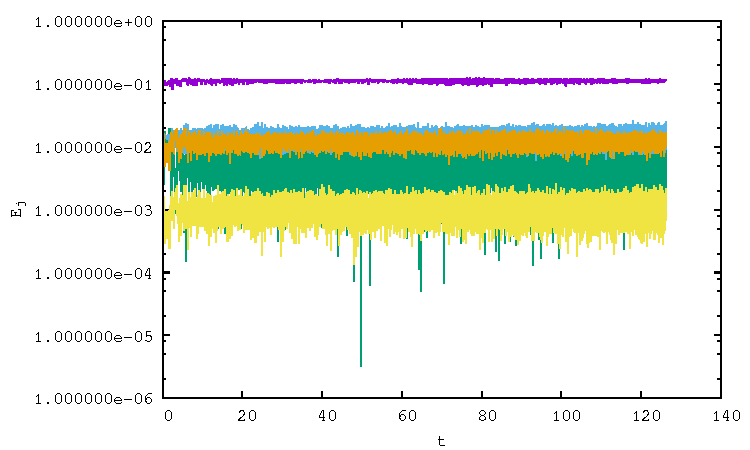
\includegraphics[width=\textwidth]{/Users/bradc/Research/Thesis/PhD/Chapter2/figs/HighTa1_779e-01j100T2_0000e+01_fullevo}
		\caption{Comparative evolution of modes\\ $j=0, 25, 50, 75, 99$.}
	\end{subfigure}
	\;
	\begin{subfigure}[t]{0.45\textwidth}
		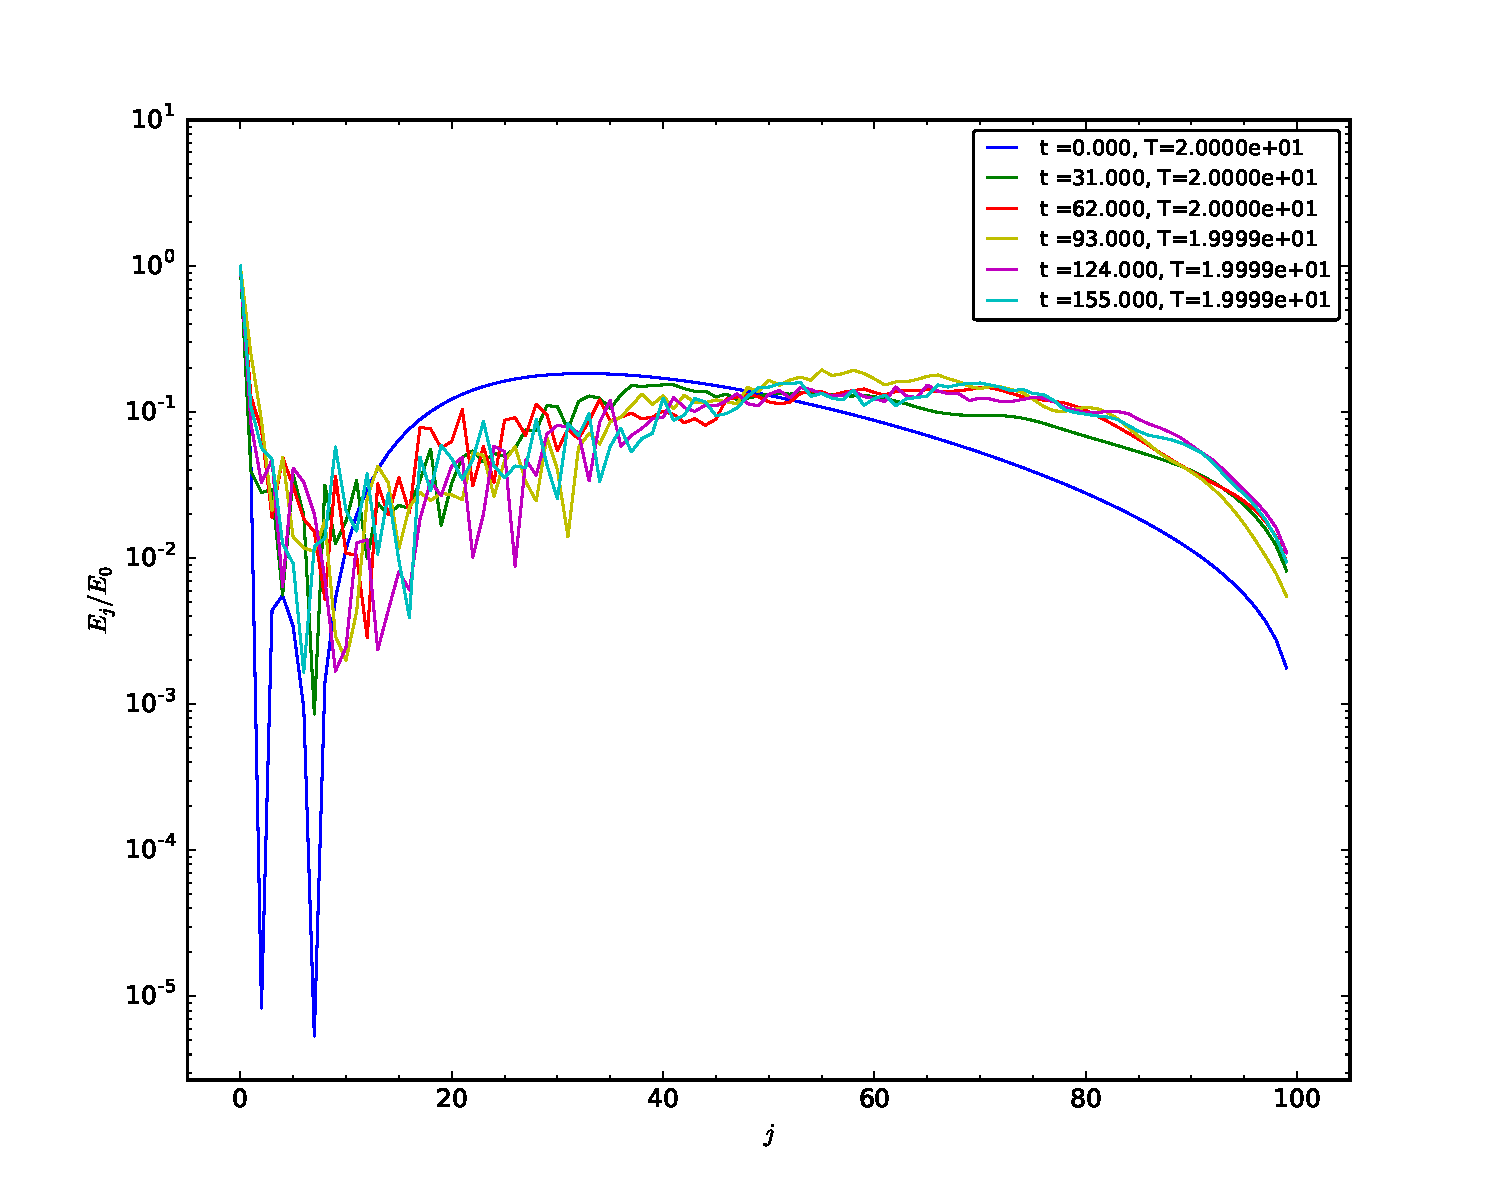
\includegraphics[width=\textwidth]{/Users/bradc/Research/Thesis/PhD/Chapter2/figs/HighTa1_779e-01j100T2_0000e+01_specevo}
		\caption{Energy spectrum at selected times throughout the evolution.}
	\end{subfigure}
	\;
	\begin{subfigure}[t]{0.45\textwidth}
		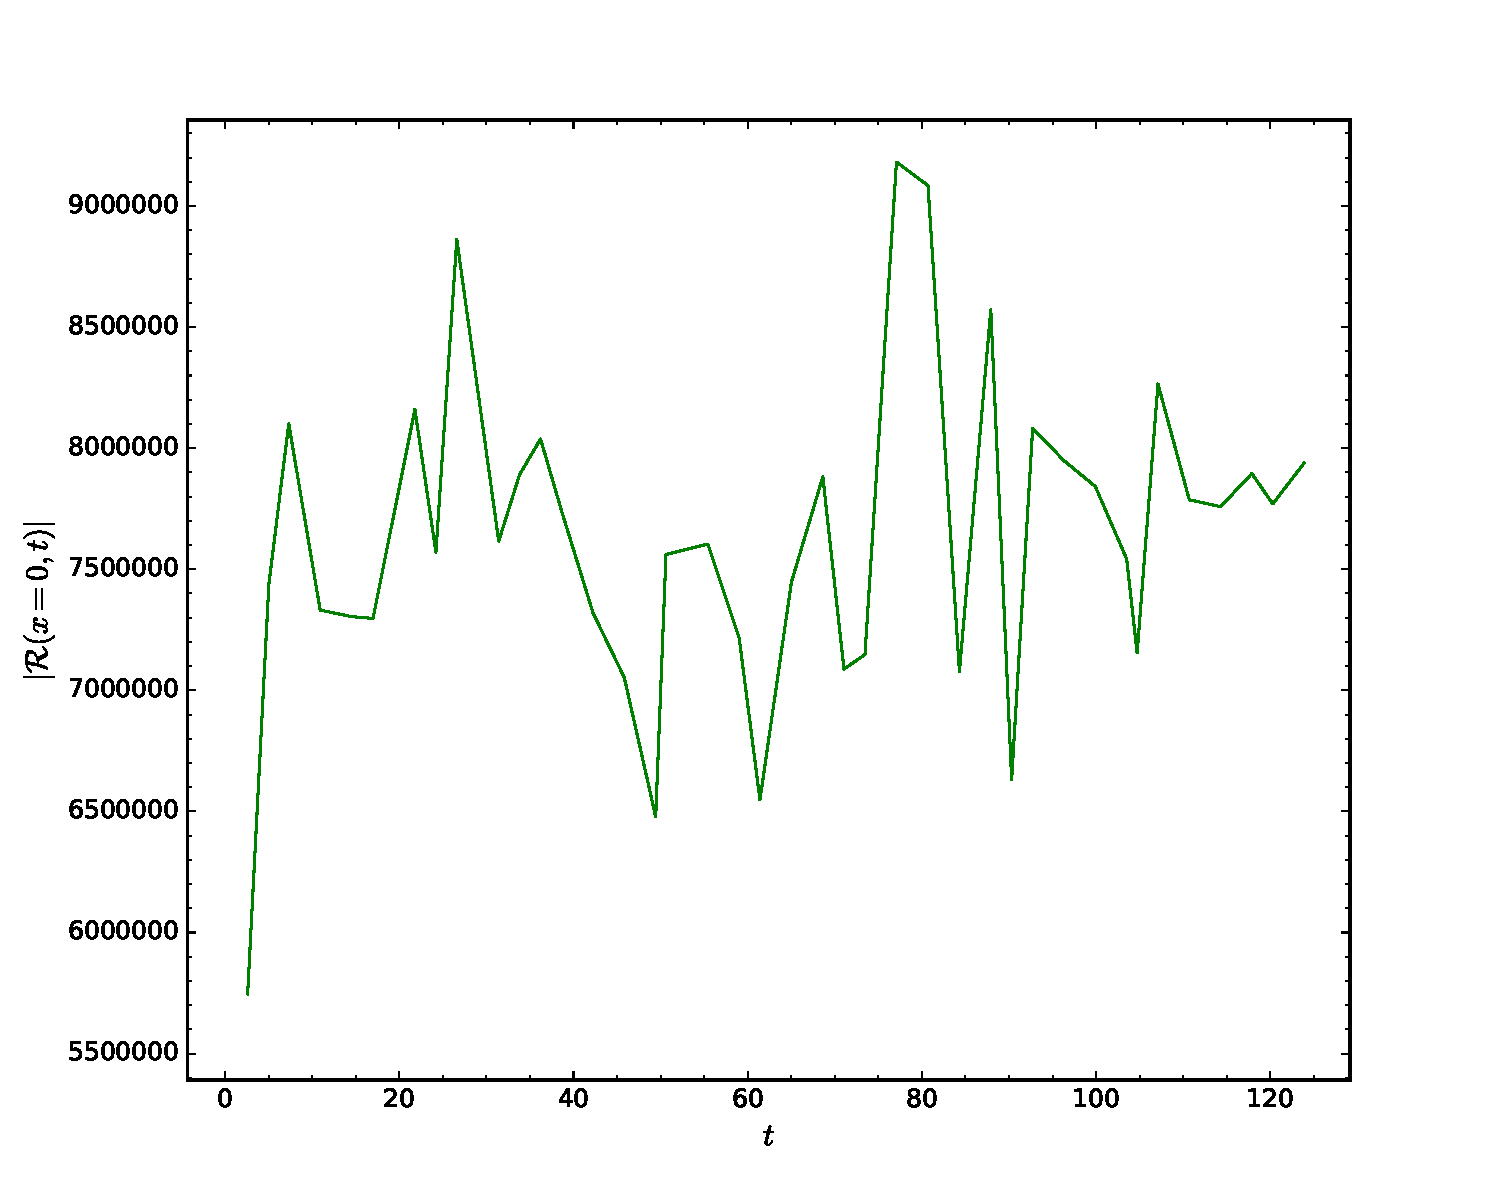
\includegraphics[width=\textwidth]{/Users/bradc/Research/Thesis/PhD/Chapter2/figs/HighTa1_779e-01j100T2_0000e+01_Ricci}
		\caption{The upper envelope of the Ricci scalar at the origin, per light-crossing time.}
	\end{subfigure}
	\caption[Evolution of a high-temperature state that does not satisfy the QP equation]{The evolution of an intermediate, high-temperature solution that \emph{does not} correspond to a solution of the QP equations.}
	\label{fig:HighTa1_779e-01j100T2_0000e+01evo}
\end{figure}

%%%%%%%%%%%%%%%%%%%%%%%%%%%%%%%%%%%%%%%%%

\subsection{Padded Threshold Temperature Solutions}

Padding the threshold temperature solution of $T \sim 5.4$ from $\jm = 100$ to $\jm = 200$ and then evolving in time produces very little change in the spectrum's profile. See figure~\ref{fig:HighTa4_072e-01padj200T5_3921e+00_evo} for results. Despite appearing to remain a high-temperature solution, the evolution of this profile renders it non-QP, as shown in figure~\ref{fig: HighTa4_072e-01padj200T5_3921e+00_projections}. For a more concrete examination, figure~\ref{fig: HighTa4_072e-01spec_vs_pad} shows the threshold temperature solution for $\jm = 200$ as well as padded threshold solutions during their evolution. Under amplitude/phase evolution, the padded solution \emph{does not} approach the known threshold solution.

\begin{figure}[h]
	\centering
	\begin{subfigure}[t]{0.45\textwidth}
		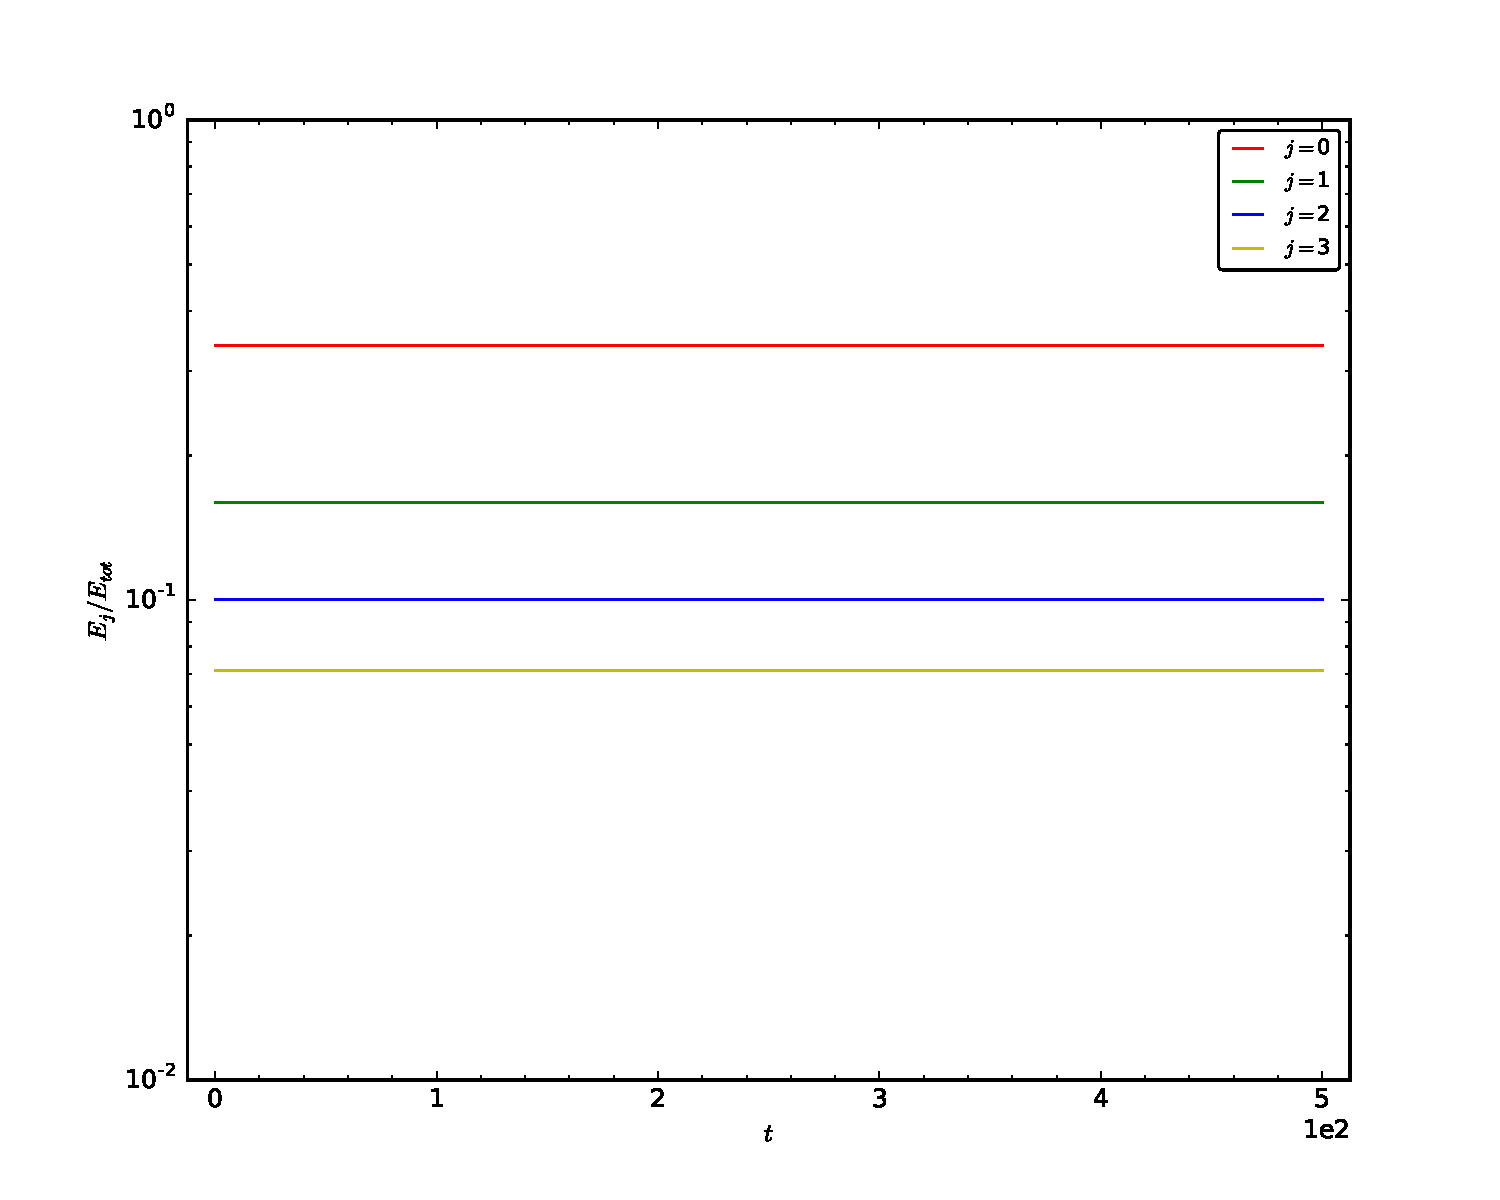
\includegraphics[width=\textwidth]{/Users/bradc/Research/Thesis/PhD/Chapter2/figs/HighTa4_072e-01padj200T5_3921e+00_lowjevo}
	\end{subfigure}
	\;
	\begin{subfigure}[t]{0.45\textwidth}
		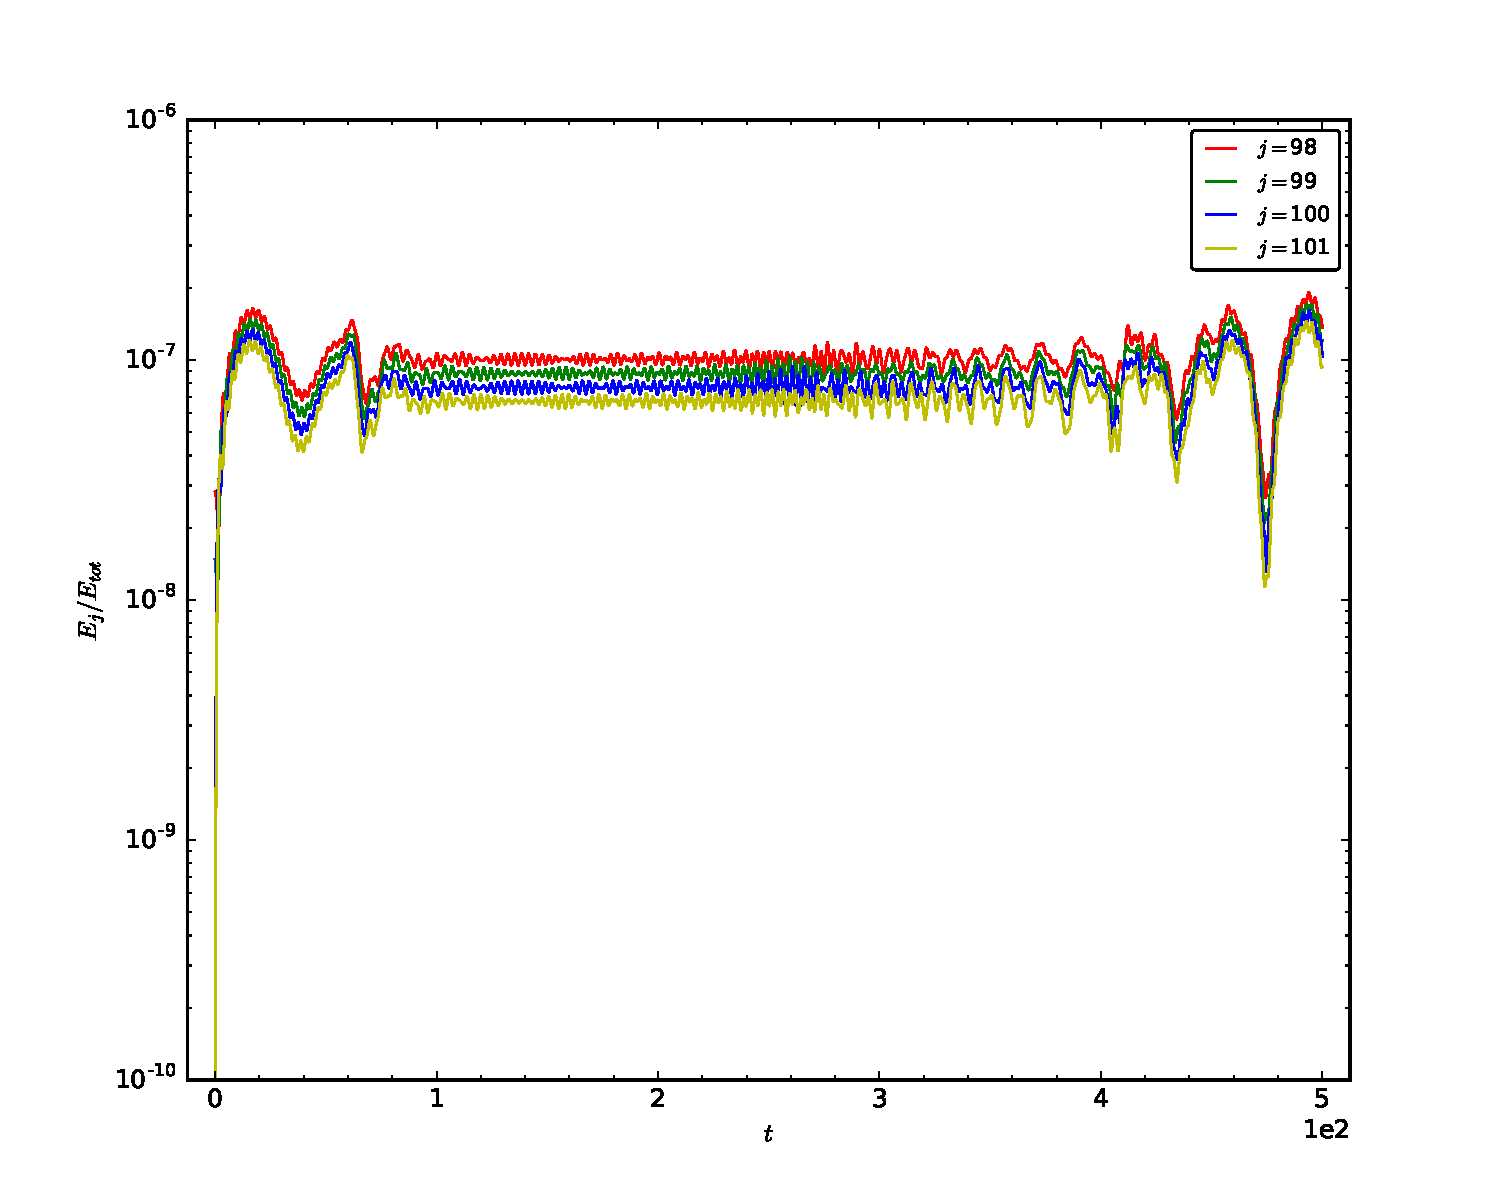
\includegraphics[width=\textwidth]{/Users/bradc/Research/Thesis/PhD/Chapter2/figs/HighTa4_072e-01padj200T5_3921e+00_midjevo}
	\end{subfigure}
	\;
	\begin{subfigure}[t]{0.45\textwidth}
		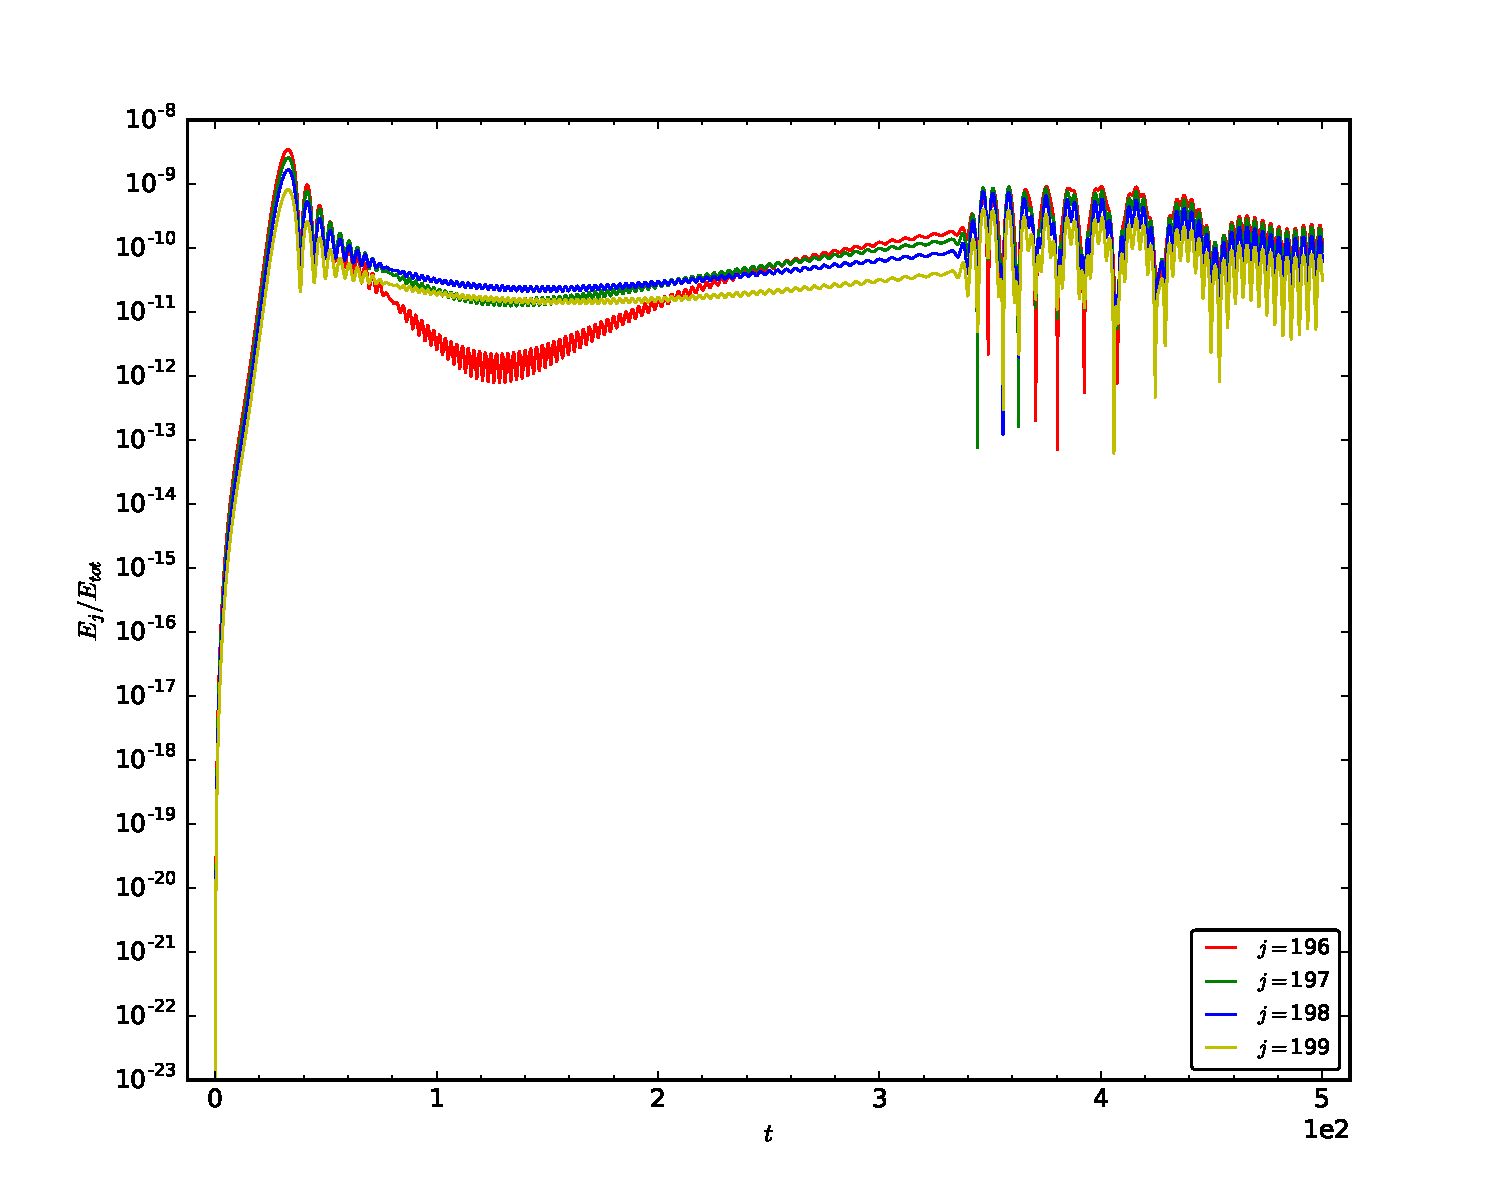
\includegraphics[width=\textwidth]{/Users/bradc/Research/Thesis/PhD/Chapter2/figs/HighTa4_072e-01padj200T5_3921e+00_highjevo}
	\end{subfigure}
	\;
	\begin{subfigure}[t]{0.45\textwidth}
		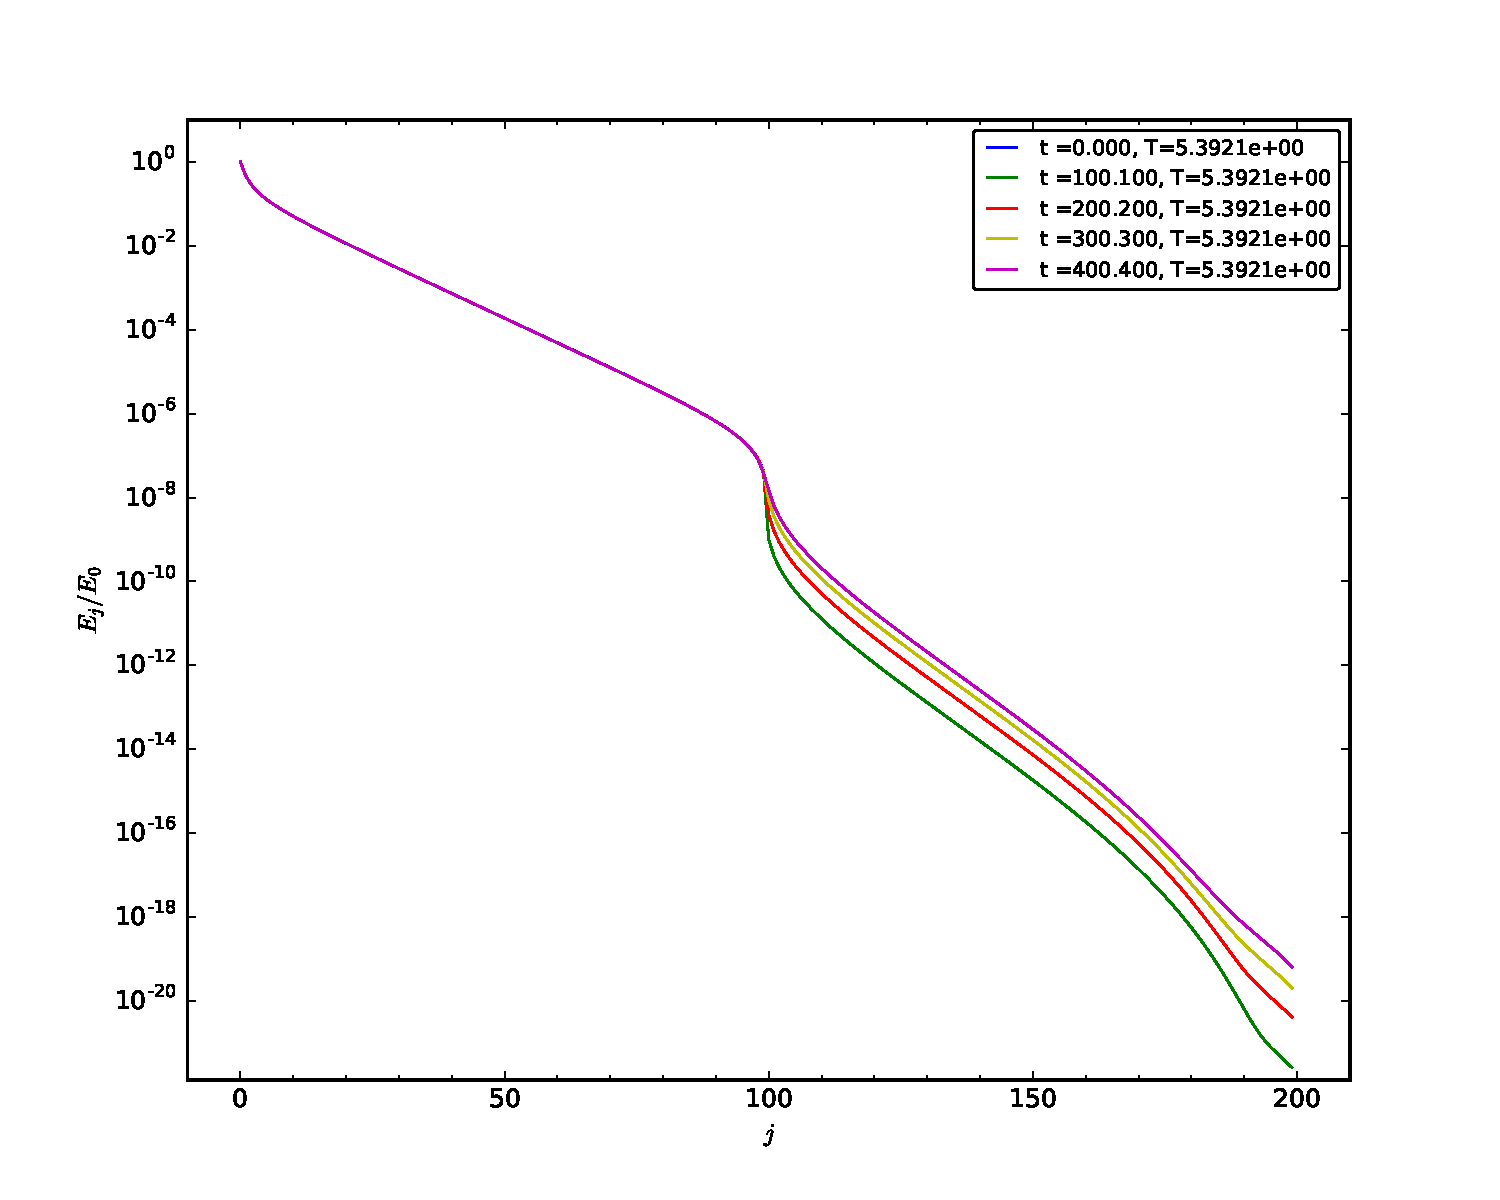
\includegraphics[width=\textwidth]{/Users/bradc/Research/Thesis/PhD/Chapter2/figs/HighTa4_072e-01padj200T5_3921e+00_specevo}
	\end{subfigure}
	\caption[Evolution of the spectrum of a threshold temperature solution that has been padded with $100$ modes]{Padding a threshold temperature solution}
	\label{fig:HighTa4_072e-01padj200T5_3921e+00_evo}
\end{figure}

%\begin{figure}[ht]
%	\centering
%	\begin{subfigure}[t]{0.45\textwidth}
%		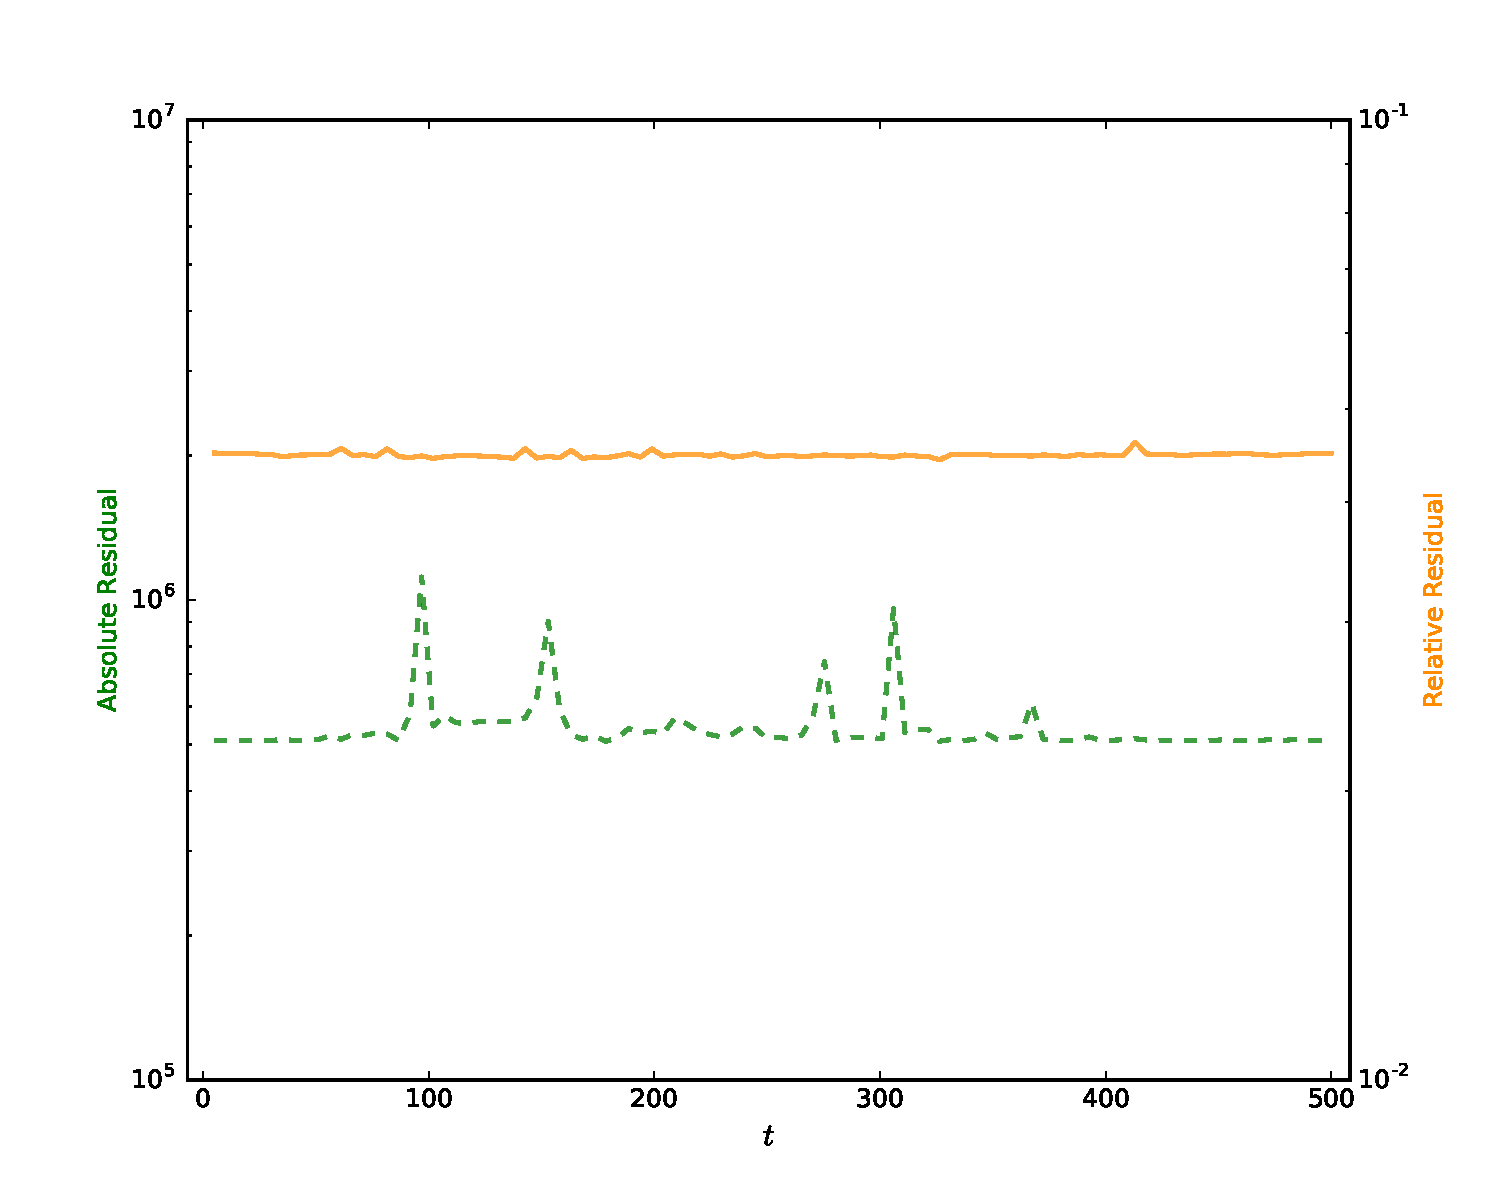
\includegraphics[width=\textwidth]{/Users/bradc/Research/Thesis/PhD/Chapter2/figs/HighTa4_072e-01padj200T5_3921e+00_qpresids}
%		\caption{The residuals of \eqref{qp eqn} during the evolution of the padded threshold temperature solutions shown in figure~\ref{fig:HighTa4_072e-01padj200T5_3921e+00_evo}.}
%	\end{subfigure}
%	\;
%	\begin{subfigure}[t]{0.45\textwidth}
%		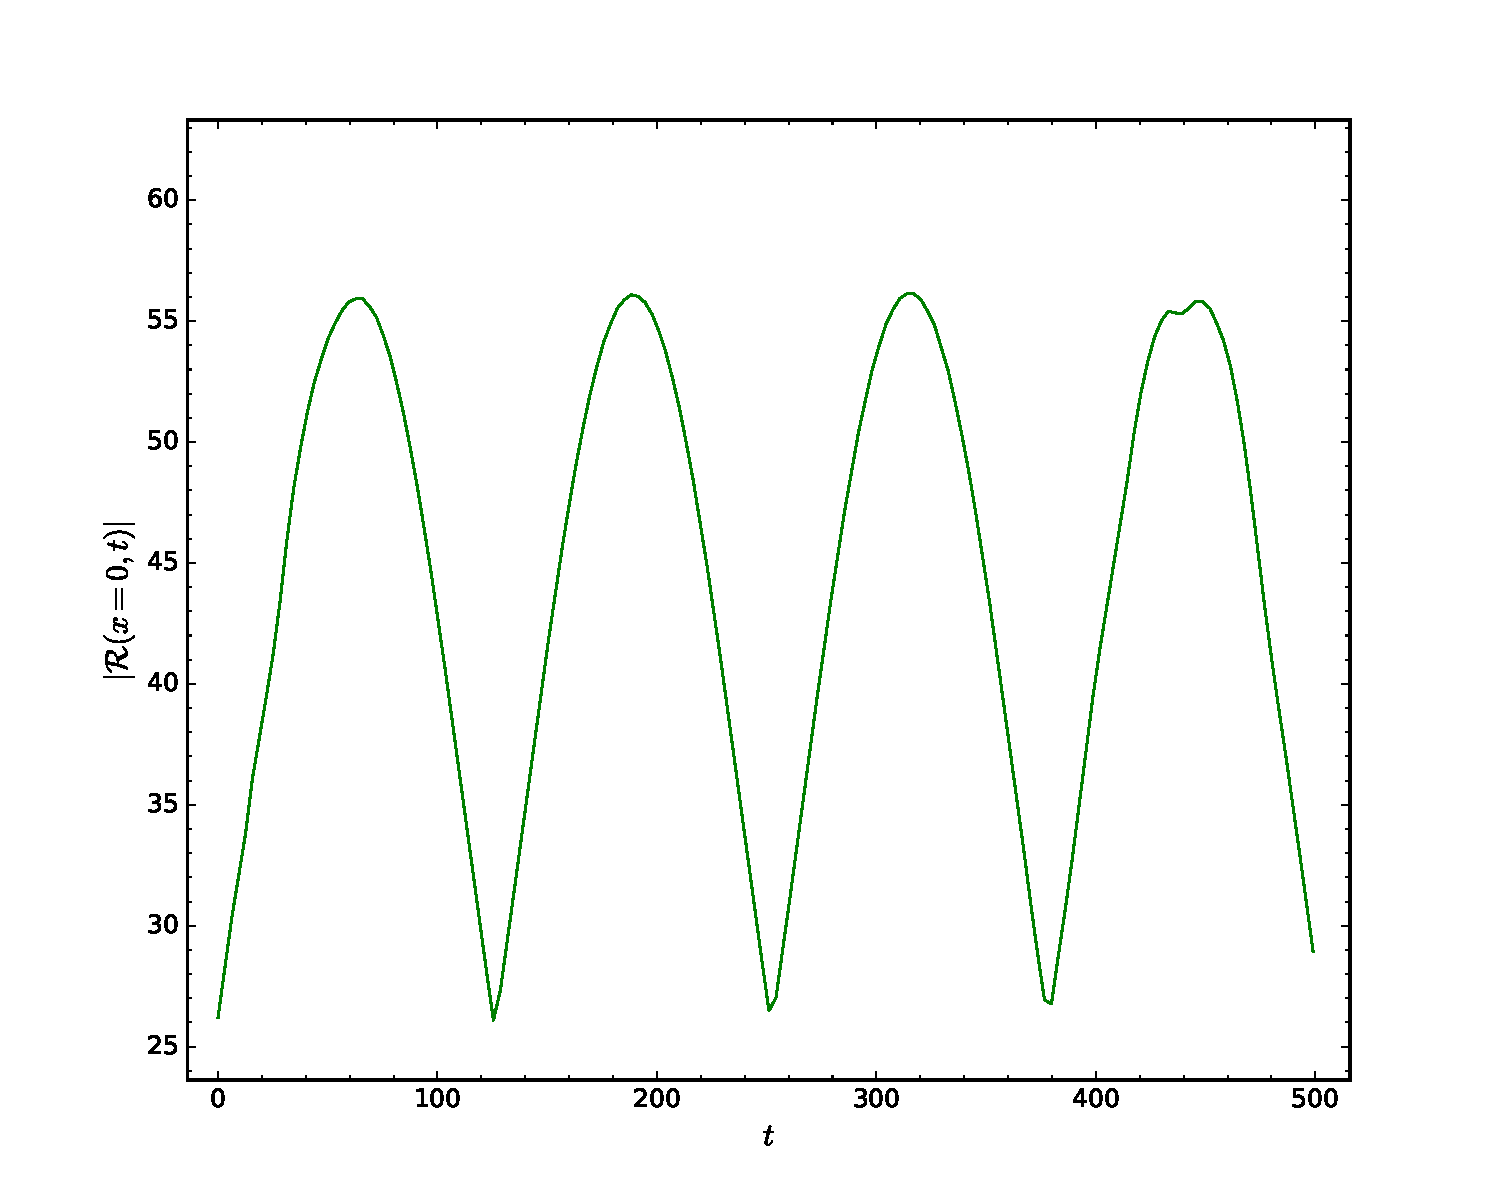
\includegraphics[width=\textwidth]{/Users/bradc/Research/Thesis/PhD/Chapter2/figs/HighTa4_072e-01padj200T5_3921e+00_ricci}
%		\caption{The upper envelope of the Ricci scalar at the origin per light-crossing time for the padded threshold temperature solution.}
%	\end{subfigure}
%	\caption[Padded threshold temperature solutions cannot be projected back to the QP solution plane]{Despite the spectrum of the padded threshold temperature solution (figure~\ref{fig:HighTa4_072e-01padj200T5_3921e+00_evo}) resembling that of lower-temperature QP solutions, these solutions move away from the QP plane and can no longer be projected back.}
%	\label{fig: HighTa4_072e-01padj200T5_3921e+00_projections}
%\end{figure}

\begin{figure}[ht]
	\centering
	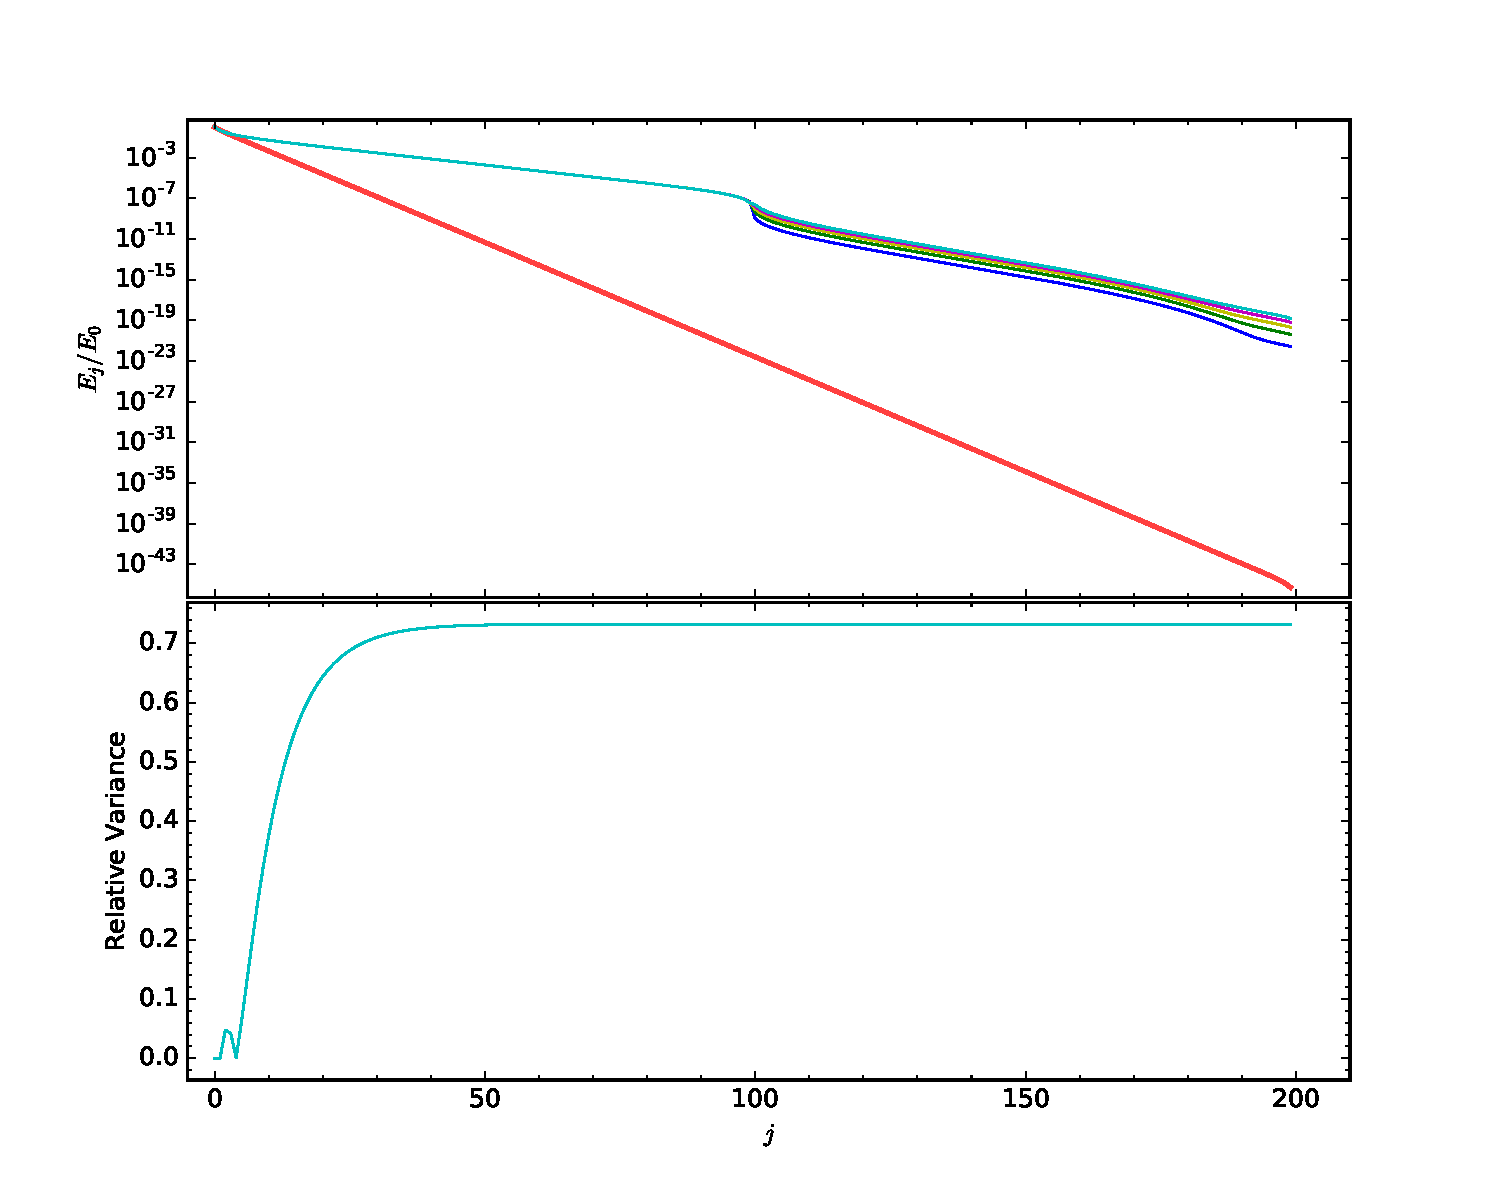
\includegraphics[width=0.75\textwidth]{/Users/bradc/Research/Thesis/PhD/Chapter2/figs/HighTa4_072e-01spec_vs_pad}
	\caption[Comparison between a threshold temperature solution with $j_{max} = 200$ and the evolution of a $j_{max} = 100$ threshold temperature solution that has been padded by $100$ modes]{{\it Top:} Overlay of the known threshold temperature solution for $\jm = 200$ (thick red line) with snapshots of the spectra of a $\jm = 100$ threshold solution that has been padded with zeros to $\jm = 200$ after amplitude/phase evolutions of $\tau =1, 2, 3, 4, 5 \times 10^{-5}$ (blue, green, yellow, magenta, cyan). {\it Bottom:} The absolute value of the difference between the cumulative sums of the $\jm = 200$ threshold temperature solution and each snapshot spectrum (same colouring).}
	\label{fig: HighTa4_072e-01spec_vs_pad}
\end{figure}

%%%%%%%%%%%%%%%%%%%%%%%%%%%%%%%%%%%%%%%%%
%%%%%%%%%%%%%%%%%%%%%%%%%%%%%%%%%%%%%%%%%

\section{Discussion}
\label{sec: discussion}

%%%%%%%%%%%%%%%%%%%%%%%%%%%%%%%%%%%%%%%%%
%%%%%%%%%%%%%%%%%%%%%%%%%%%%%%%%%%%%%%%%%

\paragraph*{Acknowledgments} The work of ND is supported in part by a Natural Sciences and Engineering
Research Council of Canada PGS-D grant to ND, NSF Grant PHY-1606654 at Cornell University, and by a grant from the Sherman Fairchild Foundation. The work of BC and AF is supported by the Natural Sciences and Engineering Research Council of Canada Discovery Grant program. This research was enabled in part by support provided by WestGrid (\href{www.westgrid.ca}{www.westgrid.ca}) and Compute Canada Calcul Canada (\href{www.computecanada.ca}{www.computecanada.ca}).

%%%%%%%%%%%%%%%%%%%%%%%%%%%%%%%%%%%%%%%%%
%%%%%%%%%%%%%%%%%%%%%%%%%%%%%%%%%%%%%%%%%

\begin{subappendices}

%%%%%%%%%%%%%%%%%%%%%%%%%%%%%%%%%%%%%%%%%
%%%%%%%%%%%%%%%%%%%%%%%%%%%%%%%%%%%%%%%%%

\section{Seeding Methods For Non-Linear Solvers}
\label{app: seeding}
While it was originally proposed by \cite{1507.08261} that the appropriate seed value for nonlinear solvers be given by the exponential relation ($j > 1$)
\begin{align}
\label{old seed}
\alpha_j \sim \frac{3 e^{-\mu j}}{2j + 3}
\end{align}
in AdS$_4$, where $\mu = \ln (3 / 5 \alpha_1 )$, as $j_{max}$ increased, the seed values diverged significantly from the true solutions (see figure~\ref{fig: solutionfitting} for a comparison between known QP solutions and the seeds generated by \eqref{old seed}). Although this profile was sufficient for low $j_{max}$ solutions, above $j_{max} \gtrsim 150$, \eqref{old seed} no longer provided an adequate starting guess. To overcome this problem, exponential fitting was applied to the tail values of a known QP solution with lower $j_{max}$. Using this exponential fit, the data was extrapolated to a higher $j_{max}$. 

Care was taken to avoid edge effects due to truncation when choosing the points that constituted the tail of the data. To illustrate the variance of the solution with truncation, we examine a fixed $\alpha_j$ value over a variety of $j_{max}$, starting with $\alpha_j = \alpha_{j_{max}}$. In table~\ref{table: edge effects} we see that the value of $\alpha_{50}$ for QP solutions with $\alpha_1 = 0.2$ becomes impervious to truncation effects once $j_{max} > 55$. 

\begin{table}
		\centering
		\begin{tabular}[t]{| c | c |}
			\hline 
			 $j_{max}$ & $\alpha_{50}$  \\ \hline 
			 $50$ & 1.74597252e-26  \\ \hline
			 $51$ & 1.82668391e-26   \\ \hline
			 $52$ & 1.83346256e-26   \\ \hline
			 $53$ & 1.83408260e-26    \\ \hline
			 $54$ & 1.83414138e-26    \\ \hline
			 $55$ & 1.83414706e-26    \\ \hline
			 $60$ & 1.83414768e-26    \\ \hline
			 $65$ & 1.83414768e-26    \\ \hline
			 $70$ & 1.83414768e-26    \\ \hline
			 $75$ & 1.83414768e-26    \\ \hline
		\end{tabular}
		\caption[Convergence of the real coefficient $\alpha_j$ of the $j = 50$ mode with increasing $j_{max}$]{$\alpha_{50}$ values for various $j_{max}$ QP solutions.}
		\label{table: edge effects}
\end{table}

\begin{figure}[h]
\centering
	\begin{subfigure}[t]{0.45\textwidth}
		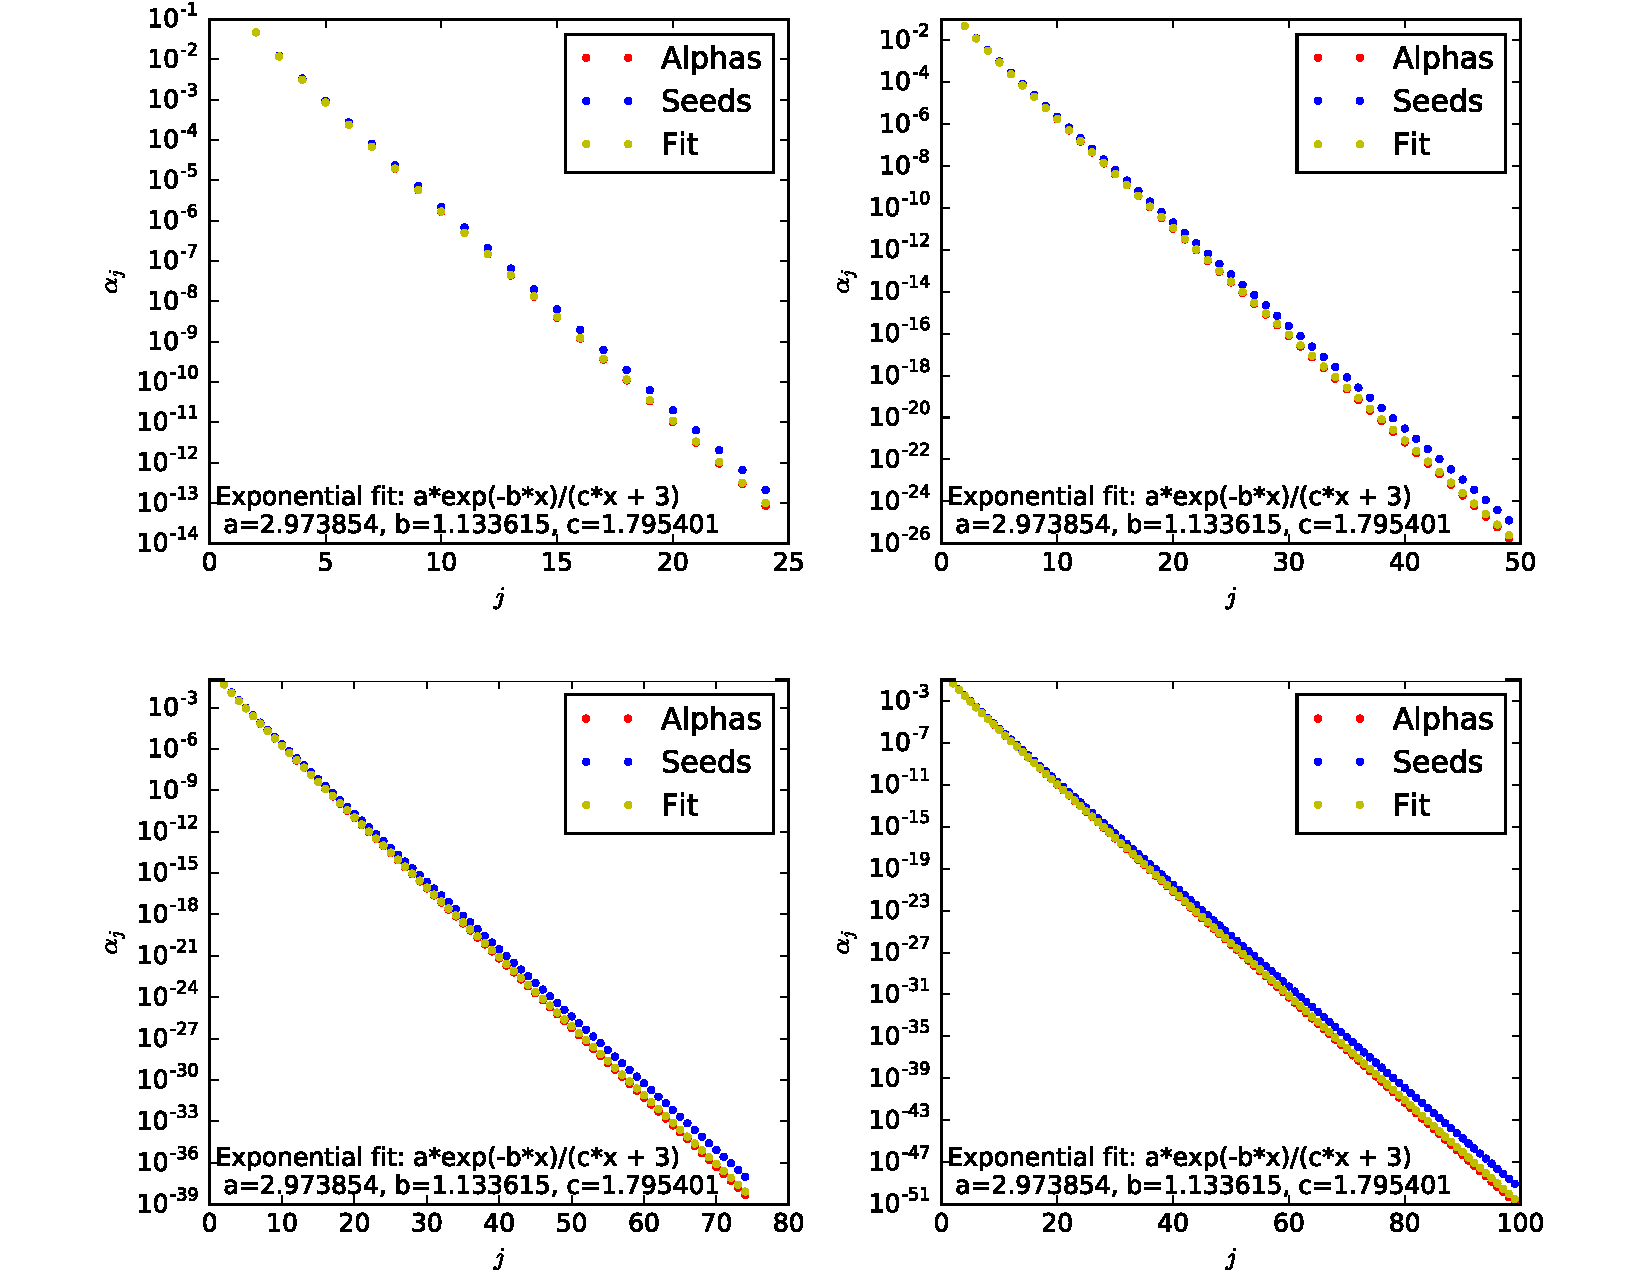
\includegraphics[width=\textwidth]{/Users/bradc/Research/Thesis/PhD/Chapter2/figs/SolutionsvsFits_a2_00e-01_pg1}
		\caption{$\alpha_1 = 0.2$ QP solutions for $j_{max} \in [25,100]$.}
		\label{fig: sol vs fit low jmax}
	\end{subfigure}
	\quad
	\begin{subfigure}[t]{0.45\textwidth}
		\includegraphics[width=\textwidth]{/Users/bradc/Research/Thesis/PhD/Chapter2/figs/SolutionsvsFits_a2_00e-01_pg2}
		\caption{$\alpha_1 = 0.2$ QP solutions for $j_{max}~\in~[140,200]$.}
		\label{fig: sol vs fit high jmax}
	\end{subfigure}
	\caption[Comparison of seed values to known QP solutions and exponential fitting]{A comparison of seeds predicted by \eqref{old seed} to known QP solution. Also included for comparison are the results of fitting the QP solutions to a generic exponential fit.}
	\label{fig: solutionfitting}
\end{figure}
			

To err on the side of caution, the modes $[ j_{max} - 30,\: j_{max} - 10]$ were used from each QP solution to provide more accurate seed values for $j_{max} + 25$ solutions. See figure~\ref{fig: tail fitting} for a comparison of seed values generated by tail fitting to actual QP solutions. The solutions found using this method of seeding versus those found from the seeding given in \eqref{old seed} had relative differences on the order of $10^{-14}$ (see figure~\ref{fig: seedvsunseed}).

\begin{figure}[h]
	\centering
	\begin{subfigure}[t]{0.45\textwidth}
  		\includegraphics[width=\textwidth]{/Users/bradc/Research/Thesis/PhD/Chapter2/figs/TailFitPlot}
  		\caption{Fitting the tail of the $j_{max} = 175$ spectrum to construct a seed for $j_{max} = 200$ at fixed $\alpha_1 = 0.2$. Also included is actual QP spectrum for $j_{max} = 200$.}
  		\label{fig: tail fitting}
	\end{subfigure}
	\;
	\begin{subfigure}[t]{0.45\textwidth}
		\includegraphics[width=0.97\textwidth]{/Users/bradc/Research/Thesis/PhD/Chapter2/figs/SeedvsUnseed}
		\caption{Relative difference between $\alpha_1=0.2$ QP solutions found using tail-fitting and those from the exponential profile~\eqref{old seed}.}
		\label{fig: seedvsunseed}
	\end{subfigure}
	\caption[Illustrating the tail fitting procedure]{The process and result of tail fitting the $\alpha_j$ spectra of QP solutions to generate better seed values.}
   	\label{fig: fit & resids}
\end{figure}

%%%%%%%%%%%%%%%%%%%%%%%%%%%%%%%%%%%%%%%%%
%%%%%%%%%%%%%%%%%%%%%%%%%%%%%%%%%%%%%%%%%

\section{Auxiliary Integrals For Calculating the $T, R, S$ Coefficients}
\label{app: integrals}

The auxiliary coefficients $X, Y, W, W^*, A$, and $V$ allow the symmetries of the $T, R$ and $S$ coefficients to be more easily recognized and therefore reduce the number of total calculations involved in determining \eqref{T calc} - \eqref{S calc}. These auxiliary coefficients are written simply in terms of the eigenfunctions in \eqref{ttf eigens} and their derivatives. Explicitly, they are
\begin{align}
\label{X int}
X_{ijk\ell} &= \int^{\pi/2}_0 dx \, e'_i(x) e_j(x) e_k(x) e_\ell(x) \sin(x) \cos(x) \left( \tan(x) \right)^{d-1} \\
\label{Y int}
Y_{ijk\ell} &= \int^{\pi/2}_0 dx \, e'_i(x) e_j(x) e'_k(x) e'_\ell(x) \sin(x) \cos(x) \left( \tan(x) \right)^{d-1} \\
\label{W int}
W_{ijk\ell} &= \int^{\pi/2}_0 dx \, e_i(x) e_j(x) \sin(x) \cos(x) \int^x_0 dy \, e_k(y) e_\ell(y) \left( \tan(y) \right)^{d-1} \\
\label{W* int}
W^*_{ijk\ell} &= \int^{\pi/2}_0 dx \, e'_i(x) e'_j(x) \sin(x) \cos(x) \int^x_0 dy \, e_k(y) e_\ell(y) \left( \tan(y) \right)^{d-1} \\
\label{A int}
A_{ij} &= \int^{\pi/2}_0 dx \, e'_i(x) e'_j(x) \sin(x) \cos(x) \\
\label{V int}
V_{ij} &= \int^{\pi/2}_0 dx \, e_i(x) e_j(x) \sin(x) \cos(x) \, .
\end{align}

In terms of these coefficients, the TTF source terms are given by
\begin{align}
\label{T calc}
T_\ell &= \frac{1}{2} \ol^2 X_{\ell\ell\ell\ell} + \frac{3}{2} Y_{\ell\ell\ell\ell} + 2\omega_\ell^4 W_{\ell\ell\ell\ell} + 2\omega_\ell^2 W^*_{\ell\ell\ell\ell} - \omega_\ell^2 (A_{\ell\ell} + \omega_\ell^2 V_{\ell\ell} ) \\
\label{R calc}
R_{i\ell} &=\frac{1}{2} \left(\frac{\oi^2 + \ol^2}{\ol^2 - \oi^2}\right) (\omega_\ell^2 X_{i\ell\ell i} - \omega_i^2 X_{\ell ii\ell}) + 2\left(\frac{\ol^2 Y_{i\ell i\ell } - \oi^2 Y_{\ell i\ell i}}{\ol^2 - \oi^2} \right) \nonumber \\
&+ \left(\frac{\oi^2 \ol^2}{\ol^2 - \oi^2}\right) (X_{i\ell \ell i} - X_{\ell i\ell i}) + \frac{1}{2} (Y_{ii\ell \ell } + Y_{\ell \ell ii}) + \oi^2 \ol^2 (W_{\ell \ell ii} + W_{ii\ell \ell }) \nonumber \\
&+ \oi^2 W^*_{\ell \ell ii} + \ol^2 W^*_{ii\ell \ell } - \ol^2 (A_{ii} + \omega_i^2 V_{ii} ) \\
\label{S calc}
S_{ijk\ell } &= -\frac{1}{4} \left( \frac{1}{\omega_i + \omega_j} + \frac{1}{\omega_i - \omega_k} + \frac{1}{\omega_j - \omega_k} \right) (\omega_i \omega_j \omega_k X_{\ell ijk} - \omega_\ell  Y_{i\ell jk}) \nonumber \\
& - \frac{1}{4} \left( \frac{1}{\omega_i + \omega_j} +\frac{1}{\omega_i - \omega_k} - \frac{1}{\omega_j - \omega_k} \right) (\oj \ok \ol X_{ijk\ell } - \oi Y_{jik\ell } ) \nonumber \\
& -\frac{1}{4} \left( \frac{1}{\oi + \oj} - \frac{1}{\oi - \ok} + \frac{1}{\oj -\ok} \right) (\oi \ok \ol X_{jik\ell } - \oj Y_{ijk\ell } ) \nonumber \\
& -\frac{1}{4} \left( \frac{1}{\oi + \oj} - \frac{1}{\oi - \ok} - \frac{1}{\oj - \ok} \right) (\oi \oj \ol X_{kij\ell } - \ok Y_{ikj\ell }) \, .
\end{align}



%%%%%%%%%%%%%%%%%%%%%%%%%%%%%%%%%%%%%%%%%
%%%%%%%%%%%%%%%%%%%%%%%%%%%%%%%%%%%%%%%%%

\section{Frequency of Solution Checking}
\label{app: reop freq}

The frequency of applying the nonlinear solver to project back down to the QP solution plane is an important part of ensuring that the perturbative method remains applicable. If QP solutions are perturbed by too large an energy, or for too many iterations, the intermediate solutions may not be close enough to the solution plane to provide an adequate seed value. Such was the concern when examining the purported high-temperature solutions from existing sources.

For example, consider the process of applying perturbations of $\delta E = 0.01\%$ up to some intermediate temperature without projecting back to the QP plane, then projecting back every 100 iterations until a maximum temperature is reached. Starting with the QP solution corresponding to $\alpha_1 = 0.2$, the lower panel of figure~\ref{fig: reop check} shows the result of repeated perturbations of $\delta E = 0.01\%$ that are not projected back the to QP plane.

\begin{figure}[h]
	\centering
	\begin{subfigure}[t]{0.48\textwidth}
		\includegraphics[width=\textwidth]{/Users/bradc/Research/Thesis/PhD/Chapter2/figs/j50T17cont_4paper}
		\label{fig: reop check j50}
	\end{subfigure}
	\;
	\begin{subfigure}[t]{0.48\textwidth}
		\includegraphics[width=\textwidth]{/Users/bradc/Research/Thesis/PhD/Chapter2/figs/j150T17cont_4paper}
		\label{fig: reop check j150}
	\end{subfigure}
\caption[Comparison of spectra and temperatures for different projection frequencies between $j_{max}=50$ and $j_{max} = 150$ solutions]{{\it Left}: the result of unchecked perturbations of a $j_{max} = 50$ QP solution up to an intermediate temperature before switching to regular checking. {\it Right}: the same procedure is applied to a $j_{max}=150$ QP solution.}
\label{fig: reop check}
\end{figure}

The behaviour of the spectra differ for the low and high $j_{max}$ cases. For the $j_{max}=50$ solutions, the spectra in the lower panel of the figure can be remain smooth through more than 27,000 iterations of $\delta E$ perturbations. When a temperature of approximately 17 is reached, the spectrum is used as a seed value for the nonlinear solver and a smooth solution is found. Continuing with the same $\delta E$, but reapplying the nonlinear solver produces mixed results; the temperatures of increasing iterations do not increase monotonically, but do always project back to a solution with nearly the same temperature. However, the spectra themselves develop kinks by iteration 3,100 that are indicative of a change of sign in the alpha values and a breakdown of the perturbative condition. Because only a small number of modes are considered, numerical solutions are still found by the Newton-Raphson solver but no longer represent physical states. Continuing this procedure, we find that the solver fails to find a solution even at the modest temperature of $T \simeq 38$.

The behaviour of the $j_{max}=150$ solutions is consistent with their lower-mode number counterparts, albeit more pronounced. We see that kinks in the spectrum develop even when the nonlinear solver has not been applied. The intermediate solution used as a seed for the nonlinear solver did not project back to a nearby temperature, instead falling from $T \simeq 14.2$ to $T \simeq 4.3$. As the perturbative procedure continued, projection back to the QP plane was only possible in for a short time before no solution could be found. Note the numerous spikes in the energy spectrum shown in the upper panel. For $j_{max} = 150$, we conclude that no physically relevant high-temperature solutions exist, even as low as $T \simeq 4.76$.

\end{subappendices}

%%%%%%%%%%%%%%%%%%%%%%%%%%%%%%%%%%%%%%%%%
%%%%%%%%%%%%%%%%%%%%%%%%%%%%%%%%%%%%%%%%%

\end{document}

%%%%%%%%%%%%%%%%%%%%%%%%%%%%%%%%%%%%%%%%%
%%%%%%%%%%%%%%%%%%%%%%%%%%%%%%%%%%%%%%%%%
